%%%%% Basic setup for one-sided printing:
%%%%% Margins: left 40mm, right 25mm, top and bottom 25mm (but beware, LaTeX adds 1in by itself)
%%%%% ---------------------------------------------------------------
\documentclass[12pt, a4paper]{report}
\usepackage{geometry}
\setlength\textwidth{145mm}
\setlength\textheight{247mm}
\setlength\oddsidemargin{15mm}
\setlength\evensidemargin{15mm}
\setlength\topmargin{0mm}
\setlength\headsep{0mm}
\setlength\headheight{0mm}
\newcommand{\openright}{\clearpage}

%%%%% Base setup for two-sided printing:
%%%%% ---------------------------------------------------------------
% \documentclass[12pt, a4paper, twoside, openright]{report}
% \setlength\textwidth{145mm}
% \setlength\textheight{247mm}
% \setlength\oddsidemargin{15mm}
% \setlength\evensidemargin{0mm}
% \setlength\topmargin{0mm}
% \setlength\headsep{0mm}
% \setlength\headheight{0mm}
% \let\openright=\cleardoublepage

%%%%% Czech language settings
%%%%% ---------------------------------------------------------------
% \usepackage[czech]{babel}
% \ifx\uv\undefined\newcommand{\uv}[1]{,,#1``}\fi
\usepackage [english]{babel}
\usepackage [autostyle, english = american]{csquotes}
\MakeOuterQuote{"}

%%%%% Preamble with settings and macros
%%%%% ---------------------------------------------------------------
%%%%% Setting the input encoding of the files: UTF-8
%%%%% ---------------------------------------------------------------
\usepackage[utf8]{inputenc}

%%%%% Setting the language of the document
%%%%% ---------------------------------------------------------------
\usepackage{setspace}
\onehalfspacing
\usepackage{indentfirst}
\setlength{\parindent}{0pt}
\setlength{\parskip}{0.75\baselineskip}

%%%%% Color definitions
%%%%% ---------------------------------------------------------------
\usepackage{xcolor}
\definecolor{unicorn_blue}{HTML}{0B2A70}
\definecolor{unicorn_blue_light}{HTML}{40C8D3}
\definecolor{chart1}{HTML}{2D7DD2}  % Clear Blue
\definecolor{chart2}{HTML}{6C969D}  % Golden Yellow
\definecolor{chart3}{HTML}{97CC04}  % Lime Green
\definecolor{chart4}{HTML}{EEB902}  % Orange
\definecolor{chart5}{HTML}{474647}  % Dark Gray
\definecolor{chart6}{HTML}{F45D01}  % Steel Blue
\definecolor{chart7}{HTML}{9B6B6C}  % Dusty Rose
\definecolor{chart8}{HTML}{556F44}  % Forest Green

%%%%% Setting the color boxes/frames
%%%%% ---------------------------------------------------------------
\usepackage{tcolorbox}
% gray box preset
\newtcolorbox{gray-box}[1]{colback=gray!5!white,colframe=gray!50!black,title=#1}
\newtcolorbox{blue-box}[1]{colback=unicorn_blue!5!white,colframe=unicorn_blue,title=#1}


%%%%% Setting the colors and syntax of the code
%%%%% ---------------------------------------------------------------
% TODO: Define the colors
\usepackage{fvextra}
\usepackage{colortbl} % for colored rows/columns
\definecolor{codekeyword}{rgb}{0.0,0.3,0.7}
\definecolor{codestring}{rgb}{0.4,0.4,0.8}
\definecolor{codecomment}{rgb}{0.2,0.2,0.2}
\definecolor{codejsdoc}{rgb}{0.4,0.4,0.4}
\definecolor{codelinenum}{rgb}{0.8,0.8,0.8}
\definecolor{lightyellow}{rgb}{255, 255, 224}

% minted package setup
\usepackage[outputdir=dist]{minted}
\setminted{
	frame=none,
	breaklines=true,
	fontsize=\footnotesize,
	tabsize=2,
	linenos,
	numbersep=5pt,
	xleftmargin=0pt,
	baselinestretch=1.2,
	style=friendly,
%   TODO: highlighting not working
	highlightcolor=\color{lightyellow},
	keywordstyle=\color{codekeyword},
	stringstyle=\color{codestring},
	commentstyle=\color{codecomment}\itshape,
	morecomment=[s][\color{codejsdoc}]{/**}{*/},
	numberstyle=\footnotesize\color{codelinenum}
}

% listings package setup
\usepackage{listings}
\lstset{
	basicstyle=\ttfamily,
	columns=fullflexible,
	frame=single,
	breaklines=true,
	showstringspaces=false,
	keywordstyle=\bfseries,
	commentstyle=\itshape\color{gray},
	captionpos=t
}

% wrap long URLs
\PassOptionsToPackage{hyphens}{url}

%%%%% Tables
%%%%% ---------------------------------------------------------------
\usepackage{tabularx}

%%%%% Additional useful packages
%%%%% ----------------------------------------------------------------
\usepackage{amsmath}
\usepackage{amsfonts}
\usepackage{amsthm}
\usepackage{bm}
\usepackage{graphicx}
\usepackage[labelfont=bf]{caption}
\newcommand{\sourceDefaultLabel}{Own creation}
\newcommand{\sourceLabel}{Source:}
\newcommand{\source}[1][\sourceDefaultLabel]{\caption*{\hfill\footnotesize{\sourceLabel~\textit{#1}}}}
\usepackage{psfrag}
\usepackage{fancyvrb}
\usepackage[numbers]{natbib}
\usepackage{usebib}
\usepackage{tikz}
\usepackage{bbding}
\usepackage{icomma}
\usepackage{dcolumn}
\usepackage{booktabs}
\usepackage{paralist}
\usepackage{float}
\usepackage{subcaption}
\usepackage{epigraph}
\newcommand\foreign[1]{\emph{#1}}
\usepackage{pdfpages}
\usepackage{nameref}
% will create a reference to a chapter, section, ... including the number and in bold
\renewcommand{\fullref}[1]{\textbf{\nameref{#1}}}

% utils
\newcommand{\todo}[1]{\newline\textcolor{red}{\textbf{TODO:} #1}\newline}
\newcommand{\note}[1]{\newline\textcolor{blue}{\textbf{NOTE:} #1}\newline}
\newcommand{\theEvent}{\textbf{The Event}}
\newcommand{\theOrganizer}{\textbf{The Organizer}}
\newcommand{\eg}{e.g.,}

% Formatting numbers
\usepackage{siunitx} % for number formatting
% configure siunitx for Czech number formatting
\sisetup{
	group-separator={,},
	group-minimum-digits=4,
	round-mode=places,
	round-precision=0,
	output-decimal-marker={.},
}
\newcommand{\fmtnum}[1]{\num{#1}}
\newcommand{\fmtnump}[2][2]{\num[round-mode=places, round-precision=#1]{#2}}
\newcommand{\fmtczk}[1]{\num{#1}~CZK}
\newcommand{\fmtczkp}[2][2]{\num[round-mode=places, round-precision=#1]{#2}~CZK}
% bold (using mathbf + textbf)
\newcommand{\bfmtnum}[1]{\boldmath\textbf{\num[reset-math-version=false]{#1}}}
\newcommand{\bfmtnump}[2][2]{\boldmath\textbf{\num[reset-math-version=false, round-mode=places, round-precision=#1]{#2}}}
\newcommand{\bfmtczk}[1]{\boldmath\textbf{\num[reset-math-version=false]{#1}~CZK}}
\newcommand{\bfmtczkp}[2][2]{\boldmath\textbf{\num[reset-math-version=false, round-mode=places, round-precision=#1]{#2}~CZK}}

% Command for color box indicator
\newcommand{\colorindicatorhex}[1]{%
	\textcolor[HTML]{#1}{\rule{0.8em}{0.8em}}\hspace{0.5em}%
}
\newcommand{\colorindicator}[1]{%
	\textcolor{#1}{\rule{0.8em}{0.8em}}\hspace{0.5em}%
}

%%%%% Setting the acronyms
%%%%% ---------------------------------------------------------------
\usepackage{acro}
\DeclareAcronym{api}{short=API,     long=Application Programming Interface }

%%%%% Setting the headings
%%%%% ------------------------------------------------------------
\usepackage{titlesec}
%\titlespacing*{\chapter}{0pt}{-10mm}{5mm}
\titleformat{\chapter}{\normalfont\huge\bfseries}{\thechapter}{1em}{}

%%%%% Counters and questions
%%%%% ------------------------------------------------------------
\usepackage{totcount}
\usepackage{xparse}
% counter for questions
\newcounter{rqcounter}
\regtotcounter{rqcounter}

% Configure autoref format for research questions
\makeatletter
\def\therqcounter{\@arabic\c@rqcounter}
\@addtoreset{rqcounter}{chapter}
\def\autoref@rqcounter#1{\RQ{#1}}
\def\RQ#1{\textup{RQ#1}}
\makeatother

% Command to define a new research question
\NewDocumentCommand{\defresearchq}{m m}{
	\refstepcounter{rqcounter}
	\expandafter\edef\csname rqnum:\string#1\endcsname{\therqcounter}
	\expandafter\label\expandafter{rq:#1}
	\expandafter\newcommand\csname rq:\string#1\endcsname{
		\textbf{\csname rqnum:\string#1\endcsname:} #2
	}
}

% Command to use a research question
\NewDocumentCommand{\researchq}{m}{
	\hyperref[rq:#1]{\csname rq:\string#1\endcsname}
}

\renewcommand{\therqcounter}{RQ\arabic{rqcounter}}

%%%%% Hyperlinks setup
%%%%% ------------------------------------------------------------
\usepackage[unicode]{hyperref}
\hypersetup{pdftitle=Cashless festival data analysis and analytical dashboard development,
	pdfauthor=Bc. Filip Ditrich
	ps2pdf,
	colorlinks=true,
	urlcolor=black,
	linkcolor=black,
	citecolor=black,
	pdfstartview=FitH,
	pdfpagemode=UseOutlines,
	pdfnewwindow,
	breaklinks
}

% auto-references setup
\addto\extrasenglish{%
	\renewcommand{\chapterautorefname}{\textbf{Chapter}}
	\renewcommand{\sectionautorefname}{\textbf{Section}}
	\renewcommand{\subsectionautorefname}{\textbf{Subsection}}
	\renewcommand{\figureautorefname}{\textbf{Figure}}
	\renewcommand{\tableautorefname}{\textbf{Table}}
	\newcommand{\listingautorefname}{\textbf{Source Code}}
}

% make the entire reference bold, including the number
\makeatletter
\let\orgautoref\autoref
\renewcommand{\autoref}[1]{\textbf{\orgautoref{#1}}}
\makeatother

%%%%% Bibliography setup
%%%%% ---------------------------------------------------------------
%\bibliographystyle{/Users/filipditrich/University/master_thesis/thesis/czplainnat.bst}
\bibliographystyle{unsrt}
\renewcommand{\bibname}{References}

%%%%% Table of contents setup
%%%%% ---------------------------------------------------------------
\usepackage[nottoc]{tocbibind}
\renewcommand{\listingscaption}{Source Code}
\renewcommand{\listoflistingscaption}{List of Source Codes}
\usepackage[titles]{tocloft}
\renewcommand\cftchapafterpnum{\vskip0pt}
\renewcommand\cftsecafterpnum{\vskip2pt}
\usepackage[toc,page]{appendix}

%%%%% Directories setup
%%%%% ---------------------------------------------------------------
\newcommand{\CoreFigures}{../figures}
\newcommand{\ThesisFigures}{./figures}
\newcommand{\ChartsDir}{./figures/charts}
\newcommand{\DataDir}{./figures/charts/data}

% TODO (HIGH prio):
%% - [] revise all figures, tables, and charts - content correctness, graphical finalization, alignment, etc.
%% - [] higher-quality screenshots of dashboard sections
%% - [] higher-quality PDFs of all charts and figures
%% - [] prepare the Extended Summary
%% - [] add copy of the assignment PDF
%% - [] finish up dashboard implementation, prepare to submission format (add as appendix)
%% - [] RQ03 remaining balances sankey diagram -> replace/or add funnel chart? if time allows
%% - [] submit hard for printing


% TODO (DONE):
%% - [x] revise Data Analysis and Results chapter - shorten, formatting, corrections, and references, improve wording
%% - [x] overall revision - grammatical correctness and final visual adjustments (line breaks, indentation, new pages, etc.)
%% - [x] fix list of source codes are numbered inconsistently with figures etc
%% - [x] fix all auto-references remove `the` Chart, Table, etc.
%% - [x] use flushleft on all boxes (keytakeaways, infobox, ...)
%% - [x] autoref Chart/Figure etc makes bold only the label not the number
%% - [x] consistent number formatting (latex should format thousands with space instead of comma)
%% - [x] check for liters and litres (incorrect) - CHARTS have litres also
%% - [x] beverage consumption recheck (incorrect volume calculation)!!!
%% - [x] add chart for top non-alco and spirits beverages
%% - [x] join top beer, non-alco and spirits charts with tables as one chart
%% - [x] RQ20 customer distribution bar chart values descending
%% - [x] improve KDD diagram if time allows
%% - [x] improve Sankey charts if time allows
%% - [x] prepare dashboard screenshots for Implementation Results section
%% - [x] check what year should be display (24 or 25)
%% - [x] write Conclusion chapter
%% - [x] revise Introduction chapter – formatting, corrections, and references
%% - [x] revise Data Methodology chapter - formatting, corrections, and references
%% - [x] write Implementation chapter
%% - [x] write the abstract and keywords
%% - [x] maybe can expand abstract a little more if we have the space for it now
%% - [x] update the acknowledgements
%% - [x] setup the structure and technical setup
%% - [x] FIX: references order is wrong somehow
%% - [x] FIX: Wrong RQ numbering - rename charts, match with the correct RQ nums (Customers Analysis+)
%% - [x] use acronyms or remove List of Acronyms

% TODO: Charts and figures list:
%% - [🟢] Figure 2.1: Top-Up Transactions by Payment Method                  -- hopefully ok
%% - [🟢] Figure 2.2: Sales of the Organizer vs. External Vendors            -- hopefully ok
%% - [🟢] Figure 2.3: Remaining Chip Balances Sankey Diagram                 -- hopefully OK
%% - [🟢] Figure 2.4: Breakdown of All Revenue Streams                       -- hopefully OK
%% - [🟢] Figure 2.5: Overall Cash Flow Diagram                              -- improve coloring and fonts
%% - [🟢] Figure 2.6: Transactions Peaks                                     -- hopefully OK
%% - [🟢] Figure 2.7: Transaction Processing Times                           -- hopefully OK
%% - [🟢] Figure 2.8: Best Top-Up Points                                     -- hopefully OK
%% - [🟢] Figure 2.9: Best Products by Category                              -- hopefully OK
%% - [🟢] Figure 2.10: Returnable Cups                                       -- hopefully OK
%% - [🟢] Figure 2.11: Most Consumed Beer Brands                             -- hopefully OK
%% - [🟢] Figure 2.12: Visitor Arrival Patterns  							 -- hopefully OK
%% - [🟢] Figure 2.13: Credit Top-up Patterns During Event                   -- hopefully OK
%% - [🟢] Figure 2.14: Customer Distribution by Type         		         -- hopefully OK
%% - [🟢] Figure 2.15: Customer App Usage   							     -- hopefully OK
%% - [🟢] Figure 2.16: Bank Refunds Distribution                             -- hopefully OK
%% - [🟢] Figure 2.17: Card Schemes Distribution                             -- hopefully OK
%% - [🟢] Figure 2.18: Top-up Behavior Analysis                              -- hopefully OK
%% - [🟢] Figure 2.19: Beverage Preferences Throughout the Day               -- hopefully OK
%% - [🟢] Figure 2.20: Product Combinations (Including Returnable Cups)      -- hopefully OK
%% - [🟢] Figure 2.21: Product Combinations (Exlucing Returnable Cups)       -- hopefully OK

% Revision notes (23. 12. 2024)
%% - Úprava parádní, dobře strukturované. Líbí se mi zvýrazněné zásadní pojmy, boxy Why is this important a jasné značení a zavedení pojmů.
%% - Drobná slabina kapitoly jedna je, že je poněkud abstraktní v tom smyslu, že mluvíte o hromadě kroků, které vlastně nejsou nikde ukázané. Ale hádám, že z podstaty práce s daty, která musí zůstat skrytá, s tím nejde nic dělat. Mám dojem, že to víte, ale že jste odvedl dobrou práci tím, že jste to vynahradil celkem důkladnám popisem. Za mě je to v pořádku, ale počítejte s tím, že do toho možná bude někdo rýpat.
%% - Pozor na opakující se fráze. Není to zásadní chyba, ale pokud máte v úvodních a závěrečných odstavících často podobné fráze typu "was crucial for understanding", "provide useful insights", "this section focuses on" atd., při souvislém čtení to bije do očí. Všimnete si toho, až si práci přečtete v kuse. Důležitost a hodnotu insights jste stanovil v kapitole 1, takže v kapitole 2 už bych ji moc neopakoval a soustředil se spíš na výsledky. Tak ty fráze občas pozměňte, nebo vynechte. Low-priority.
%% - Ta results sekce je dlouhá. Už v téhle fázi má práce 77 stran. Nebál bych se to zkrátit a výsledky spíše shrnout. Zdůraznit nějaké zásadnější nebo zajímavější výsledky (třeba ty rozdíly v chování různých zákazníků), nebo takové výsledky, jejichž získání bylo nějak nestandardní nebo obtížné (třeba best vendor s ohledem na to, co znamená best). V té sekci totiž máte hromadu kapitol, které mají v zásadě stejnou strukturu a máte je sepsané stejnými frázemi (viz předchozí bod). Zkondenzujte to - ještě bude kapitola o dashboardu. Grafy dobré, tabulky dobré, krátký komentář dobrý, místy delší, ale celkově zredukovat. Ale nechte si to asi až nakonec, ať tím teď příliš neztrácíte čas.
%% - HIGH-PRIORITY V práci nemáte vůbec žádné externí zdroje. Jasně, vaše práce je spíš product development a data crunch než scientific research, ale tohle se obecně bude považovat za problém. K těm samotným výsledkům a věcem, které se přímo týkají The Event a The Organizer samozřejmě žádné zdroje mít nemůžete, ale například ke zvoleným metodám analýzy, nějaké diskuzi té anonymizace, k volbě nástrojů atd. by to něco potřebovalo. Nemusí toho být moc, ale něco jo (nějakých 10-15 zdrojů by bylo fajn. K metodám spíše knihy, k nástrojům lze sáhnout i po webech, ale ne osobní blogy atd. Při diskuzi technických postupů se lze odkazovat i na dokumentaci apod.)

% Revision notes (30. 12. 2024)
%% Poznámky ke kapitole 3:
%% - Směr dobrý, jdete k věci - to je správné. Dobře, že jste se vůbec nepouštěl do vysvětlování toho, jak funguje dash a plotly - od toho je dokumentace.
%% - To cachování by chtělo trochu rozvést. Ukázky kódu jsou v tomto případě asi celkem ospravedlněné, ale chtělo by to nějak více popsat, co se vlastně děje. Podobně, jak ve future directions zvažujete využití Celery a Redis, bylo by
%%   dobré vysvětlit proč (co to vlastně dělá a proč to chcete). Nemusí to být nijak složité.
%% - Tenhle odstavec (str 84) je podle mě trochu matoucí: "This implementation led to cache key collisions, where callbacks with identical inputs were cached using the same key, resulting in incorrect cached data being returned." Jeden by
%%   čekal, že callbacky s identickými vstupy budou cachovány pod stejným klíčem. Kde je chyba?

% Text revision notes
%% - [x] NOTE: In cooperation with the event organizer: I have chose a "not more undisclosed event organizer" (str 14) - je to správně? Nerozumím tomu.
%% - [x] NOTE: The Event definition: The Event takes place in the begging (str 15)
%% - [x] NOTE: Cashflow and revenue: "these questions should provide currently unclear insights" - podivná formulace, nerozumím jí
%% - [x] NOTE: RQ24: "how much only once" - nemá to být "how many"?
%% - [x] NOTE: Limitations: Anonymized data: ".which may limit certain the analysis in some ways" tu něco nesedí (str 20)
%% - [x] NOTE: Data and methodology: "This chapter address" => addresses
%% - [x] NOTE: Best Sale points: str. 50, přeposlední odstavec: "Another interesting fact is the total unique users processed at the places" - tomu nerozumím - nechybí v té větě neco?
%% - [x] NOTE: "Out of total of 145 sale points, the best place was undeniable the L20 PIVNÍ STAN 1" - tady jsem se rozesmál. Je to důležité, ale zároveň naprosto samozřejmé zjištění.
%% - [x] NOTE: Na několika místech začínáte novou větu (nikoliv otázku) slovem "Which" (např. 2. odstavec sekce 2.2, 3. odstavec v introduction a možná ještě někde). Mám dojem, že to angličtině nedovoluje - which je vztažné zájmenou a mělo by podle mě uvozovat vedlejší větu v souvětí. Možná se mýlím, ale připadá mi to divné.

% Graphical revision notes (charts)
%% - [x] NOTE: Table 1.1: překlep - coffe
%% - [x] NOTE: Figure 1.1: nevím, jestli je to jen u mě, ale to schéma se mi renderuje v mizerné kvalitě na hranici čitelnosti
%% - [x] NOTE: Figure 2.1: Zvažte, jestli chcete tento typ grafu. Na donut chart to má trochu malou díru, až to hraničí z pie chartem. Pie charts jsou lidově populární, ale datasci lidé je nemají rádi (z dobrých důvodů). Jako alternativy
%% se nabízí např. horizontální barplot, treemap nebo waflle (aspoň myslím) diagram. Tohle je low-priority poznámka. Řešil bych to, až když nebudete mít co jiného dělat. Pokud práci bude oponovat např. Karel Šafr, pravděpodobně se u těchto grafů zastaví ;)
%% - [x] NOTE: Figure 2.1: Necháte-li donut/pie chart, alespoň bych doplnil ta procenta do přidružené tabulky.
%% - [x] NOTE: Str. 37: o těch overfull boxes kvůli 3,471,543 CZK a 684,700 CZK asi víte.
%% - [x] NOTE: Figure 2.2: podle mě mírně nešťastný. Ty grafy vedle sebe se trochu špatně porovnávají. Navíc každý znich má jinou yscale, tj. výška sloupce dobře nepřenáší hodnotu. Organizer beer vypadá na první pohled stejně jako
%% external salty. Sloučil bych je do jednoho, nejspíš jako horizontální barplot. Každý bar by odpovídal jedné kategorii produktu, a měl by dvě části (třeba světlou a tmavou dané barvy), jednu reprezentující podíl organizor vendors na prodeji proudktu, druhou podíl external vendors. Tahle varianta více zdůrazňuje jejich rozdílné zastoupení v katergoriích. Alternativně, pokud byste chtěl zdůraznit spíše produktové složení sales organizer vs. external, představoval bych si dva horizontální bars (organizer a external), každý rozdělený na sekce podle produktů. V této druhé variantě bude navíc lépe vidět podíl organizer vs external na celkových sales. Záleží na tom, co chcete spíše zdůraznit. Navíc myslím, že non-alcoholic a beer jste označil stejnou barvou.
%% - [x] NOTE: Figure 2.3: souhlasím. Sankey diagram je cool, ale tady to zabíjí dominantní spent on sales větev. Něco jako waffle chart?
%% - [x] NOTE: Figure 2.4: tady imho ten donut/pie chart vadí ze všeho nejméně, protože ta data jsou jednoduchá a dobře čitelná. Ale zvolil bych ho nakonec nějak konzistentně s předchozími grafy.
%% - [x] NOTE: Figure 2.5: asi stejně jako Figure 2.1
%% - [x] NOTE: Figure 2.6: super.
%% - [x] NOTE: Figure 2.7: velmi malý font, špatně čitelné.
%% - [x] NOTE: Figure 2.8: to je hádám velmi WIP
%% - [x] NOTE: Figure 2.13 a 2.14: mále písmo, špatně čitelné.
%% - [x] Figure 2.4: nevím, co jsou Sel...
%% - [x] Figure 2.10: o nic nejde, ale tenhle graf vybočuje z barevného schématu, které používáte jinde
%% - [x] Figure 2.14: proč to není barplot, jako ostatní? Uchází mi něco? Např. fig 2.16 zobrazuje stejný typ dat -zobrazoval bych je stejně.
%% - [x] Figure 2.17: ten je dobrý. Když zbyde čas, sjednotil bych barevné schéma s ostatními a trochu zvýraznil ty nadpisy
%% - [x] Figure 2.20 a 2.21: nerozumím, co to zobrazuje. neumím si vůbec spojit obsah tabulky s temi barevnými plochami. Buď vysvětlit, nebo nahradit (spíše nahradit)


%%%%% Main document part
%%%%% ------------------------------------------------------------
\begin{document}
%%% ✅ hard cover
	% FIXME: remove
	%%% Hard title page
%%%%%%% Wording: ⏳ (TODO: check for correct year 24 or 25)
%%%%%%% Styling: ✅
%%%%%%% References: ✅
%%%%% Grammar: ✅
%%% --------------------------------------------------------------
\pagestyle{empty}
\begin{center}
{\Large\bfseries\MakeUppercase{Unicorn Vysoká škola~s.r.o.}}
	\vfill

	{\Huge\bfseries\MakeUppercase{Master's Thesis}} \\

	\vfill

	\noindent\begin{minipage}{\textwidth}
		         \begin{Large}
			         \textbf{2024} \hfill \textbf{Bc.~Filip~\MakeUppercase{Ditrich}}
		         \end{Large}
	\end{minipage}
\end{center}

%%% ✅ cover page
	%%% Cover page
%%%%%%% Wording: ⏳ (TODO: check for year 24 or 25)
%%%%%%% Styling: ✅
%%%%%%% References: ✅
%%%%% Grammar: ✅
%%% --------------------------------------------------------------
\pagestyle{empty}
\begin{center}

%%% school name
{\bfseries\large UNICORN VYSOKÁ ŠKOLA s.r.o.}

	\vspace{5mm}

	%%% název oboru
	{\Large Software Engineering and Big Data}

	\vfill
	\vspace{5mm}

	%%% logo
	\centerline{\mbox{
\includegraphics[width=83.3mm]{\CoreFigures/uu-icon}}}

	\vfill
	\vspace{5mm}

	%%% thesis type
	{\large\MakeUppercase{Master's Thesis}}

	\vspace{15mm}

	%%% name of the thesis
	{\LARGE\bfseries Cashless festival data analysis and analytical dashboard development}

	\vfill

	%%% author and supervisor
	\begin{tabular}{rl}
		Author:     & Bc.~Filip Ditrich       \\
		\noalign{\vspace{2mm}}
		Supervisor: & Mgr.~Václav Alt,~Ph.~D. \\
	\end{tabular}

	\vfill

	%%% rok
	Prague 2024

\end{center}

%%% copy of the assignment | TODO: Attach the PDF after we receive it
%    \includepdf[pages={1}]{\ThesisFigures/zadani-zp.pdf}
%    \includepdf[pages={2}]{\ThesisFigures/zadani-zp.pdf}
%%% ✅ declaration
	%%% Statutory Declaration
%%%%%%% Wording: ⏳
%%%%%%% Styling: ⏳
%%%%%%% References: ⏳
%%%%% Grammar: ⏳
%%% --------------------------------------------------------------
\newpage
\pagestyle{empty}
\vspace*{\stretch{8}}

%%% title
\noindent
{\large\bfseries Statutory Declaration}\\

%%% text
\noindent
I hereby declare that I have written my Master's Thesis on the topic of \textit{Cashless festival data analysis and analytical dashboard development} by myself, under the guidance of my thesis supervisor, using only the technical publications and other information sources which are all quoted in the thesis and listed in the bibliography.
I declare that artificial intelligence tools have been used only for support activities and in accordance with the principle of academic ethics.

As the author of this Master's Thesis, I also declare that in association with its writing I have not violated the copyright of any third party or parties and I am fully aware of the consequences of provisions of s. 11 et seq. of Act No. 121/2000 Coll., the Copyright Act.\\

Furthermore, I hereby declare that the submitted hard copy of this Master's Thesis is identical to the electronic version I have submitted.\\

%%% signature - place/date
\vspace{18mm}
\noindent
In \makebox[4cm]{\dotfill} on \makebox[2.5cm]{\dotfill}
\hspace*{\fill}
\makebox[4cm]{\dotfill}

%%% signature
\begin{flushright}
	\noindent
	Bc.~Filip~Ditrich
\end{flushright}

%%% ✅ acknowledgements
	%%% Acknowledgements
%%%%%%% Wording: ⏳
%%%%%%% Styling: ⏳
%%%%%%% References: ⏳
%%%%% Grammar: ⏳
%%% --------------------------------------------------------------
\newpage
\pagestyle{empty}
\vspace*{\stretch{8}}

%%% title
\noindent
{\large\bfseries Acknowledgements}\\

%%% text
\noindent
I would like to express my sincere gratitude to my supervisor, Mgr. Václav Alt, for his guidance, support, and valuable advice throughout the process of writing this thesis. I would also like to thank my family and friends for their encouragement and understanding.

%%% ✅ first page
	%%% First page
%%%%%%% Wording: ⏳
%%%%%%% Styling: ⏳
%%%%%%% References: ⏳
%%%%% Grammar: ⏳
%%% --------------------------------------------------------------
\newpage
\pagestyle{plain}

%%% pagination start
\setcounter{page}{6}

%%% edges of the page
\newgeometry{textwidth=100mm, textheight=247mm, left=40.4mm, right=75mm}

%%% background
\tikz[remember picture,overlay]
\node[opacity=1,inner sep=0pt] at (current page.center)
	{
\includegraphics[width=\paperwidth,height=\paperheight]{\CoreFigures/side-banner}};

\begin{center}

	%%% logo
	\centerline{\mbox{
\includegraphics[width=39.6mm]{\CoreFigures/uu-icon}}}

	\vfill

	%%% thesis name in english
	\Large\textbf{Cashless festival data analysis and analytical dashboard development}

	\vspace{5mm}

	%%% thesis name in czech
%    \Large{Analýza dat bezhotovostního festivalu a vývoj analytického dashboardu}

	\vfill

	%%% logo
	\centerline{\mbox{
\includegraphics[width=45mm]{\CoreFigures/uu-logo}}}

\end{center}
\restoregeometry

%%% ✅ abstract
	%%% Abstract
%%%%%%% Wording: ⏳
%%%%%%% Styling: ⏳
%%%%%%% References: ⏳
%%%%% Grammar: ⏳
%%% --------------------------------------------------------------
\newpage
\pagestyle{plain}

%%% abstract in english
\nobreak\vbox to 0.49\vsize{
	\setlength\parindent{0mm}
	\setlength\parskip{3.5mm}

	%%% title
	{\large\bfseries Abstract}

	%%% text
	\noindent
	This thesis analyzes transaction data from a larger Czech festival that utilized the NFCtron payment system, addressing 29 research questions focused on cashflow, system performance, beverage consumption, and customer behavior.
	The analysis encompasses over~\fmtnum{141000} transactions from more than~\fmtnum{10000} unique attendees, providing comprehensive insights into the festival dynamics.

	Methodology ranged from establishing a local analysis environment and implementing data anonymization techniques to ensure privacy while maintaining analytical value to answering all research questions.
	Key insights about festival dynamics were revealed and resulted in an interactive analytical dashboard prototype developed to demonstrate the findings.

	While the dashboard remains in prototype stage, the analytical architecture and findings provide a foundation for future development and have already contributed to improvements in NFCtron's analytical capabilities.

	\textit{Keywords: festival data analysis, cashless payments, data visualization, data anonymization, interactive analytic dashboard, Python, Dash and Plotly}
	\vss}

%%% abstract in czech
\vbox to 0.5\vsize{
	\setlength\parindent{0mm}
	\setlength\parskip{5mm}

	%%% title
	{\large\bfseries Abstrakt}

	%%% text
	\noindent
	Tato práce analyzuje transakční data z většího českého festivalu, který využíval platební systém NFCtron, a zaměřuje se na 29 výzkumných otázek týkajících se pěněžních toků, výkonu systému, konzumace nápojů a chování zákazníků.
	Analýza zahrnuje přes~\fmtnum{141000} transakcí od více než~\fmtnum{10000} unikátních návštěvníků, poskytující komplexní pohled na dynamiku festivalu.

	Metodologie zahrnovala vytvoření lokálního analytického prostředí, implementaci technik anonymizace dat, které zajistily ochranu soukromí a zároveň zachovaly analytickou hodnotu, až po zodpovězení všech výzkumných otázek.
	Klíčové poznatky o dynamice festivalu byly odhaleny a vedly k vývoji prototypu interaktivního analytického dashboardu, který demonstruje jejich výsledky.

	Ačkoliv je dashboard stále ve fázi prototypu, analytická architektura a zjištění poskytují základ pro budoucí vývoj a již přispěly k zlepšení analytických schopností NFCtron.

	\textit{Klíčová slova: analýza dat z festivalu, bezhotovostní platby, vizualizace dat, anonymizace dat, interaktivní analytický dashboard, Python, Dash a Plotly}
	\vss}

%%% ✅ table of contents
	\newpage
	\pagestyle{plain}
	\tableofcontents
%%% ✅ chapters
	% ✅ chapter - introduction
	%%% Introduction
%%%%%%% Wording: ⏳
%%%%%%% Styling: ⏳
%%%%%%% References: ⏳
%%%%% Grammar: ⏳
%%% --------------------------------------------------------------
\chapter*{Introduction}
\addcontentsline{toc}{chapter}{Introduction}
\label{chap:introduction}


\section*{Background and Motivation}
\addcontentsline{toc}{section}{Background and Motivation}
\label{sec:introduction-background-motivation}
Payments at festivals are a crucial part of the successful event management.
The shift from cash to cashless payments has been a significant trend in the last decade that has brought many benefits to both festival organizers and attendees.

However, traditional cashless payment systems utilizing payment terminals are not only expensive to reliably implement at a venue, where the internet connection is often unreliable and requires expensive Base Transceiver Stations (BTS) set-ups or in-place wired/optical internet implemented which can cost up to several million CZK, but also do not provide any insights into the data generated by the transactions.
In the best case scenario, the organizers are able to generate a report of processed transactions made by each terminal.

Which, frankly, is not enough to make any actionable decisions based on the data.
Moreover, given the event organizers are not data scientists, they often lack the knowledge and tools to analyze the data and extract valuable insights from it.

That is where NFCtron comes in and offers a solution that not only provides a reliable cashless payment system, with credit-based NFC chip bracelets supporting offline mode or card terminal payment solutions, but also provides a comprehensive B2B platform that allows the organizers, the vendors and event the third-party partners to benefit from the data that the system operates with.

The system is a full-scope solution that provides from initial online ticket sales and online credit top-up, through attendee check-in, on-site credit top-up attendee access control, security monitoring, vendor sales and inventory management, most importantly the fast and reliable payment processing with the real-time data analytics and reporting, all the way to the post-event automatic settlement and reporting.

It simply provides everything an event organizer needs to successfully and efficiently manage their event without the need to worry about any technicalities or staff management.
Since NFCtron does not only provide the system as a service, but also provides experienced Event Managers, cashiers, check-in brigadiers and other staff to operate the system and the event itself ensuring that the organizer can focus on the event in terms of communication, marketing, line-ups and other important aspects of the event.

Put, NFCtron offers organizers a peace of mind and a guarantee that their event will be a success.

\subsection*{NFCtron Company}
\label{subsec:introduction-background-motivation-nfctron}
NFCtron is a Czech company that has been operating since around 2019.
In its early beginning during a COVID-19 pandemic was on the verge of survival because of the event industry being paralyzed by the government restrictions.
However, the company survived and even in these difficult times managed to turn the disadvantage into an advantage by focusing on the core system and product development.

Which years later resulted in a robust and reliable system.
It is now used by many event organizers across the Czech Republic and Slovakia and is currently expanding to other countries in Central Europe such as Austria, Poland and Germany.
In its primary market – the Czech Republic – NFCtron penetrated the market and is now the leading cashless payment system provider for festivals and other events.

In recent years, the company has also been focusing on expanding to the Payments market focusing both on Card Acquiring and Card Issuing.
From the acquiring part, it is now actively developing its own SoftPOS solution that will allow vendors to accept payments via mobile phones.
On the other hand, on the Issuing part, it is also working on Card Issuing; that will allow the company to issue its own NFCtron branded payment cards in cooperation with Mastercard.

A big part of the successful market penetration was the company's focus on the business-to-business (B2B) side of the business with event organizers.
Giving the organizers amounts of data improving their decision-making and providing them with insights allowing them to optimize their events.
And most importantly, providing them with economic aspects and cashflow optimizations that allows many events and festivals to survive and continue to operate.

\subsection*{Personal Position and Motivation}
\label{subsec:introduction-background-motivation}
I have been with the company from the COVID-19 times.
My current position is a Chief Product Officer (CPO), and I am responsible for the product development and the product management of all the products and services that NFCtron offers.
This allows me to have a deep insight into the system and most importantly, access to all the data that the system generates.
As previously mentioned, the company's success is based on the B2B side of the business and that means services and products provided to the event organizers.

The main product, that organizers have access to is the platform called \textbf{NFCtron Hub}.
My personal goal and personal motivation to work on this thesis is to discover new ways to improve the platform and provide even more valuable insights to the organizers.

\section*{Problem Statement}
\addcontentsline{toc}{section}{Problem Statement}
\label{sec:introduction-problem-statement}
Even though the system provides a lot of data, it still has a lot of potential to provide even more valuable insights to the organizers.
Currently, the previously mentioned B2B platform, \textbf{NFCtron Hub}, provides real time data analytics dashboard presenting the most important KPIs and metrics to the organizers.

These KPIs and metrics summarize:
\begin{itemize}
	\item \textbf{Total sales}: the total amount spent on online ticket sales and on-site payments.
	\item \textbf{Total sales in time}: the total amount above split into time intervals.
	\item \textbf{Total refunds}: the total number of sale reversals or refunds made including refunds from online tickets, refunds of on-site payments and chip credit refunds.
	\item \textbf{Chip balances}: the current balance topped-up on the NFC chip bracelets on-site or pre-topped-up online.
	\item \textbf{Customer orders rating}: customers can rate their orders via a NFCtron mobile application which provides the organizers with feedback on the vendor's performance and the quality of the products sold.
\end{itemize}

Moreover, it provides less clear data such as
\begin{itemize}
	\item \textbf{List of vendors}: the list of vendors presents at the event with their sales and rating.
	\item \textbf{List of products}: the list of products sold at the event with their sales and rating.
	\item \textbf{List of points of sale}: the list of selling points at the event with their sales and rating.
	\item \textbf{List of top-up places}: the list of top-up places at the event with the amount of top-ups made.
	\item \textbf{List of customer chips}: the list of unique individual NFC chips issued to the customers with their balance, spending and security status.
	\item \textbf{List of customer ratings}: the list of customer ratings with their feedback from points of sale.
\end{itemize}

And finally, it also provides unstructured data in the form of data exports in tabular format that can be used for further analysis:
\begin{itemize}
	\item \textbf{Product exports} – list of all products sold with summarized metrics.
	\item \textbf{Points of sale exports} – list of all selling points with summarized metrics.
	\item \textbf{Vendor exports} – list of all vendors with summarized metrics.
	\item \textbf{Deal exports} – list of summarized sales made under a deal\footnote{
		A deal is an arrangment between the organizer and the vendor that states the terms of the vendor's presence at the event, the products they are allowed to sell, the price of the products, the commission the vendor pays to the organizer and other terms of the deal.
	} Between the organizer and the vendor.
	\item \textbf{Transaction exports} – a heavy export of all transactions made at the event.
	\item \textbf{Ticket redeems exports} – list of all tickets redeemed at the event.
	\item \textbf{And other exports regarding the online sales} – list of all online ticket sales, top-ups, receipts, customers and other data.
\end{itemize}

With the above giving some initial picture about the capabilities of the system, the platform (and thus the organizers) still face several problems or challenges that need to be addressed:
\begin{enumerate}
	\item \textbf{Problem 1}: The main KPI metrics may provide some core insights, but the other less or unstructured data is not used to its potential.
	\item \textbf{Problem 2}: The organizers are not data scientists and need a simple and clear way to understand the data.
	\item \textbf{Problem 3}: Even with all this data, there is still a lot that can be done to dig deeper and provide more valuable insights.
\end{enumerate}

\section*{Objectives of the Work}
\addcontentsline{toc}{section}{Objectives of the Work}
\label{sec:introduction-objectives}
With the problems stated above, the main objective of this thesis is to analyze, answer and present results to important questions about the available data and the potential insights that can be extracted from it.

But to achieve this, it was a prerequisite to find a willing event organizer, that would provide the data and would be willing to cooperate on the project.
Cooperate in terms of providing valuable insights into what they would like to know more about their event.

\subsection*{In Cooperation with the Event Organizer}
\label{subsec:introduction-objectives-cooperation}
For this purpose, I have chosen a not more undisclosed event organizer, that has been a close and helpful partner of NFCtron for many seasons.
Together with the organizer in the first step, we have stated the following requirements to perform the analysis:
\begin{itemize}
	\item \textbf{Requirement 1}: The event and organizer should be kept undisclosed.
	\item \textbf{Requirement 2}: The data should be anonymized to not leak any possible sensitive information about vendors or customers.
\end{itemize}

The next step was to choose an event from which the data will be used.
As it cannot be disclosed any further, we will refer to the event as~\theEvent~and the organizer as~\theOrganizer.

Now the important information about~\theEvent~for this study is the following:
\begin{itemize}
	\item \theEvent~is a music festival that has been organized for several years now.
	\item \theEvent~takes place in the Czech Republic in the begging of July 2025.
	\item \theEvent~is a 3-day event with multiple stages and multiple vendors.
	\item \theEvent~uses NFCtron system for cashless payments and access control.
	\item \theEvent~had around 7,000 attendees in 2024 and had a roughly 43\% increase in 2025 to around 10,000 attendees.
\end{itemize}

\subsection*{Data Analysis Objectives}
\label{subsec:introduction-objectives-data-analysis}

The final step was to define questions or data analysis objectives that should be answered or achieved by the end of the thesis.

Together in the cooperation with~\theOrganizer~and several internal colleagues in NFCtron, we have defined the following questions for the data analysis:

\subsubsection*{Cashflow and Revenue}
\defresearchq{cashflow-total-revenue}{What was the total revenue of the organizer and what does it consist of?}
\defresearchq{cashflow-top-up-balance}{How much and by what means was the balance topped up on the chips?}
\defresearchq{cashflow-remaining-balance}{How much balance remained on all chips after the event and after refunds?}
\defresearchq{cashflow-total-sales}{What was the total sales of the event, how much of it was the sales of the organizer and how many external vendors?}
\begin{itemize}
	\item \textit{\researchq{cashflow-total-revenue}}
	\item \textit{\researchq{cashflow-top-up-balance}}
	\item \textit{\researchq{cashflow-remaining-balance}}
	\item \textit{\researchq{cashflow-total-sales}}
\end{itemize}

These questions should provide currently unclear insights into the cashflow and revenue sources of the event.
Possible answers to these questions could provide the organizer with valuable insights into the economic aspects of the event and could help optimize the cashflow and revenue sources for the next event.

\subsubsection*{Performance}
\defresearchq{performance-transactions}{How many transactions were processed in total and what was the largest "peak" in the volume of transactions processed by the system (and when)?}
\defresearchq{performance-processing-during-peaks}{What was the average transaction processing time during peak hours?}
\defresearchq{performance-delays-downtimes}{Were there any significant delays or downtimes in processing transactions?}
\defresearchq{performance-best-selling-points}{What were the best-selling points?}
\defresearchq{performance-best-top-up-points}{What were the best top-up points?}
\defresearchq{performance-best-vendors}{Who were the best vendors?}
\defresearchq{performance-best-products}{What were the best products?}
\begin{itemize}
	\item \textit{\researchq{performance-transactions}}
	\item \textit{\researchq{performance-processing-during-peaks}}
	\item \textit{\researchq{performance-delays-downtimes}}
	\item \textit{\researchq{performance-best-selling-points}}
	\item \textit{\researchq{performance-best-top-up-points}}
	\item \textit{\researchq{performance-best-vendors}}
	\item \textit{\researchq{performance-best-products}}
\end{itemize}

The current platform already provides some performance metrics, but these questions should provide more detailed insights into the performance of the event.

\subsubsection*{Beverage Consumption}
\defresearchq{beverage-total-consumption}{How much was the total consumption of drinks/fluids?}
\defresearchq{beverage-returnable-cups}{How many returnable cups were issued, and how many were returned or not returned?}
\defresearchq{beverage-popular-category}{What was the most popular drink category?}
\defresearchq{beverage-top-beer}{What was the TOP beer brand, how much was consumed and sold?}
\defresearchq{beverage-top-alcoholic}{What was the TOP brand of other alcoholic beverages, how much was consumed and sold?}
\defresearchq{beverage-top-non-alcoholic}{What was the TOP brand of non-alcoholic beverages, how much was consumed and sold?}
\begin{itemize}
	\item \textit{\researchq{beverage-total-consumption}}
	\item \textit{\researchq{beverage-returnable-cups}}
	\item \textit{\researchq{beverage-popular-category}}
	\item \textit{\researchq{beverage-top-beer}}
	\item \textit{\researchq{beverage-top-alcoholic}}
	\item \textit{\researchq{beverage-top-non-alcoholic}}
\end{itemize}

Currently, a more in-depth product analysis is missing in the platform and the most important part of the product sales analysis at festivals is the beverage consumption.
These questions should try to answer and give detailed insights into the beverage consumption, preferences and sales at the event.

\subsubsection*{Customers}
\defresearchq{customers-total-attendance}{What was the total attendance at the event, how many active customers were at the event each day?}
\defresearchq{customers-bank-cards}{What is the distribution of bank cards used to refund credit?}
\defresearchq{customers-card-schemes}{What is the distribution of card schemes used to top up credit on-site and online?}
\defresearchq{customers-new-visitors}{What was the course of the event in terms of new visitors and when were the largest "peaks"?}
\defresearchq{customers-visitor-time}{What is the average time of a visitor from arrival in the first transaction?}
\defresearchq{customers-top-up-peaks}{What was the course of the event in terms of topping up credit on-site and when were the largest "peaks"?}
\defresearchq{customers-top-up-more-than-once}{How many customers topped up credit more than once and how much only once?}
\defresearchq{customers-visitors-difference}{What was the difference between one-day, two-day and three-day visitors in terms of spending, topping up and refunded credit?}
\defresearchq{customers-visitors-types-difference}{What was the difference between spending and topping up between different types of visitors (primarily online vs.\ on-site)?}
\defresearchq{customers-drink-preferences}{What were the preferences for the type of drink throughout the day?}
\defresearchq{customers-common-combinations}{What were the most common combinations of products?}
\defresearchq{customers-top-up-online}{How many customers topped up credit in advance online?}
\defresearchq{customers-distribution-types}{What was the distribution of customers by their type (on-site, online, staff, guest, VIP)?}
\defresearchq{customers-mobile-app}{How many customers used the mobile application?}
\begin{itemize}
	\item \textit{\researchq{customers-total-attendance}}
	\item \textit{\researchq{customers-top-up-online}}
	\item \textit{\researchq{customers-distribution-types}}
	\item \textit{\researchq{customers-mobile-app}}
	\item \textit{\researchq{customers-bank-cards}}
	\item \textit{\researchq{customers-card-schemes}}
	\item \textit{\researchq{customers-new-visitors}}
	\item \textit{\researchq{customers-visitor-time}}
	\item \textit{\researchq{customers-top-up-peaks}}
	\item \textit{\researchq{customers-top-up-more-than-once}}
	\item \textit{\researchq{customers-visitors-difference}}
	\item \textit{\researchq{customers-visitors-types-difference}}
	\item \textit{\researchq{customers-drink-preferences}}
	\item \textit{\researchq{customers-common-combinations}}
\end{itemize}

The customer analysis is the most important part of the data analysis.
It is crucial for the festival organizers to know their customer base and their behavior to optimize the event and make it more attractive for the customers.

Currently, no customer analysis, other than the customer ratings and list of customer chips, is available in the platform.

Answering these questions will possibly lead to the most valuable insights about the event's customer base and their behavior that no other platform or system currently provides.

Making these questions crucial and most valuable for the organizer and for the platform itself.

\subsection*{Technical Objectives}
\label{subsec:introduction-objectives-technical}
Answering the above questions will require a technical solution that will be able to process the data and provide the answers.

The scope of this study is not to implement a new system or a new platform and not even to implement any new changes to the existing NFCtron Hub platform.
It is to find answers to the above questions and present them in a clear and understandable way in the form of a simple internal dashboard.

The technical goals of this study are:
\begin{itemize}
	\item Prepare, process and analyze the data from~\theEvent.
	\item Find answers to the above questions.
	\item Implement a simple internal dashboard that will present the answers to the questions.
\end{itemize}

\section*{Scope of the Study}
\addcontentsline{toc}{section}{Scope of the Study}
\label{sec:introduction-scope}
To ensure the feasibility and focus of the study, certain boundaries have been defined in terms of what is included and excluded from the scope of the study.

\subsection*{Included in the Scope}
\label{subsec:introduction-scope-included}
\begin{itemize}
	\item The study will focus on transactional, customer, and operational data from a specific event, referred to as~\theEvent.
	\item Key areas of analysis include cashflow, revenue sources, performance indicators, beverage consumption, and customer segmentation and behavior.
	\item The data analyzed includes pre-event (\eg online top-ups), during-event (\eg chip transactions, sales), and post-event data (\eg credit refunds).
	\item A prototype dashboard will be developed using Python’s Dash and Plotly libraries to present the key insights.
	\item The dashboard is intended for internal use and post-event analysis by the event organizer.
\end{itemize}

\subsection*{Excluded from the Scope}
\label{subsec:introduction-scope-excluded}
\begin{itemize}
	\item \textbf{Real-Time Monitoring}: While the dashboard may be designed with real-time data potential, this study will focus solely on post-event analysis.
	\item \textbf{Multiple Event Comparisons}: This study is limited to the analysis of a single event (\theEvent) and does not involve comparative studies.
	\item \textbf{Data Collection}: The study does not involve the collection of new data and relies on data provided by~\theOrganizer~and the NFCtron system.
	\item \textbf{Implementation in NFCtron Hub}: The thesis focuses on analyzing data and developing a standalone prototype dashboard, not on direct integration into the NFCtron Hub platform.
\end{itemize}

\subsection*{Limitations}
\label{subsec:introduction-limitations}
\begin{itemize}
	\item \textbf{Anonymized Data}: To protect privacy, all customer and vendor data has been anonymized, which may limit certain the analysis in some ways.
	\item \textbf{Single Event Focus}: Insights and recommendations are based solely on data from~\theEvent, which may limit broader generalizations.
	\item \textbf{Time Constraints}: Given the timeline of the thesis, certain advanced features (\eg predictive analytics) and technical implementations have been deprioritized but kept in mind for future work.
\end{itemize}

	% ✅ chapter - methodology
	%%% Data and Methodology
%%%%%%% Wording: ⏳
%%%%%%% Styling: ⏳
%%%%%%% References: ⏳
%%%%% Grammar: ⏳
%%% --------------------------------------------------------------
\chapter{Data and Methodology}
\label{ch:data-methodology}
This chapter addresses the process and challenges of local environment setup, obtaining, preparing and anonymizing the data.
Most importantly, this chapter describes and explains the data used for this research.
It also briefly describes the tools, technologies, and methods employed to answer the research questions.


\section{Environment and local setup}
\label{sec:data-methodology-environment}

To start off, we needed to set up some kind of environment where we would later work with the data.
The data we would be working with was stored in a PostgreSQL database.

Having direct access to the production database to perform the analysis was not a secure and ethical way to go.
Exporting only the necessary and raw data from the production database was an initial thought, but we initially did not know what data we would need, and by exporting we would lose all the relations between the tables.

Therefore, we decided to set up a local database with the same structure as the production database where we can query and analyze the data safely.
The next step was to import the data from the production database to the local database.
Importing or simple cloning the full database was also not an option because only a small fraction of its subset was required.

So a deep internal analysis of the tables that were relevant to our study was performed.
This resulted in a list of total 21 tables that held the necessary data for the study and were necessary to be imported.

\subsection{Data Obtaining and Preparation}
\label{subsec:data-methodology-obtaining-preparation}

Almost every table was easily queried for the event and exported from the production database to a local CSV file.
But some tables (for example, and not surprisingly, the \textit{transaction} table with over 140k rows) were too large to be exported in one piece, so we had to split them into smaller parts.
Later these parts were joined together to a single CSV file using a simple Python script.

Since no direct access to the production database was used for the export but rather a database management tool, the export was not as fast as it could be and took a significant amount of time.
Moreover, the exported data, most importantly the timestamps, were in a different format than we needed.
And also, all numeric values were exported as a formatted string with a comma as a decimal separator.
So a data-preprocessing Python script was written to convert such invalid columns to the correct format.

\subsection{Local Database Setup}
\label{subsec:data-methodology-local-database-setup}
Then a step to set up the local PostgreSQL database was needed.
Due to the nature of this study, we wanted to keep the setup as simple as possible, so we used the default PostgreSQL installation without using any special environment using Docker or similar.
However, during this process we made a mistake and forgot that a PostgreSQL with a PostGIS extension\footnote{PostGIS is a spatial database extender for PostgreSQL object-relational database\cite{postgis_postgis_net}} was needed.
This, unfortunately, required re-setting up the database with the PostGIS extension.

The next step was to import the data from the CSV files to the local database.
For further database handling, analysis, and visualization, we used DataSpell, a Python IDE with a built-in database explorer and data visualization tools.
DataSpell was then used for the local database import, which prior to it required some necessary database relations and constraints modifications, since the data was exported without them and was not relevant for the study.

This whole process resulted in approximately 387k rows of data in the local database that were ready to be queried and analyzed.

\subsection{Local Database Modifications}
\label{subsec:data-methodology-local-database-modifications}
Before any analysis was performed, some modifications to the local database were needed due to some known limitations and missing data.

\subsubsection{Beverage Volumes}
\label{subsubsec:data-methodology-local-database-modifications-volume}
The first necessary limitation that the Beverage Consumption Analysis section heavily relied on was the missing information about beverage products volume in milliliters.
This information was crucial for the analysis, so a new column was added to the relevant product information tables.
However, the next step was to back-fill this information, which was not easily automated.

The First approach was to write a Python script that would try to find the volume information from the product name.
This worked for some products but not for all since the naming convention was not consistent.

After several attempts to automate this process, it was decided to manually fill in the missing information since only 425 products were present in the database.
Only 159 of them were of the beverage type and thus eligible for the volume information.

\subsubsection{Returnable Products}
\label{subsubsec:data-methodology-local-database-modifications-returnable}
Since one of the research questions was to analyze the returnable cups and this information was not easily available in the database, a new column was added to the product information tables.

This was a simple binary column that indicated whether the product was returnable or not.
Back-filling this information was also pretty straightforward since only one product was a returnable cup.

\subsubsection{Venue Map Visualization}
\label{subsubsec:data-methodology-local-database-modifications-venue-map}
One of the initial ideas was to visualize the venue map with the locations of the selling places, top-up service points, stages, and other important places.

This would be invaluable, the database was partially ready for this, but the data would be significantly time-consuming to back-fill and the later analysis and visualization would require more time.

Since these facts and the fast that this process of preparing the data took place before completing the list of data analysis questions, this idea has been later abandoned.

\subsubsection{Event Program}
\label{subsubsec:data-methodology-local-database-modifications-program}
To present some time-related data and its correlation with the event program, it would require having the event program in the database.

Again, the database was ready for this, but no event program was set up since it was unnecessary for the event.
Therefore, this required getting the event program from the festival website and manually inserting it into the database.

This was manually a very time-consuming process, but it was necessary for the analysis.
For some simplification of the process, an AI tool was used to extract the data from the program schedule screenshots and instructed to prepare an SQL script that would insert the data into the database.

This seemed like a good idea, but the AI tool was initially hallucinating and made up some incorrect data.
But after several iterations, it successfully extracted the data and prepared the SQL script which was used, and the event program was successfully inserted into the database.

In the end, one can doubt that this process was faster than manual data entry, but it was a good exercise and a good example of how AI can be used to automate some processes.


\section{Data Anonymization}
\label{sec:data-methodology-anonymization}
The Data Anonymization process was necessary due to requirements initially set by the data provider and later by the ethical considerations.
This step was performed for the already imported data in the local database.
It required identifying the sensitive data and replacing them with anonymized values.

\begin{infobox}{What is Data Anonymization?}
	\textbf{Data anonymization} involves removing or encrypting sensitive data, including personally identifiable information (PII), protected health information (PHI), and other non-personal commercial sensitive data such as revenue or IP, from a data set.
	Its intent is to protect data subjects' privacy and confidentiality while still allowing data to be retained and used\cite{hd_data_anonymization_techniques}.
\end{infobox}

In this case, the most sensitive data were:
\begin{itemize}
	\item \textbf{Vendor names}: Since it included the legal names of the vendors, it was necessary to anonymize them.
	\item \textbf{Selling places}: Some selling places were named after the vendors, so it was necessary to anonymize them as well.
	\item \textbf{Customer information}: Some tables included customer information like names, emails, phone numbers, etc.
\end{itemize}

The process could have been done various ways, but the fact that this study will not be exposing internal database structure, it was decided to perform the anonymization directly in the database.

However, if one-way anonymization were to be performed, it would permanently overwrite the original data, losing the possibility to switch from anonymized to original data.
Therefore, a two-way anonymization process was chosen and performed.

This was particularly useful during the analysis phase, where the results would contain the original data for better understanding, fact-checking and for the internal presentation and consultations with the organizer.

It was done on the database level, where two new internal tables were introduced~–~\textit{public.anonymization\_config} and \textit{public.original\_values}.

Where the \textit{public.anonymization\_config} table held the configuration about which schema, table, and column should be anonymized and how.
For the usage, a simple SQL function was created to define the anonymization configuration in a simple JSON format that looked like in the~\autoref{lst:anonymization-configuration}.

\begin{listing}[h]
	\begin{minted}{sql}
		SELECT configure_anonymization('[
			{ "table": "schema.seller", "columns": ["legal_name", "name"] },
			...
			{ "table": "schema.user_account", "columns": ["email", "last_name", "first_name", "phone"] },
			]'::JSONB
		);
	\end{minted}
	\caption{Anonymization configuration example}
	\label{lst:anonymization-configuration}
\end{listing}

The \textit{public.original\_values} table was used to store the original values of the anonymized columns.
Again, using a simple SQL function \textit{anonymize\_database()}, it would store the original values and anonymize the configured table columns.

One particular challenge was anonymizing the values smartly.
It could have been easily done by replacing the values with random strings, hashes, or encrypted values.
But working with data where a vendor is named \textit{fa65165b923e9cc} is not very convenient.

Therefore, a simple SQL function was written to anonymize the value depending on the configuration.
This allowed configuring the anonymization to:
\begin{itemize}
	\item replace vendor names with values like \textit{Vendor 1},
	\item customer emails with \textit{03b09592-d0eb-43a3-9941-30d38ade6bce@gmail.com} keeping the original email domain,
	\item selling places with values like \textit{Place 1} where the original name contained sensitive information, but keep original values for places like \textit{BAR L2},~etc.
\end{itemize}

In the end, it resulted in a database with anonymized values per stated configuration that could have been used for the analysis and results presentation safely.
However, the original values were still present in the database, and the database could have been anytime easily restored to the original state if needed and vice versa.


\section{Data Structure}
\label{sec:data-methodology-structure}
Without exposing the internal database structure, the abstract data structure this study was working with can be described as follows:

\subsection{Financial Data}
\label{subsec:data-methodology-structure-financial}
\textbf{Transactions} (approx.\ 300k rows): Transactional data, that holds the information about the type, amount, timestamps, and links to products, places, and other related entities.
This analysis relies on and works with several transaction types, including \textbf{top-up charge} and \textbf{refund} transactions~\footnote{Top-up transactions mean funding or refunding chip credit balances.},
\textbf{order sales} and \textbf{refund} transactions~\footnote{Order transactions mean spending the credit balance for products.}~and
\textbf{chip registrations}\footnote{Chip registrations mean records of when the system registered the chip bracelets}.

\textbf{Credit Refunds} (approx.\ 15k rows): Post-event credit refund requested by the customers with the information about the amount, timestamp, customer, and the bank account to which the refund was sent.
This data enables our analysis to correctly handle disposable credit balances, more information about the anonymous customers~\footnote{Anonymous customer essentially means a user without a registered account}~and their behavior.

\begin{blue-box}{Why is it important?}
	These records also form the backbone of the analysis, enabling insights into revenue, sales trends, and customer behavior.
\end{blue-box}

\subsection{Customer Data}
\label{subsec:data-methodology-structure-customer}

\textbf{User Accounts} (approx.\ 5k rows): Registered customer accounts with the information about the user and its potential online order history and other related information.

\textbf{Tickets and Orders} (approx.\ 30k rows): Information about the online sold tickets, its types, prices, timestamps, online order-related information.

\begin{blue-box}{Why is it important?}
	With the above data, this analysis can work with more customer information supporting the customer behavior analysis, customer segmentation, and other related analysis.
\end{blue-box}

\subsection{Event Data}
\label{subsec:data-methodology-structure-event}

\textbf{Places} (approx.\ 400 rows): Selling and top-up service points, zones for access control and its other relations.

\textbf{Products} (approx.\ 500 rows): Essentially a product catalog including the product name, price, category, volume, seller ownership, and seller-organizer deal-related links.

Important information about products is their supported categorization that will later be used for the sales analysis and can be seen in~\autoref{tab:product-categories}.

\begin{table}[h]
	\centering
	\footnotesize
	% @formatter:off
	\begin{tabularx}{\textwidth}{|>{\columncolor{unicorn_blue!5}}X|>{\columncolor{unicorn_blue!5}}l|}
		\hline
		\rowcolor{unicorn_blue}
		\textbf{\color{white} Category} & \textbf{\color{white} Description} \\
		\hline
		\hline
		Nonalcoholic & Any non-alcoholic beverages (e.g., coffee, water, etc.) \\
		Beer & Any kind of beer \\
		Wine & Any kind of wine \\
		Other Alcohol & Any other kind of alcoholic beverages (e.g., shots, cocktails, etc.) \\
		Salty & Any salty snacks \\
		Sweet & Any sweet snacks \\
		Other & Any other products that do not fit into the above categories \\
		\hline
	\end{tabularx}
	% @formatter:on
	\caption{Product categories}
	\label{tab:product-categories}
	\source
\end{table}

\textbf{Event Program} (approx.\ 140 rows): Event program schedule with the information about the stages, performers, times and other related information.

\begin{blue-box}{Why is it important?}
	This data provides more context to the event when combined with the financial and customer data above.
	Enabling the analysis to work with the event program, its correlation with the sales, customer behavior, and other related analysis.
\end{blue-box}

\subsection{Data Processing Views}
\label{subsec:data-methodology-structure-views}
To efficiently query the studied data during the analysis, several SQL views and functions were created to simplify and speed up the process.

\textbf{Transaction Commission Calculation}: A function that calculates the commission for each transaction based on the product and the seller-organizer deal.
This was a crucial method required to calculate and analyze the commission from event order sales contributing to the organizer's revenue.

\textbf{Transaction Enrichment}: Since the transactional data consisted of several transaction types which were not easily distinguishable, a view was created to enrich the transaction data with the transaction type information.
It also benefited from the transaction commission calculation function mentioned above, which helped to easily calculate the commission for each transaction.

\textbf{Chip Customers}: Probably the most complex function that returns the customers at the event.
Since the transactional data is architected using Event Sourcing, the customer information is not directly available and needs to be compiled from the transactional history.
This function was constructed in a way where it supports time-based filtering and provides extensive insights into the customers, which is shown in~\autoref{tab:chip-customers-columns}.

\begin{table}[h]
	\centering
	\footnotesize
	% @formatter:off
	\begin{tabularx}{\textwidth}{|>{\columncolor{unicorn_blue!5}}X|>{\columncolor{unicorn_blue!5}}l|}
		\hline
		\rowcolor{unicorn_blue}
		\textbf{\color{white} Column Name} & \textbf{\color{white} Description} \\
		\hline
		\hline
		CHIP\_ID & Unique chip identifier \\
		CHIP\_TYPE & Type of chip (\eg~regular, VIP, online, staff) \\
		REG\_AT & Timestamp of chip registration \\
		FIRST\_TRX & First transaction timestamp associated with the chip \\
		LAST\_TRX & Last transaction timestamp associated with the chip \\
		LAST\_BALANCE & Last known balance at the specified time frame \\
		ACTUAL\_BALANCE & Balance at the specified time frame after credit refunds \\
		\hline
		IS\_BLOCKED & Indicates if the chip is blocked due to suspicious activity \\
		HOURS\_ACTIVE & Total active hours of the chip (daily sum) \\
		DAYS\_ACTIVE & Total number of days the chip was active \\
		\hline
		T\_COUNT & Total number of transactions associated with the chip \\
		O\_TOTAL\_CNT & Total number of orders placed using the chip \\
		O\_TOTAL\_AMT & Total amount spent through orders \\
		O\_MAX\_AMT & Maximum amount spent in a single order \\
		O\_AVG\_AMT & Average amount spent per order \\
		O\_MODE\_AMT & Most common amount spent per order \\
		OS\_AVG\_AMT & Average amount spent on sales orders (excluding refunds) \\
		OS\_MODE\_AMT & Most common sale amount (excluding refunds) \\
		TU\_TOTAL\_CNT & Total number of top-ups made to the chip \\
		TU\_TOTAL\_AMT & Total amount credited to the chip via top-ups \\
		TU\_MAX\_AMT & Maximum amount credited in a single top-up \\
		TU\_AVG\_AMT & Average amount credited per top-up \\
		TU\_MODE\_AMT & Most common amount credited per top-up \\
		TU\_CARD\_BRAND & Used card brand for top-ups (\eg~Visa, Mastercard) \\
		\hline
		BR\_AMT & Total amount refunded to the customer's bank account \\
		BR\_EMAIL\_DOMAIN & Domain of the refund request email (\eg~gmail.com) \\
		BR\_COUNTRY & Country associated with the bank account for refund \\
		BR\_REQ\_SOURCE & Source of the refund request (\eg~iOS, Android, Web) \\
		BR\_BANK\_NAME & Name of the Czech bank used for the refund \\
		BR\_CREATED & Timestamp when the refund request was created \\
		BR\_APPROVED & Timestamp when the refund request was approved \\
		\hline
		A\_EMAIL\_DOMAIN & Email domain of the account \\
		A\_COUNTRY\_NAME & Country associated with the account \\
		A\_REQ\_SOURCE & Source of the account creation (\eg~iOS, Android, Web) \\
		EO\_PAYMENT\_METHOD & Payment method for orders (\eg~card, bank transfer) \\
		EO\_CARD\_BRAND & Used card brand for online order (Visa, Mastercard \\
		EO\_REQ\_SOURCE & Source of the order request (\eg~iOS, Android, Web) \\
		\hline
	\end{tabularx}
	% @formatter:on
	\caption{Customer chips function return table}
	\label{tab:chip-customers-columns}
	\source
\end{table}

For further understanding, an enumeration of chip types should be mentioned; that can be seen in~\autoref{tab:chip-types}.

\begin{table}[h]
	\centering
	\footnotesize
	% @formatter:off
	\begin{tabularx}{\textwidth}{|>{\columncolor{unicorn_blue!5}}X|>{\columncolor{unicorn_blue!5}}l|}
		\hline
		\rowcolor{unicorn_blue}
		\textbf{\color{white} Chip Type} & \textbf{\color{white} Description} \\
		\hline
		\hline
		Regular & Chip issued at the event without any prior credit \\
		VIP & VIP chip issued with artificial credit on behalf of the organizer \\
		Online & Chip issued via online purchase or top-up \\
		Staff & Chip issued to the staff members \\
		Guest & Chip issued to the guests (band members, etc.) \\
		\hline
	\end{tabularx}
	% @formatter:on
	\caption{Chip types enumeration}
	\label{tab:chip-types}
	\source
\end{table}


\section{Tools and Technologies}
\label{sec:data-methodology-tools}

As mentioned earlier, this process drew from a variety of tools and technologies to handle the data and prepare for the analysis.
These main tools and technologies included:
\begin{itemize}
	\item \textbf{PostgreSQL}: An open-source relational database management system used to store and query the data\footnote{\url{https://www.postgresql.org/}}.
	\item \textbf{PostGIS}: An extension of PostgreSQL that supports geospatial data, enabling spatial analysis and visualization\footnote{\url{https://postgis.net/}}.
	\item \textbf{DataSpell}: An integrated development environment (IDE) for data science and analytics, used for database exploration and data visualization\footnote{\url{https://www.jetbrains.com/dataspell/}}.
	\item \textbf{Python}: Used for data preprocessing, querying, and analysis, along with libraries like Pandas and Matplotlib for data manipulation\footnote{\url{https://www.python.org/}, \url{https://pandas.pydata.org/}, \url{https://matplotlib.org/}}.
	\item \textbf{Claude AI}: Utilized for extracting data from unstructured sources (e.g., program schedules) and automating repetitive tasks like data entry\footnote{\url{https://claude.ai/}}.
\end{itemize}

Using such tools during this process provided a convenient environment for data handling and processing, initial analysis and ensuring the accuracy and efficiency for further analysis and results presentation.


\section{Conclusion}
\label{sec:data-methodology-conclusion}
This chapter laid out the process of setting up the local environment, collecting and preparing the data, anonymizing sensitive information, and introducing the data structure.

Some key challenges, such as missing beverage volume information, data anonymization, and event program integration, were addressed through a combination of manual and automated processes.

In the end, the use of SQL views for data enrichment and functions for further data processing ensured efficient querying and analysis.
And hopefully laid the groundwork for answering the research questions and achieving the study's goals, as detailed in the later chapters.

For better understanding and visualization of this initial comprehensive Knowledge Data Discover process\footnote{Knowledge Data Discovery (KDD) is the process of discovering useful knowledge from a collection of data\cite{uord_kdd_1_kdd}}, a simplified diagram, which can be seen in the~\autoref{fig:data-methodology-diagram}, was created to illustrate the workflow of the process.

\begin{figure}[h]
	\centering
	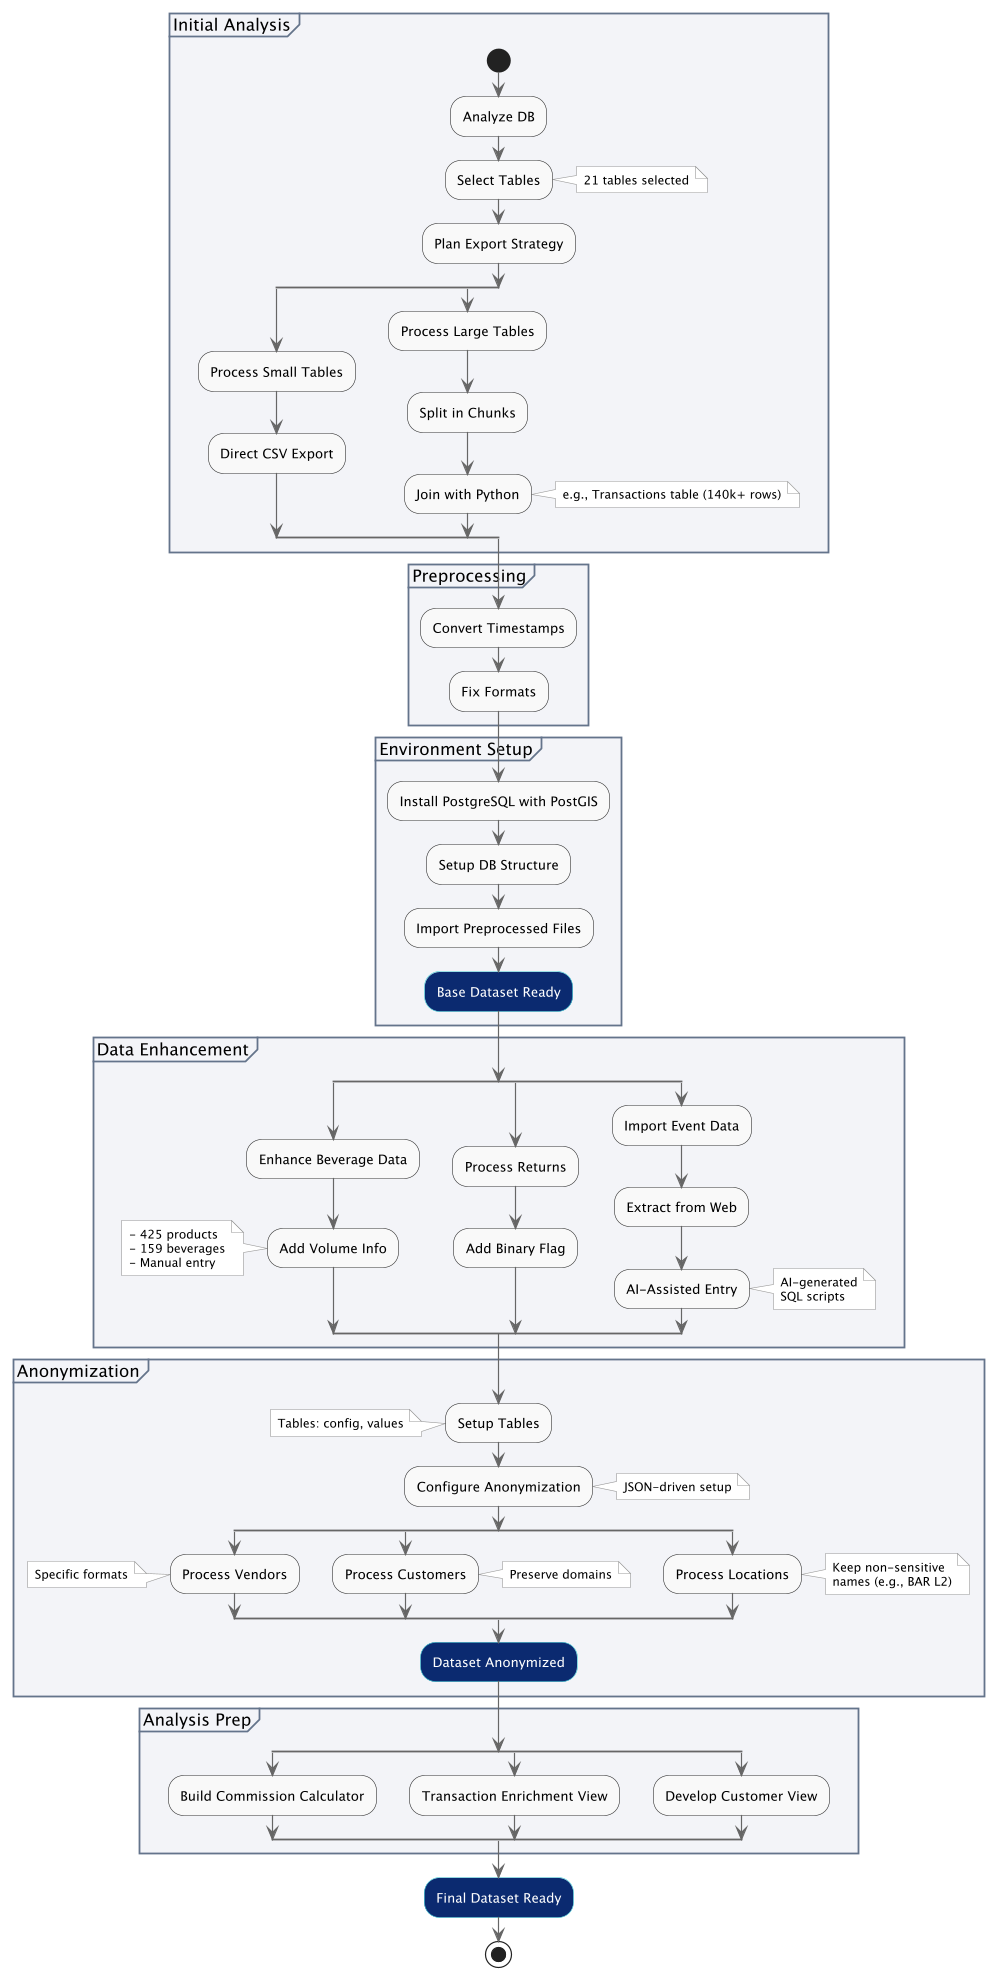
\includegraphics[width=0.8\textwidth]{\ThesisFigures/diagrams/kdd-workflow}
	\caption{Knowledge Data Discovery workflow diagram}
	\label{fig:data-methodology-diagram}
\end{figure}

	% ✅ chapter - data analysis and results
	%%% Data Analysis and Results
%%%%%%% Wording: ⏳
%%%%%%% Styling: ⏳
%%%%%%% References: ⏳
%%%%% Grammar: ⏳
%%% --------------------------------------------------------------
\chapter{Data Analysis and Results}
\label{ch:data-analysis-and-results}

This chapter presents the data analysis and results of the research.
The goal is to address the research questions outlined earlier, with a focus on providing actionable insights for the event organizer.

The chapter is divided into several sections corresponding to key analytical areas:\\
\begin{enumerate}
	\item \fullref{sec:analysis-cashflow-and-revenue-sources},
	\item \fullref{sec:analysis-performance-indicators},
	\item \fullref{sec:analysis-beverage-consumption},
	\item and~\fullref{sec:analysis-customers}
\end{enumerate}

Each section focuses on a different aspect of the data analysis trying to answer the research questions, present results, visualizations, and possible interpretations.

%%% Section: Cashflow and Revenue Sources Analysis
%%% --------------------------------------------------------------


\section{Cashflow and Revenue Sources Analysis}
\label{sec:analysis-cashflow-and-revenue-sources}

This section provides a comprehensive view of the festival's financial performance and cash flows.
It should answer critical questions about how finances were funded into the system, how were they processed, and what were the final outcomes.

For this analysis, four questions were previously formulated.
However, they were reordered to better fit the narrative of the analysis and logical flow of the chapter.

In the end, this section should provide a clear picture of the financial flows during the event and easy understanding of the generated revenue from various sources.

%%% Cashflow / Chip Top-Up Analysis
%%% --------------------------------------------------------------

\subsection{Chip Top-Up Analysis}
\label{subsec:analysis-chip-top-up}

\makerqbox{cashflow-top-up-balance}

Attendees could top up their chip balances via online prepayments or on-site using cash or card.
Additionally, the system allows to top-up~\enquote{artificial} credit for VIP-issued chips which is also a mean of funding the system.
However, these VIP credits are later not refundable, but this will be discussed in the next section.

This subsection quantifies these methods, highlighting their respective contributions to the overall top-up total.

To get the results, it was necessary to find all top-up transactions and their respective payment methods used.
This resulted in \bfmtnum{17704}~top-up transactions, with a total value of~\bfmtczk{14520973}.

When looking at the grouping by payment methods, the results in~\autoref{fig:top-up-transactions-by-payment-method} give a clear picture of the distribution.

\begin{figure}[H]
	\centering
	\small
	\begin{tabularx}{0.95\textwidth}{
		|>{\columncolor{unicorn_blue!5}}X
		|>{\columncolor{unicorn_blue!5}}r
		|>{\columncolor{unicorn_blue!5}}r|}
		\hline
		\rowcolor{unicorn_blue}
		\textbf{\color{white}Payment Method}
		& \textbf{\color{white}Count}
		& \textbf{\color{white}Total Value (CZK)} \\
		\hline
		\hline
		\colorindicator{1}Card terminal     & \fmtnum{8486}   & \fmtczk{7264503}   \\
		\colorindicator{2}Cash              & \fmtnum{7561}   & \fmtczk{5782570}   \\
		\colorindicator{3}Online pre top-up & \fmtnum{1634}   & \fmtczk{1436400}   \\
		\colorindicator{4}VIP issued        & \fmtnum{23}     & \fmtczk{37500}     \\
		\hline
		\hline
		\rowcolor{unicorn_blue!10}
		\textbf{Total}                      & \bfmtnum{17704} & \bfmtczk{14520973} \\
		\hline
	\end{tabularx}

	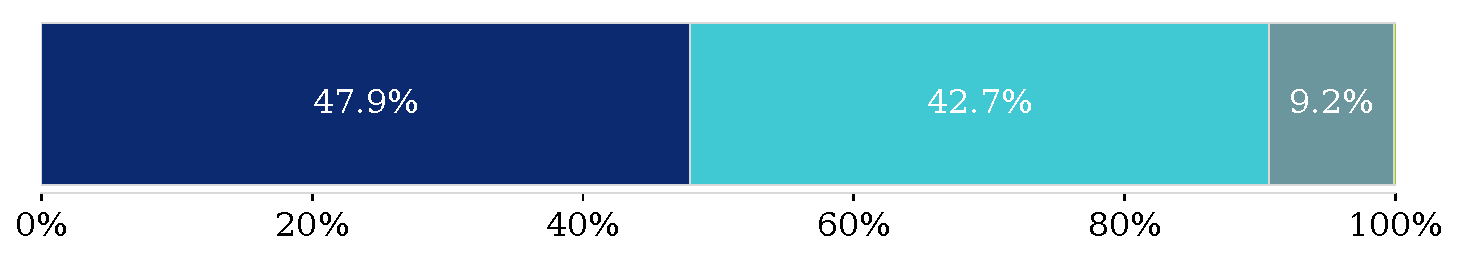
\includegraphics[width=\textwidth]{\ChartsDir/rq2-topup-methods}
	\caption{\rqshorttext{cashflow-top-up-balance} Top-Up Transactions by Payment Method}
	\label{fig:top-up-transactions-by-payment-method}
	\source
\end{figure}

Thanks to the results, it is clear how many funds did the system receive and by what means.

\begin{keytakeaways}
	\begin{itemize}
		\item The total top-up amount was~\bfmtczk{14520973}.
		\item The most used payment method was card terminal at the event with 50\% of all top-ups.
		\item Only around 10\% of the top-ups were done online.
	\end{itemize}
\end{keytakeaways}

%%% Cashflow / Sales Analysis
%%% --------------------------------------------------------------

\subsection{Sales Analysis}
\label{subsec:analysis-sales}

\makerqbox{cashflow-total-sales}

The sales analysis was crucial for understanding the overall sales behavior and served as a basis for further insights tightly connected to the revenue sources.

To answer the research question, it was necessary to find all sales transactions and their respective sellers and to divide them into two groups: the direct organizer's sales and external vendors' sales.
And for better understanding, the sales were also grouped by the product categories (see~\autoref{tab:product-categories} for the list of categories).

The results show that the total sales of the event were~\bfmtczk{11711807} with the organizer's sales being~\bfmtczk{8240264} and the external vendors' sales being~\bfmtczk{3471543}.

The organizer, most importantly, sold all the beer beverages and most of the non-alcoholic and alcoholic (spirits) beverages.
Whereas the external vendors sold mainly food, wine, beverages and other uncategorized products.
This can be seen in~\autoref{fig:sales-organizer-vs-vendors} below.

\begin{figure}[H]
	\centering
	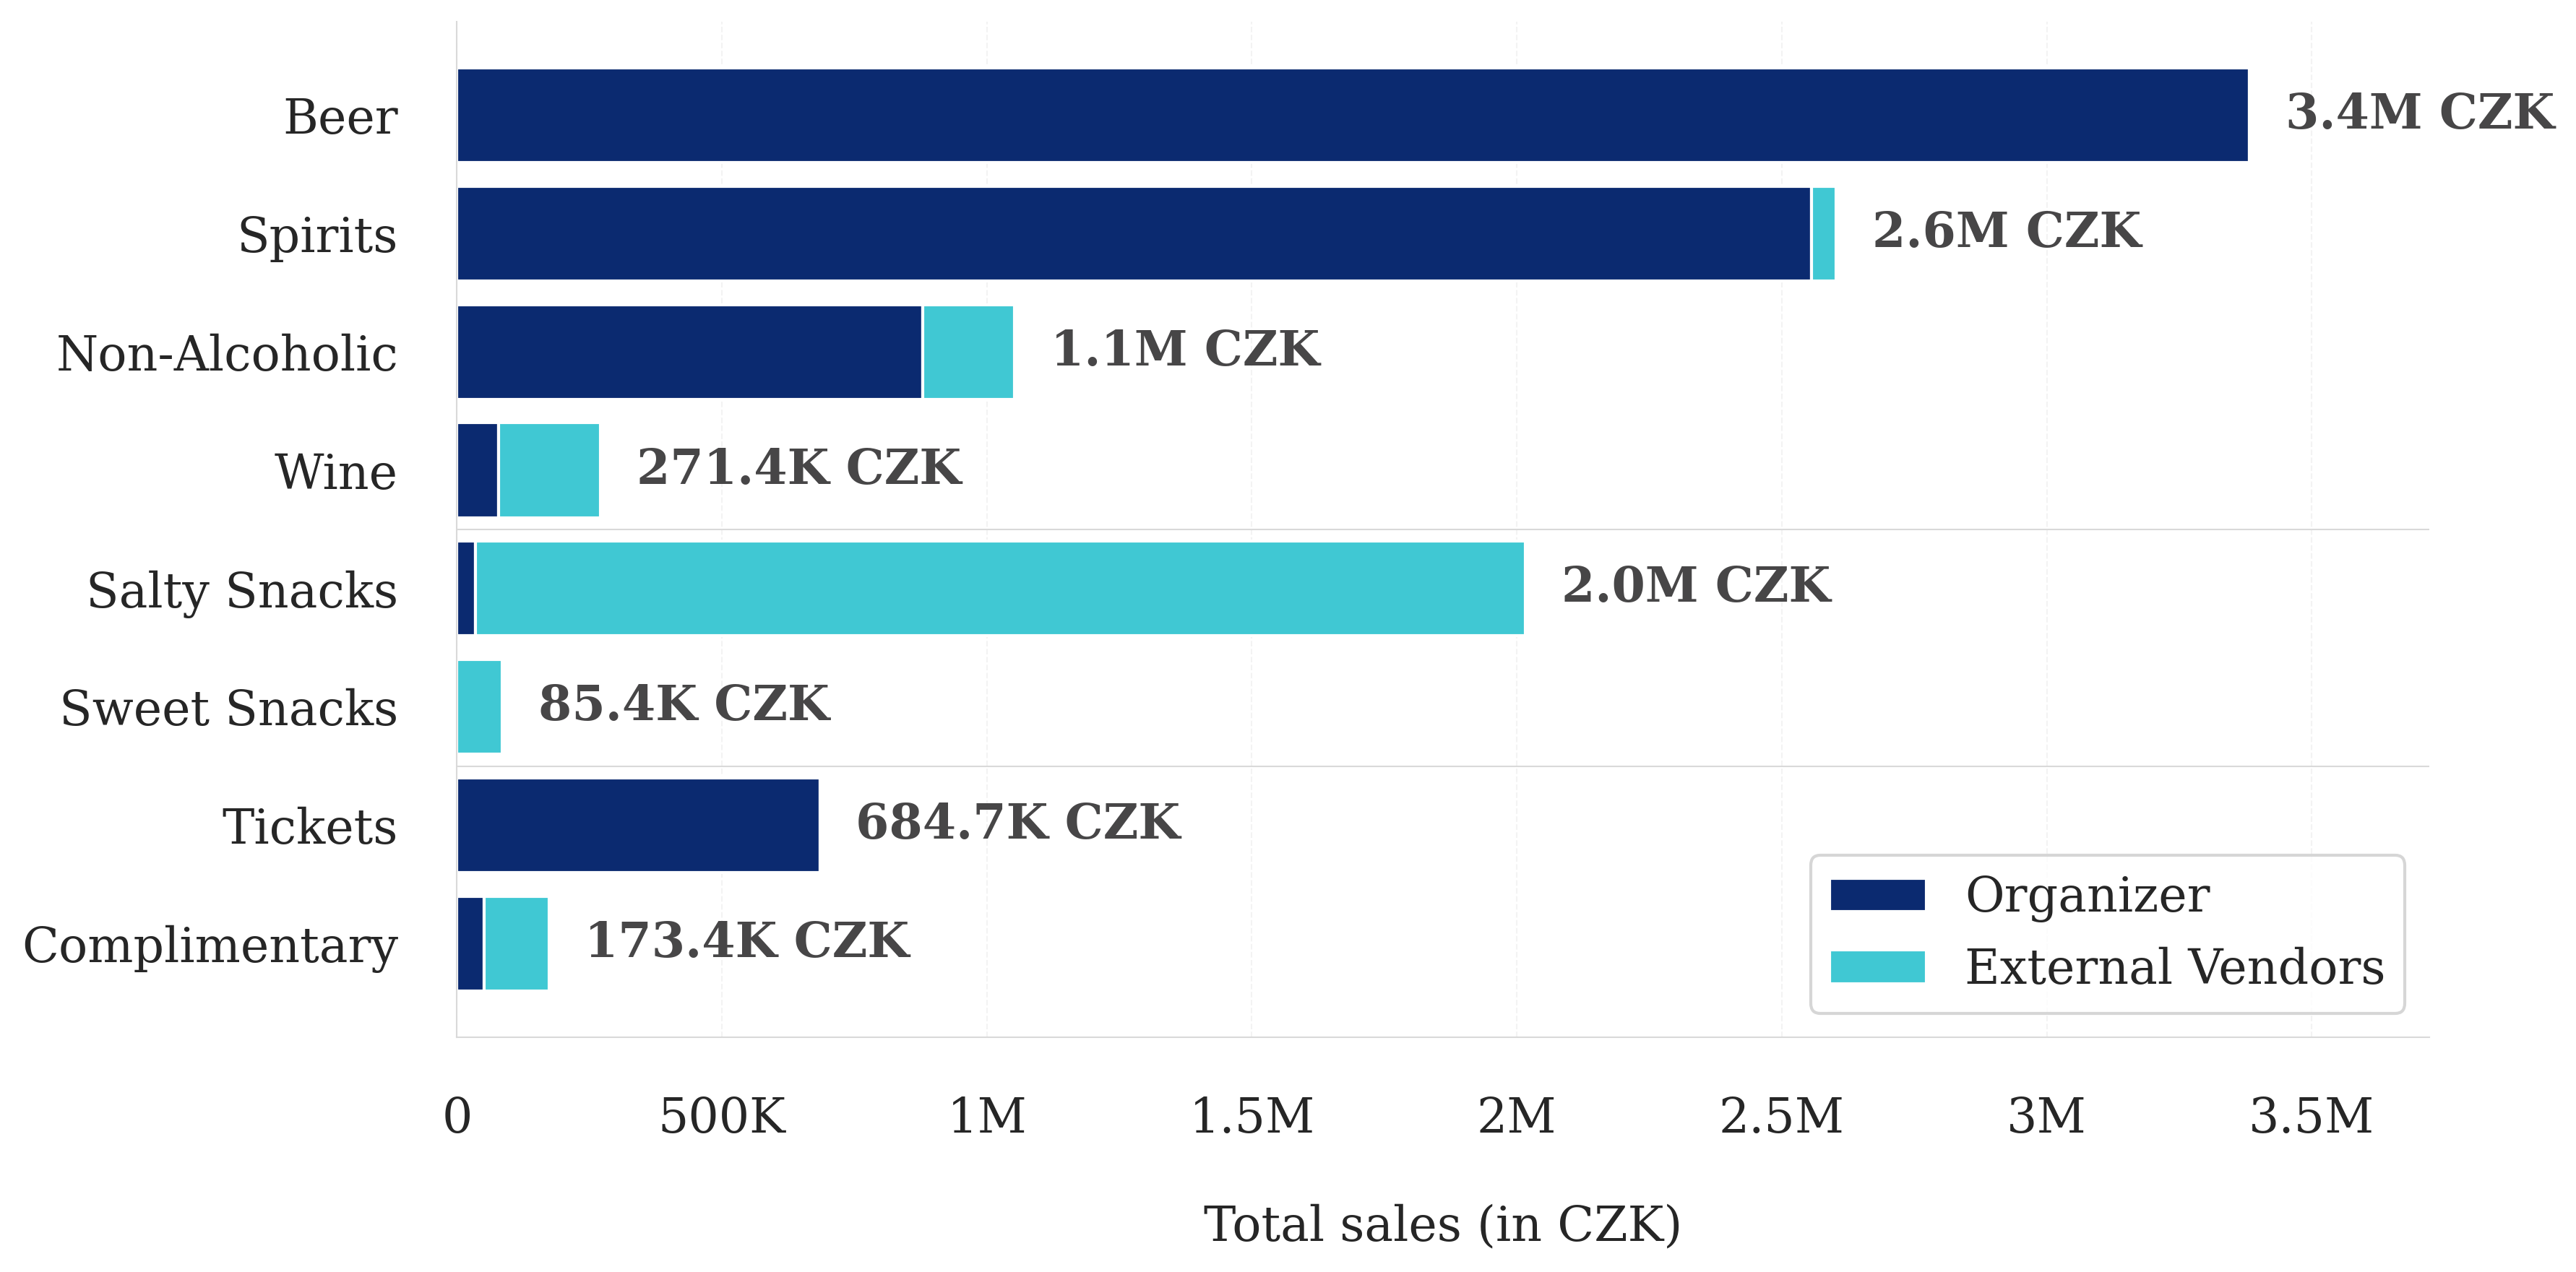
\includegraphics[width=\textwidth]{\ChartsDir/rq4-organizer-vs-vendor-sales}
	\caption{\rqshorttext{cashflow-total-sales} Sales of the Organizer vs. External Vendors}
	\label{fig:sales-organizer-vs-vendors}
	\source
\end{figure}

The organizer also sold not so little of uncategorized products, which after further investigation turned out to be ticket sales at the event amounting to~\bfmtczk{684700}.

In total, the organizer direct sales were \textbf{70\%} of the total sales, which is a significant portion, and thus the organizer itself has even bigger influence on the event's financial performance.

\begin{keytakeaways}
	\begin{itemize}
		\item Total sales of the event were~\bfmtczk{11711807}, where organizer sales were~\textbf{70\%} of the total.
		\item The organizer sold all beer beverages and the majority of the non-alcoholic and alcoholic beverages.
		\item The organizer also sold tickets at the event amounting to~\bfmtczk{684700}.
		\item External vendors sold food, wine, and other uncategorized products.
	\end{itemize}
\end{keytakeaways}


%%% Cashflow / Remaining Chip Balances
%%% --------------------------------------------------------------

\subsection{Remaining Chip Balances}
\label{subsec:analysis-remaining-balances}
\makerqbox{cashflow-remaining-balance}

The remaining chip balances are crucial for the event organizer as they represent the potential revenue that can be still claimed.
Any unclaimed balances after a given refund period, which is usually up to 14~days after the event will be considered as organizer's taxable revenue.

Out of the total top-up amount of~\bfmtczk{14520973}, the total spent credit amounted to~\bfmtczk{10984945}, which left a total of~\bfmtczk{3536028} on the chips before refunds.
After refunds – done both at the event (\bfmtczk{15379}) and later via online bank refund requests (\bfmtczk{3163567}) – the remaining balance was reduced to~\bfmtczk{357082}.

However, this still included the artificially issued VIP credits with leftover balance of~\bfmtczk{12405}.
The system also reported integrity errors in the data, which resulted in a total of~\bfmtczk{10246}~due to fraudulent activities performed by some attendees which were automatically suspended by the system.

This left the total unclaimed balance at~\bfmtczk{334431}, which has been claimed by the organizer as taxable revenue.

Since these numbers can be quite abstract, the results in a form of sankey diagram in~\autoref{fig:remaining-balances-sankey}~below provide a clear picture of the flow of the funds.

\begin{figure}[H]
	\centering
	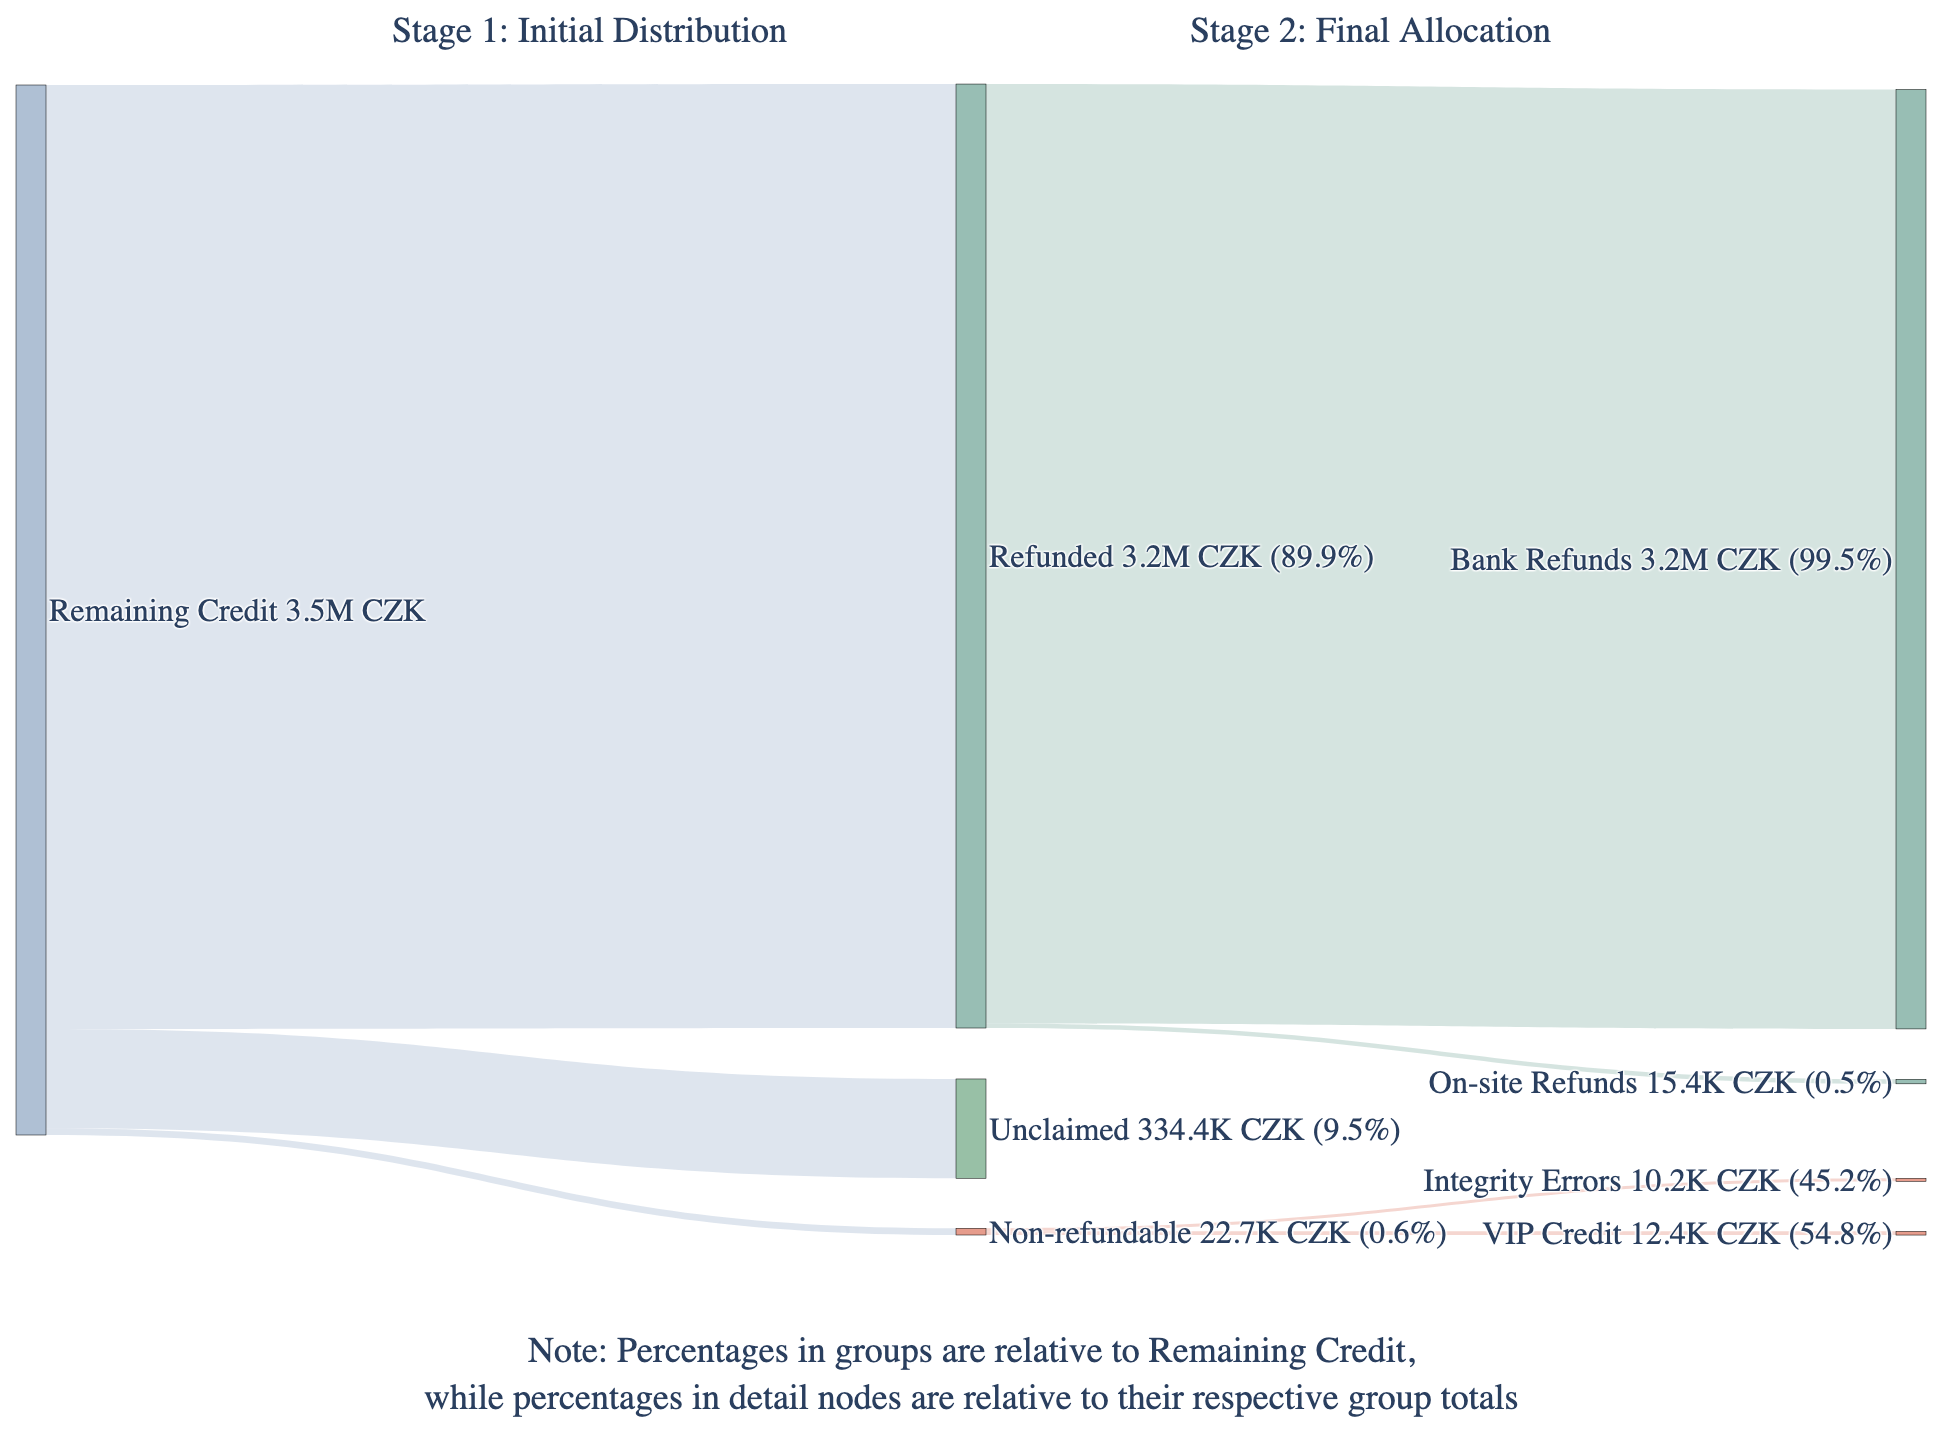
\includegraphics[width=\textwidth]{\ChartsDir/rq3-remaining-balances}
	\caption{\rqshorttext{cashflow-remaining-balance} Remaining Chip Balances Sankey Diagram}
	\label{fig:remaining-balances-sankey}
	\source
\end{figure}

Thanks to this breakdown, it is clear how the remaining balances were reduced and what was the final outcome.
These results are important for the last part of this section, which is the total revenue of the organizer.

\begin{keytakeaways}
	\begin{itemize}
		\item Total unused credit was~\bfmtczk{3536028}.
		\item Credit refunded to customers was~\bfmtczk{3178946}.
		\item After VIP issued credits and system integrity error, the unclaimed balance was~\bfmtczk{334431}.
	\end{itemize}
\end{keytakeaways}

%%% Cashflow / Total Revenue of the Organizer
%%% --------------------------------------------------------------

\subsection{Total Revenue of the Organizer}
\label{subsec:analysis-total-revenue}
\makerqbox{cashflow-total-revenue}

The festival's financial model is based on a combination of revenue streams.

The most important stream is the \textbf{commission from the vendor sales}, which is arranged in advance between the organizer and the vendors.
The commission is, in this case, a percentage (ranging from 15\% to 30\% depending on the deal) of the vendor sales amount without VAT\@.

Therefore, this required finding all sales transactions made at the external vendors' stands and calculating the commission based on the agreed percentage.
However, this was not a straightforward task, since a transaction could contain multiple products even from different vendors.

This required a more complex calculation, for which was used the previously mentioned data processing views which were designed for this purpose.
In the end, the total revenue from sales commissions was~\bfmtczkp[2]{820712,79}.

Another source of revenue is the \textbf{unclaimed chip balances}, which, after a credit refund period, are considered as taxable revenue for the organizer.
This, thanks to the previous subsection, was found to be~\bfmtczk{334431}.

Currently totalling~\bfmtczkp[2]{1155143,79} is the direct revenue of the organizer from the event.
However, given the circumstances and setup of this event, there were also additional, but indirect revenue streams that were not included in the total revenue.
These include \textbf{the online ticket sales}, which were sold by the organizer and \textbf{the direct sales of the organizer}.
They were not included in the total direct revenue, as they may misinterpret the results since the analysis lacks expenses of the organizer.

If we were to include these, the total revenue would increase by~\bfmtczk{11179700} from the online ticket sales and~\bfmtczk{8240264} from the direct sales, which would result in a total revenue of~\bfmtczkp[2]{20575107,79}.

To better understand the revenue streams, the results are visualized in~\autoref{fig:revenue-breakdown-total}~below.

\begin{figure}[H]
	\centering
	% chart
	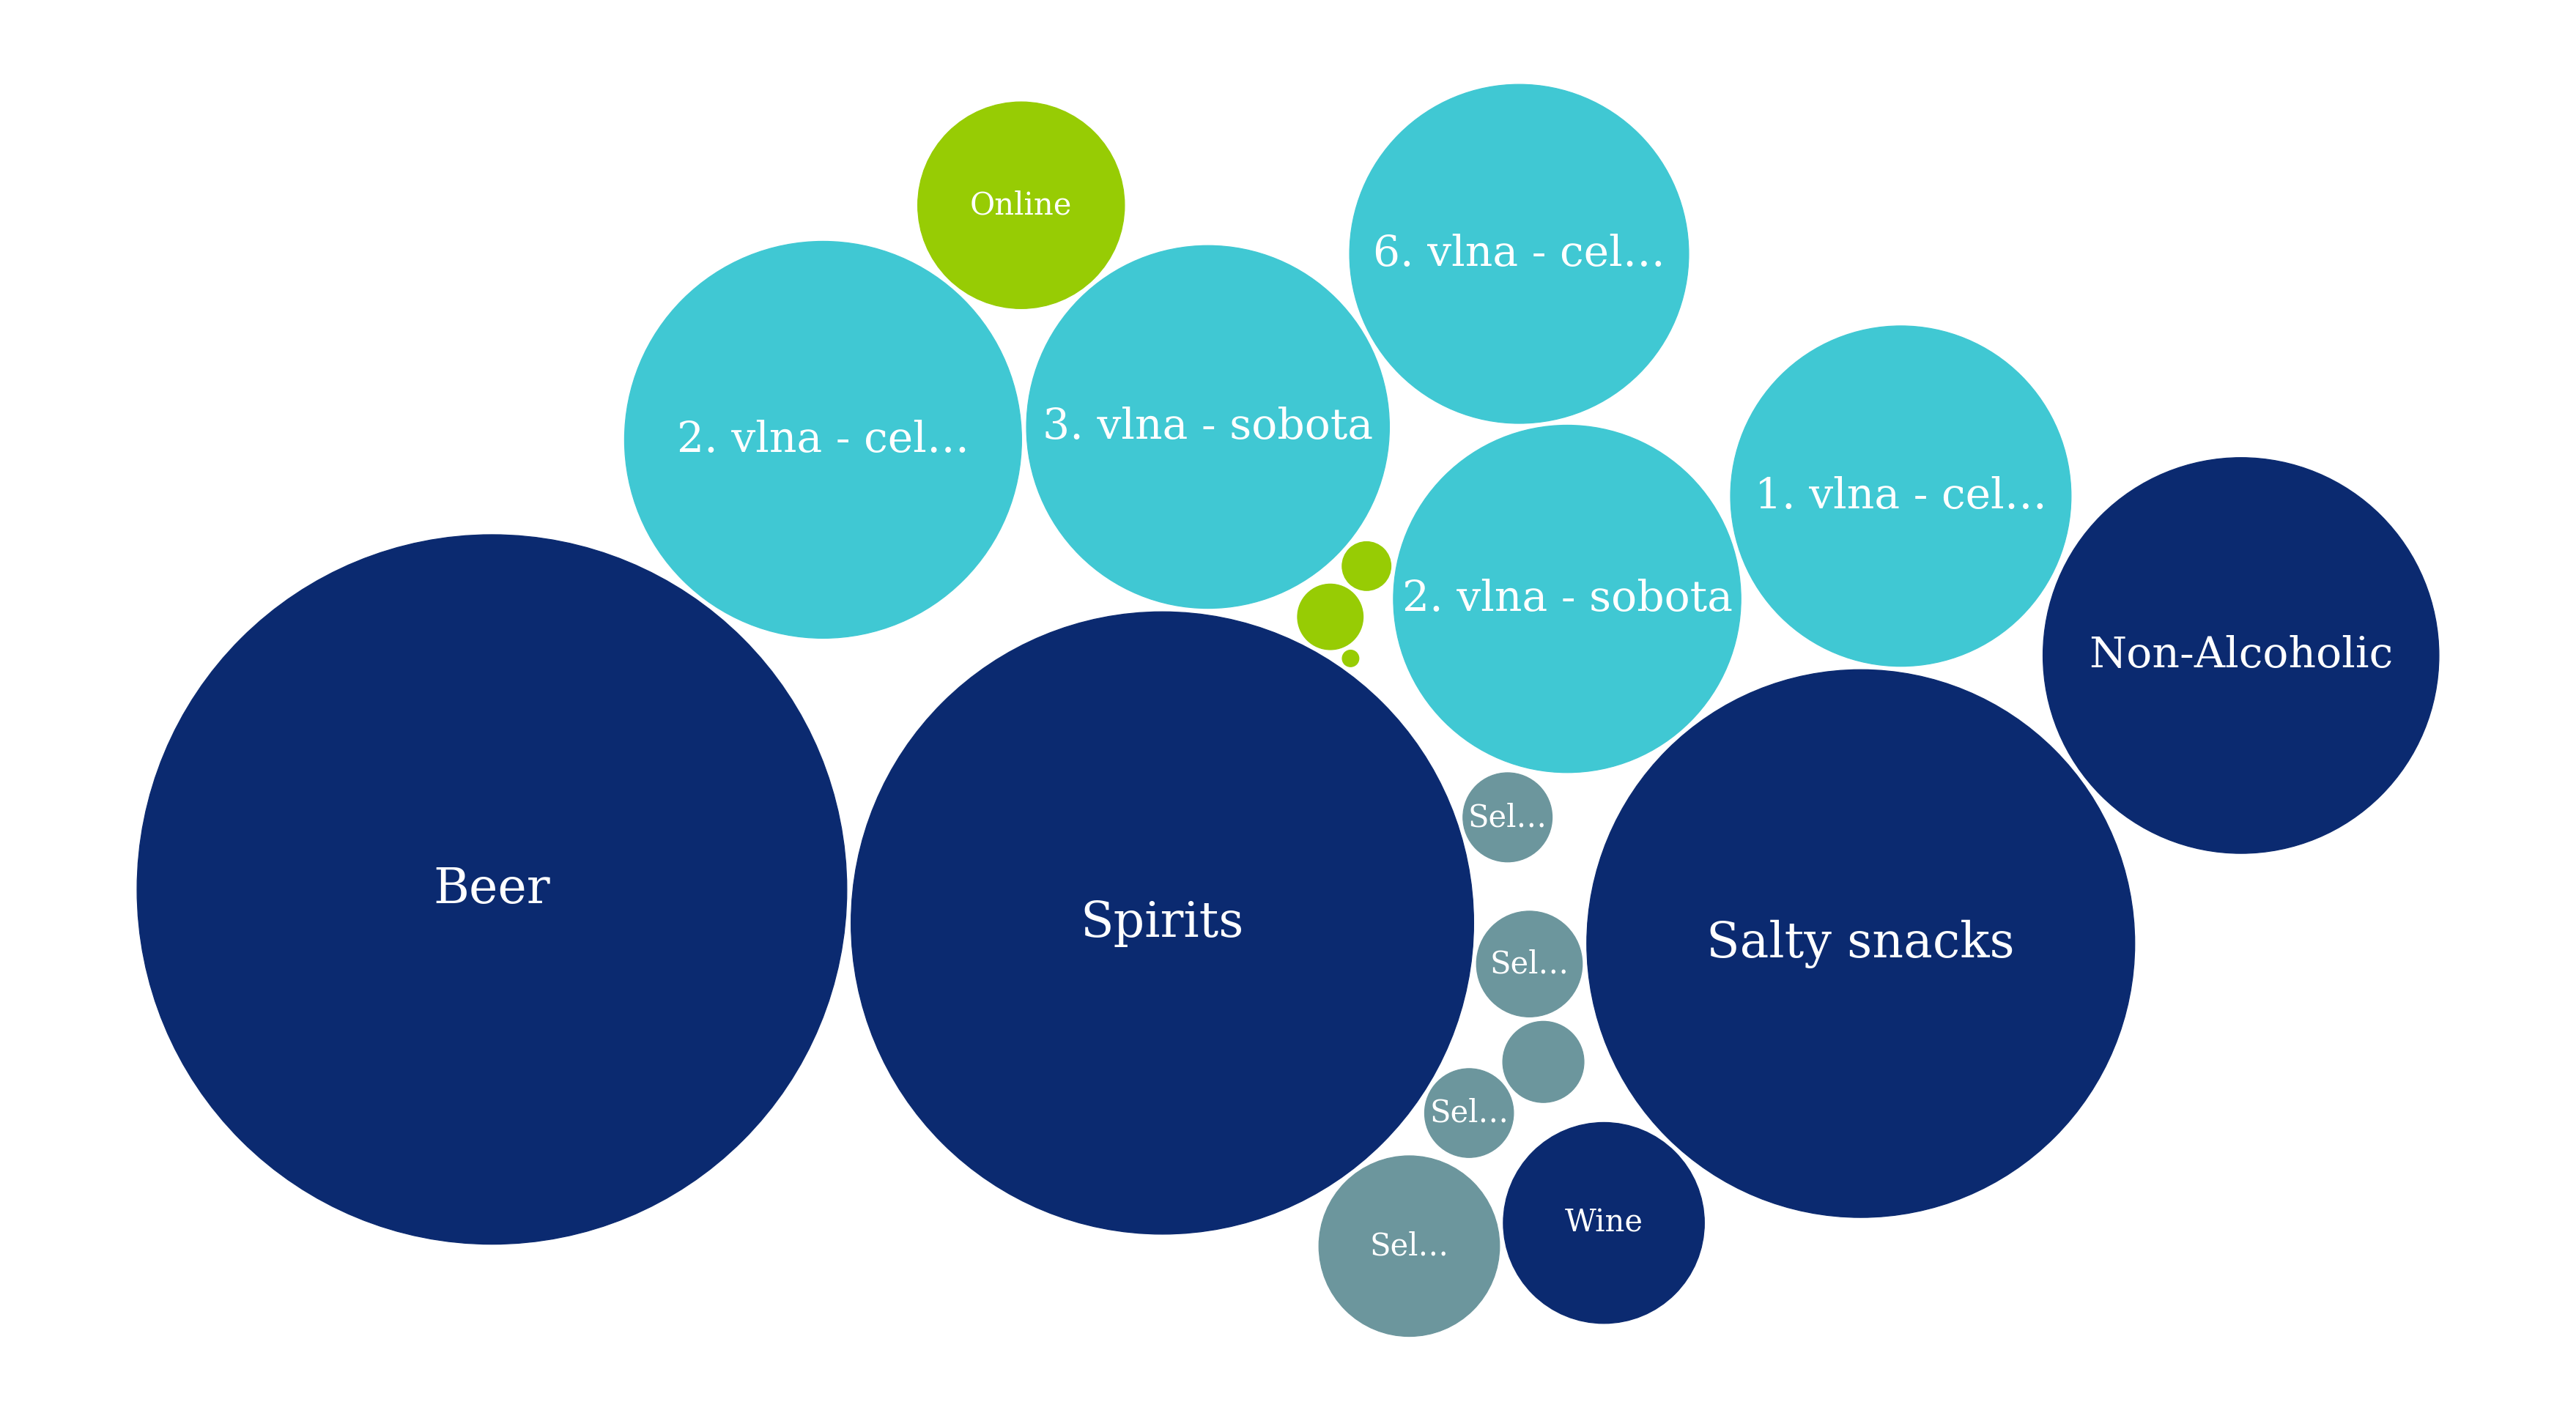
\includegraphics[width=\textwidth]{\ChartsDir/rq1-total-revenue-breakdown}
	% space
	\par\vspace*{0.5em}
	% table
	\begin{tabularx}{\textwidth}{|>{\columncolor{unicorn_blue!5}}X|>{\columncolor{unicorn_blue!5}}r|}
		\hline
		\rowcolor{unicorn_blue}
		\textbf{\color{white}Revenue Stream}    & \textbf{\color{white}Amount} \\
		\hline
		\hline
		\colorindicator{3}Vendor Commissions      & \fmtczkp[2]{820712.79}       \\
		\colorindicator{4}Unclaimed Chip Balances & \fmtczk{334431}              \\
		\hline
		\textbf{Total Direct Revenue}             & \bfmtczkp[2]{1155143.79}     \\
		\hline
		\colorindicator{2}Online Ticket Sales     & \fmtczk{11179700}            \\
		\colorindicator{1}Organizer Direct Sales  & \fmtczk{8240264}             \\
		\hline
		\textbf{Total Revenue (All Streams)}      & \bfmtczkp[2]{20575107.79}    \\
		\hline
	\end{tabularx}
	\caption{\rqshorttext{cashflow-total-revenue} Breakdown of All Revenue Streams}
	\label{fig:revenue-breakdown-total}
	\source
\end{figure}

\begin{keytakeaways}
	\begin{itemize}
		\item Total direct revenue of the organizer was~\bfmtczkp[2]{1155143,79}.
		\item Vendor sale commission contributed to~approximately 71\% of the total direct revenue.
		\item With other indirect revenue streams, the total revenue would be~\bfmtczkp[2]{20575107,79}.
	\end{itemize}
\end{keytakeaways}

%%% Cashflow / Summary
%%% --------------------------------------------------------------

\subsection{Summary}
\label{subsec:analysis-cashflow-summary}

This section provided a comprehensive view of the festival's financial performance and cash flows.
The results covered the top-up transactions, sales analysis, remaining chip balances, and the total revenue of the organizer and contributed to a better understanding from the financial perspective of the festival.

Nevertheless, results covered in these subsections are only a part of the whole picture and can be interpreted in various ways.

For this particular challenge, a summarized cash flow diagram of payments was created, containing thus only the direct revenue streams.
This diagram can be seen in the~\autoref{fig:cash-flow-diagram} below.

\begin{figure}[H]
	\centering
	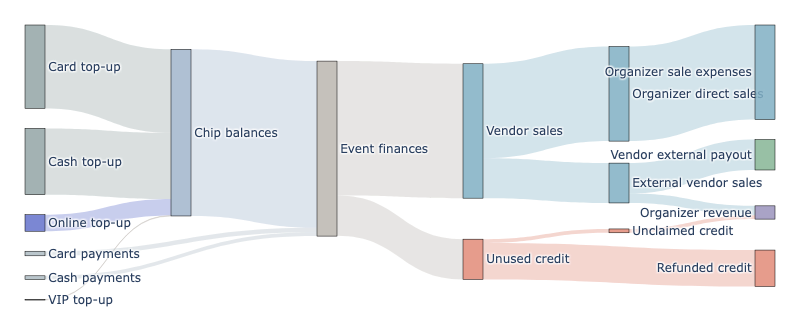
\includegraphics[width=0.95\textwidth]{\ThesisFigures/charts/revenue-cash-flows}
	\caption{Overall Cash Flow Diagram}
	\label{fig:cash-flow-diagram}
	\source
\end{figure}

This diagram provides a clear overview of the financial flows during the festival and nicely summarizes the results of this analysis.

% TODO: summarize
\begin{keytakeaways}
	\begin{itemize}
		\item Total incoming money flow was~\bfmtczk{14520973} from top-up transactions and~\bfmtczk{726862} from non-chip sales.
		\item Total sales amounted to~\bfmtczk{11711807}.
		\item This left a total of~\bfmtczk{3536028}~in unused credit before refunds.
		\item After refunds and non-refundable chips, the remaining balance left was~\bfmtczk{334431} claimed as taxable revenue.
		\item Commission from external vendor sales contributed to~\bfmtczkp[2]{820712,79}~of the total direct revenue.
		\item Together, the total direct revenue of the organizer was~\bfmtczkp[2]{1155143,79}.
	\end{itemize}
\end{keytakeaways}

%%% Section: Performance Indicators Analysis
%%% --------------------------------------------------------------


\section{Performance Indicators Analysis}
\label{sec:analysis-performance-indicators}

% TODO: rephrase
This section focuses on the performance indicators of the event.
The goal is to identify key metrics that can be used to further evaluate the event and its success.
The potential of this analysis is to measure the~\enquote{greatness}~and the size of the event in terms of performance.

This analysis aims to provide answers to previously defined research questions about the event's performance.
For the purpose of this analysis, they were slightly reordered and grouped into the two subsections listed below:
\begin{enumerate}
	\item \fullref{subsec:analysis-performance-indicators-transactions}
	\item and~\fullref{subsec:analysis-performance-indicators-best}
\end{enumerate}

The results of this analysis should provide insights into the event's performance and help the organizer to understand the key metrics that can be used to evaluate the event's success.

%%% Performance / Transactions Processing Analysis
%%% --------------------------------------------------------------

\subsection{Transactions Processing Analysis}
\label{subsec:analysis-performance-indicators-transactions}

This subsection will focus on the processing of transactions during the event in pursuit of answering the three first research questions of this section.

\makerqbox{performance-transactions}

This question actually consists of two sub-questions, which will be addressed separately.

The first part questions the total number of transactions processed during the event.
This was actually quite simple to answer, as the system was designed to track all transactions and their types.
The resulted total number of transactions was~\bfmtnum{141381} consisting of~\bfmtnum{110854}~sales transactions, \bfmtnum{17726}~top-up transactions and~\bfmtnum{12801}~chip register transactions.

The second part focuses on rather time-related metrics and asks about the processing peak times during the festival.
For this part, it was necessary to spread out the above transactions over time and find the peaks.

The results in the~\autoref{fig:transactions-peaks} below show the distribution of the processed transactions over time.
It clearly identifies the peak on the last day of the festival at 18:00 amounting to~\bfmtnum{8986}~transactions.

\begin{figure}[H]
	\centering
	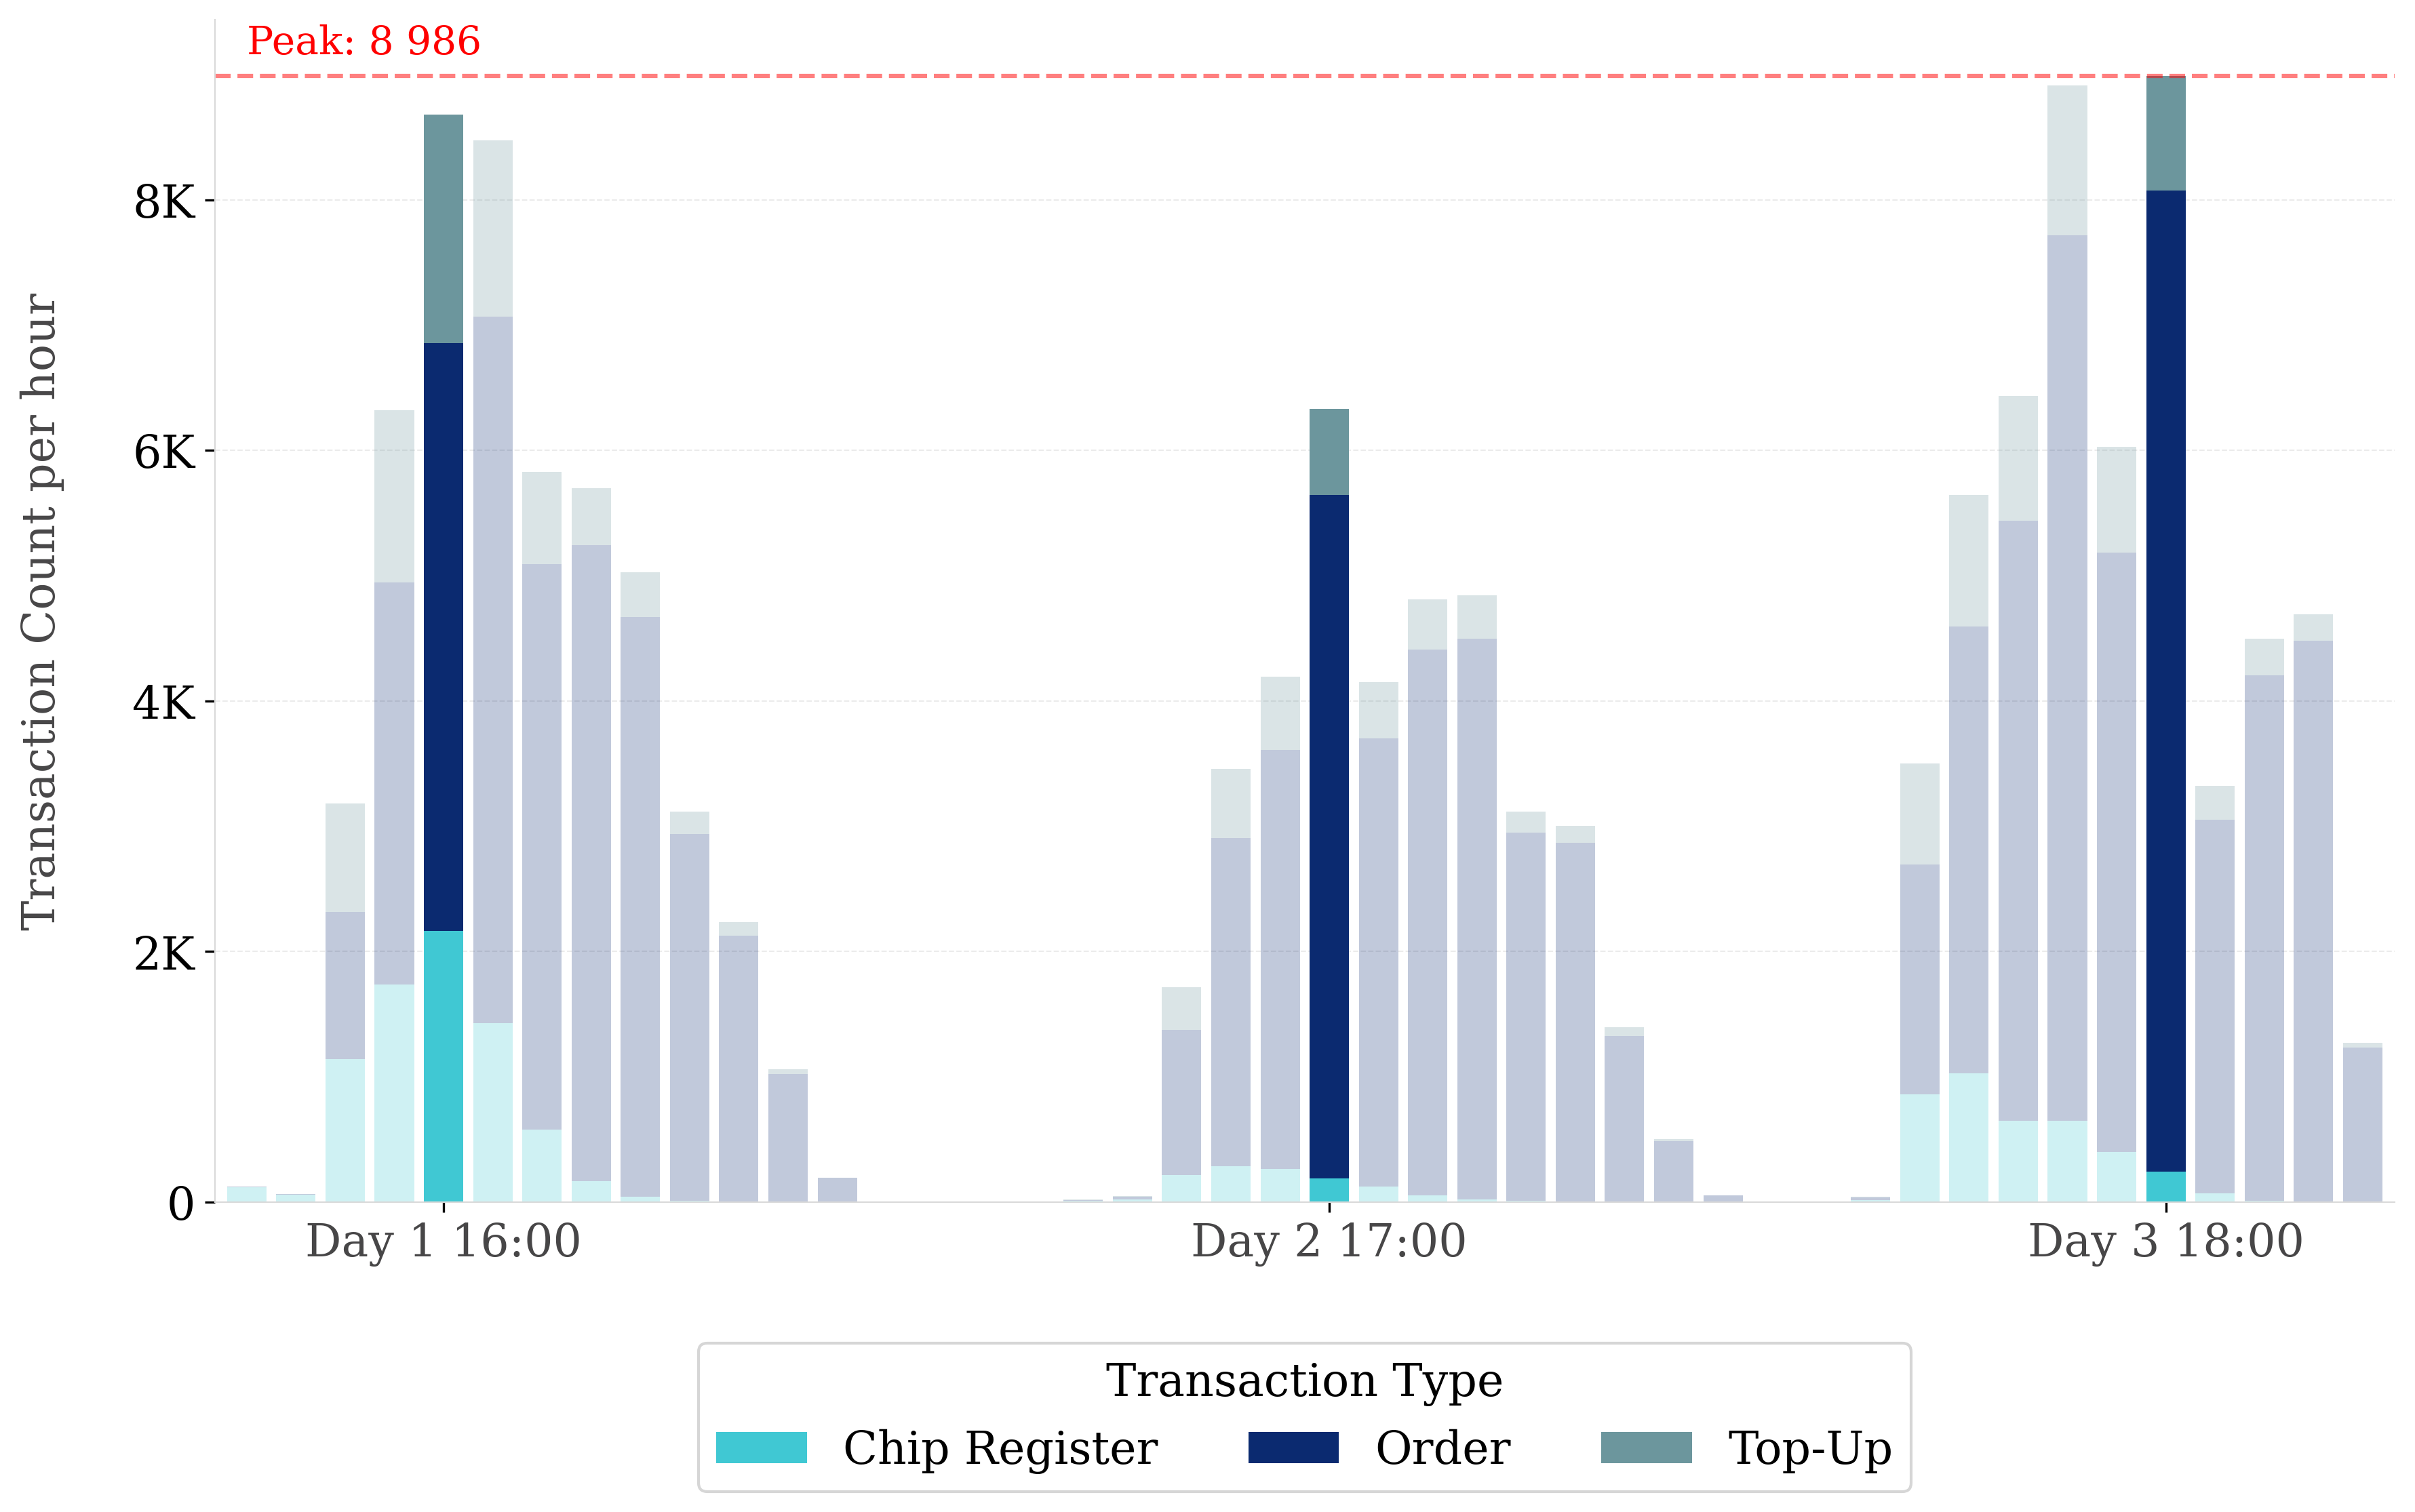
\includegraphics[width=\textwidth]{\ChartsDir/rq5-transaction-peaks}
	\caption{\rqshorttext{performance-transactions} Transactions Peaks}
	\label{fig:transactions-peaks}
	\source
\end{figure}

\begin{keytakeaways}
	\begin{itemize}
		\item Total number of transactions processed was~\bfmtnum{141381} consisting mainly (\bfmtnum{78}\%) of order transactions.
		\item The peak of transactions was on the last day of the festival at 18:00 with~\bfmtnum{8986}~transactions processed at that hour.
	\end{itemize}
\end{keytakeaways}

The following two questions (\rqshort{performance-processing-during-peaks}~and~\rqshort{performance-delays-downtimes}), focus on processing times and potential delays during the event.

\makerqbox{performance-processing-during-peaks}

The answer to this question is closely related to the previous one, as it requires the identification of the processing times during the peak times, which were already identified.

It required finding the average processing time, meaning difference between the transaction creation and its completion times.

\begin{infobox}{What causes the processing time?}
	Time when the transaction is created is the time when the in-place offline-supported system created the transaction, and the processed time is later when the central system receives the transaction and processes it.

	The delays can be caused by various factors, such as network latency, offline mode active, system load, or even the transaction type.
\end{infobox}

The results show that the average processing time during the peak times was approximately~\bfmtnum{47}~seconds.

When slightly changing the displayed data, we also get the answer to the~\rqshort{performance-delays-downtimes} about the potential delays and downtimes during the event.

\makerqbox{performance-delays-downtimes}

The chart in the~\autoref{fig:rq7-processing-times}~shows the distribution of the processing times over the time and identifies one high processing peak of approximately~\bfmtnum{11}~minutes.
This is highly unusual and indicates a vendor misuse of the system or accidentally put the system into offline mode.

\begin{figure}[H]
	\centering
	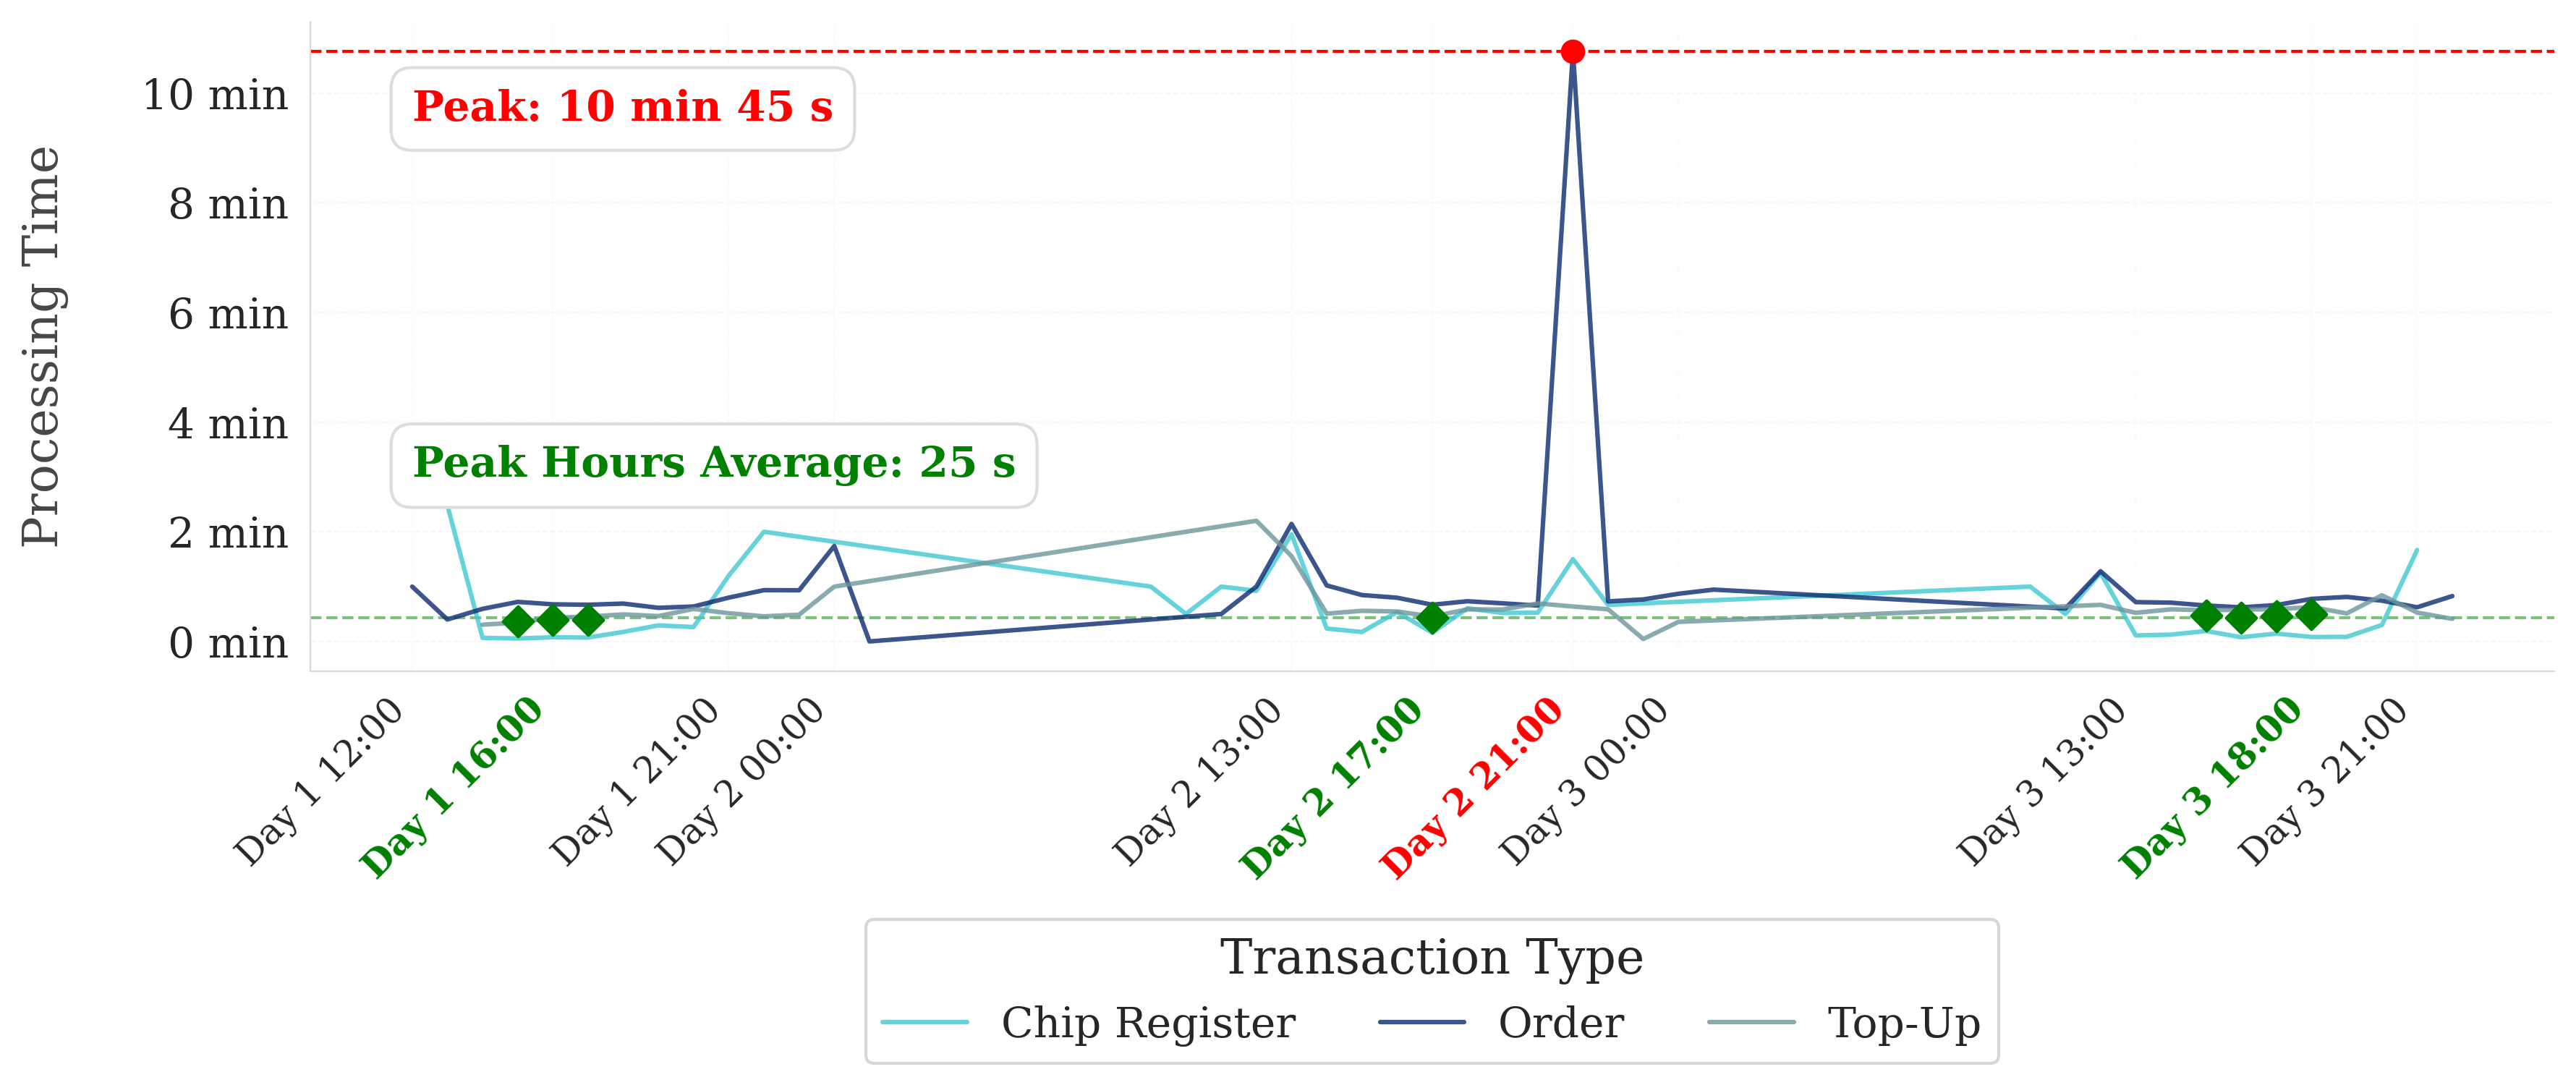
\includegraphics[width=\textwidth]{\ChartsDir/rq7-processing-times}
	\caption{\rqshorttext{performance-delays-downtimes} Transaction Processing Times}
	\label{fig:rq7-processing-times}
	\source
\end{figure}

Other high peaks are visible on the second day in the afternoon with approximately~\bfmtnum{3}~minutes processing time, which was probably caused by the initial load on that day.

\begin{keytakeaways}
	\begin{itemize}
		\item The average processing time during the peak times was~\bfmtnum{47}~seconds.
		\item The highest processing peak was approximately~\bfmtnum{11}~minutes, indicating a potential misuse of the system.
		\item Other high peaks were visible on the second day in the afternoon with approx.\~\bfmtnum{3}~minutes processing time.
	\end{itemize}
\end{keytakeaways}

These results provide insights into the system's performance during the event, its reliability, and potential bottlenecks.
It also shows the festival's popularity and the system's ability to handle the load.

%%% Performance / Best Sale & Top-Up Points, Vendors, and Products Analysis
%%% --------------------------------------------------------------

\subsection{Best Sale \& Top-Up Points, Vendors, and Products Analysis}
\label{subsec:analysis-performance-indicators-best}
In this subsection, the main goal will be to address the last four research questions of this section and provide insights into the best: selling points, top-up points, vendors, and products.

The problem with these question statements is that they are quite broad and can be interpreted in various ways.
What does a~\enquote{best} mean in this context?

It can be the most profitable, the best rated, the most visited, etc.
But since we are exploring the performance indicators, the best should be understood as the~\enquote{busiest}.
In terms of the system and this analysis, it should mean \textbf{the most transactions created} and possibly the point's ability to handle the load.

%%% Performance / Best Sale & Top-Up Points, Vendors, and Products Analysis / Best Sale Points
%%% --------------------------------------------------------------

\subsubsection{Best Top-Up Points}
\label{subsubsec:analysis-best-top-up-points}

The first focus will be on the best top-up points since unlike the selling points, vendors and products, the top-up points are not linked to any specific product or vendor.

\makerqbox{performance-best-top-up-points}

To find these results, it required finding all top-up transactions, aggregate them in a bucket-like time frame and finally calculate their total counts, max peaks and averages over time.

This resulted in the following findings in the~\autoref{tab:best-topup-points} below.

\begin{table}[htbp]
	\centering
	\small
	\begin{tabularx}{\textwidth}{
		|>{\columncolor{unicorn_blue!5}\centering\arraybackslash}p{1cm}
		|>{\columncolor{unicorn_blue!5}\raggedright\arraybackslash}X
		|>{\columncolor{unicorn_blue!5}\raggedleft\arraybackslash}p{2.5cm}
		|>{\columncolor{unicorn_blue!5}\raggedleft\arraybackslash}p{2.5cm}
		|>{\columncolor{unicorn_blue!5}\raggedleft\arraybackslash}p{2.5cm}|}
		\hline
		\rowcolor{unicorn_blue}
		\textbf{}
		& \textbf{\color{white}Top-Up point}
		& \textbf{\color{white}Customers}
		& \textbf{\color{white}Transactions}
		& \textbf{\color{white}Max trx./h}
		\\\hline\hline
		% first rows
		\csvreader[
		head to column names,
		late after line={\\\hline},
		filter={\thecsvinputline<6}
		]{\DataDir/rq9-best-topup-points.csv}{
			entity=\colentity,
			customer_count=\colcustomers,
			transaction_count=\coltrxcount,
			max_hourly_peak=\colhourlypeak
		}{
			\the\numexpr\thecsvinputline-1
			& \colentity
			& \num[group-separator={,}]{\colcustomers}
			& \num[group-separator={,}]{\coltrxcount}
			& \num[group-separator={,}]{\colhourlypeak}
		}
		% separator
		\noalign{\vspace{1mm}}
		\multicolumn{5}{c}{\footnotesize{\textellipsis}}
		\\
		\noalign{\vspace{1mm}}
		\hline
		% middle rows
		\csvreader[
		head to column names,
		late after line={\\\hline},
		filter={\thecsvinputline>15 \AND \thecsvinputline<20}
		]{\DataDir/rq9-best-topup-points.csv}{
			entity=\colentity,
			customer_count=\colcustomers,
			transaction_count=\coltrxcount,
			max_hourly_peak=\colhourlypeak
		}{
			\the\numexpr\thecsvinputline-1
			& \colentity
			& \num[group-separator={,}]{\colcustomers}
			& \num[group-separator={,}]{\coltrxcount}
			& \num[group-separator={,}]{\colhourlypeak}
		}
		% separator
		\noalign{\vspace{1mm}}
		\multicolumn{5}{c}{\footnotesize{\textellipsis}}
		\\
		\noalign{\vspace{1mm}}
		\hline
		% last rows
		\csvreader[
		head to column names,
		late after line={\\\hline},
		filter={\thecsvinputline>25}
		]{\DataDir/rq9-best-topup-points.csv}{
			entity=\colentity,
			customer_count=\colcustomers,
			transaction_count=\coltrxcount,
			max_hourly_peak=\colhourlypeak
		}{
			\the\numexpr\thecsvinputline-1
			& \colentity
			& \num[group-separator={,}]{\colcustomers}
			& \num[group-separator={,}]{\coltrxcount}
			& \num[group-separator={,}]{\colhourlypeak}
		}
	\end{tabularx}
	\caption{\rqshorttext{performance-best-top-up-points} Best Top-Up Points}
	\label{tab:best-topup-points}
\end{table}

This indicates that the most busy top-up points were somehow evenly distributed with approximately around \textbf{1000~transactions} processed during the event with average peaks of around \textbf{100~transactions/hour}.
The least busy top-up points were the specific ones, such as the Support tent, VIP and Accreditation points, which were not used so much for top-ups.

The overall distribution, shown in the~\autoref{fig:best-topup-points}, also shows that Top-up points were more busy than Check-in points.
That makes sense because the top-ups were done more frequently than the initial check-ins, but the check-ins were done in a more concentrated time frame.

\begin{figure}[H]
	\centering
	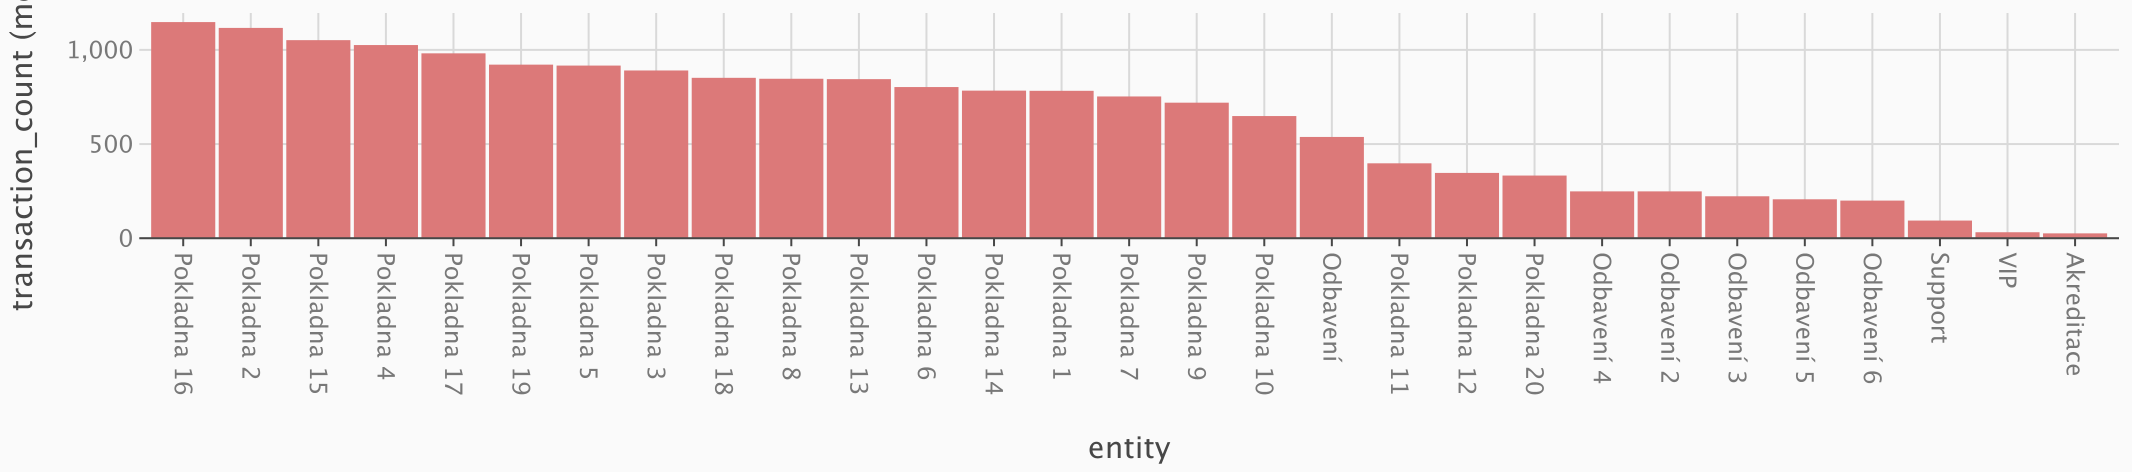
\includegraphics[width=\textwidth]{\ChartsDir/rq9-best-topup-points}
	\caption{\rqshorttext{performance-best-top-up-points} Best Top-Up Points}
	\label{fig:best-topup-points}
	\source
\end{figure}

Especially \textbf{Odbavení} point processed only~\bfmtnum{529}~transactions but peaked at~\bfmtnum{125}~transactions per hour, which was much higher than the other check-in points and even higher than the best top-up points.

% TODO: summarize
\begin{keytakeaways}
	\begin{itemize}
		\item The most busy top-up points processed around~\bfmtnum{1000}~transactions during the event.
		\item The average peak of the top-up points was around~\bfmtnum{100}~transactions per hour.
		\item The least busy top-up points were the specific ones, such as the Support tent, VIP and Accreditation points.
		\item Check-in points were less busy than the top-up points, but the \textbf{Odbavení} point peaked at~\bfmtnum{125}~transactions per hour.
	\end{itemize}
\end{keytakeaways}

%%% Performance / Best Sale & Top-Up Points, Vendors, and Products Analysis / Best Sale Points
%%% --------------------------------------------------------------

\subsubsection{Best Sale Points}
\label{subsubsec:analysis-best-sale-points}

The next focus will be on the best sale points, which are the points where the most orders were created.

\makerqbox{performance-best-sale-points}

The process of finding the best sale points was similar to the previous one, but this time it required finding all sales transactions and their respective points.

Out of total of~\bfmtnum{145}~sale points, the best place was undeniable the \textbf{L20 PIVNÍ STAN 1} with total~\bfmtnum{10114}~orders processed and the maximum peak of~\bfmtnum{840}~orders per hour.

Another interesting fact is the number of unique users processed at the places.
The \textbf{L20 PIVNÍ STAN 1} processed~\bfmtnum{9159}~unique customers, accounting for a significant portion (\bfmtnump[2]{91.50}{}\%) of the total.

\begin{table}[htbp]
	\centering
	\small
	\begin{tabularx}{\textwidth}{
		|>{\columncolor{unicorn_blue!5}\centering\arraybackslash}p{1cm}
		|>{\columncolor{unicorn_blue!5}\raggedright\arraybackslash}X
		|>{\columncolor{unicorn_blue!5}\raggedleft\arraybackslash}p{2.5cm}
		|>{\columncolor{unicorn_blue!5}\raggedleft\arraybackslash}p{2.5cm}
		|>{\columncolor{unicorn_blue!5}\raggedleft\arraybackslash}p{2.5cm}|}
		\hline
		\rowcolor{unicorn_blue}
		\textbf{}
		& \textbf{\color{white}Sale Point}
		& \textbf{\color{white}Customers}
		& \textbf{\color{white}Orders}
		& \textbf{\color{white}Max orders./h}
		\\\hline\hline
		% first rows
		\csvreader[
		head to column names,
		late after line={\\\hline},
		filter={\thecsvinputline<9}
		]{\DataDir/rq8-best-sale-points.csv}{
			entity=\colentity,
			customer_count=\colcustomers,
			transaction_count=\coltrxcount,
			max_hourly_peak=\colhourlypeak
		}{
			\the\numexpr\thecsvinputline-1
			& \colentity
			& \num[group-separator={,}]{\colcustomers}
			& \num[group-separator={,}]{\coltrxcount}
			& \num[group-separator={,}]{\colhourlypeak}
		}
		% separator
		\noalign{\vspace{1mm}}
		\multicolumn{5}{c}{\footnotesize{\textellipsis}}
		\\
		\noalign{\vspace{1mm}}
		\hline
		% last rows
		\csvreader[
		head to column names,
		late after line={\\\hline},
		filter={\thecsvinputline>132}
		]{\DataDir/rq8-best-sale-points.csv}{
			entity=\colentity,
			customer_count=\colcustomers,
			transaction_count=\coltrxcount,
			max_hourly_peak=\colhourlypeak
		}{
			\the\numexpr\thecsvinputline-1
			& \colentity
			& \num[group-separator={,}]{\colcustomers}
			& \num[group-separator={,}]{\coltrxcount}
			& \num[group-separator={,}]{\colhourlypeak}
		}
	\end{tabularx}
	\caption{\rqshorttext{performance-best-sale-points} Best Sale Points}
	\label{tab:best-sale-points}
\end{table}

Based on this particular finding, we can assume that in the following analysis - the best vendors and products - the product preferences will be highly in favor of the beer beverages.
And thus the best vendor will probably be the organizer, as they sold all the beer beverages at the festival.

% TODO: summarize
\begin{keytakeaways}
	\begin{itemize}
		\item The best sale point was the \textbf{L20 PIVNÍ STAN 1} with total~\bfmtnum{10114}~orders processed, which was~\bfmtnump[2]{9.12}\% of the total orders created.
		\item The best sale point peaked at~\bfmtnum{840}~orders per hour.
		\item The \textbf{L20 PIVNÍ STAN 1} processed~\bfmtnum{9159}~unique customers, which was~\bfmtnump[2]{91.50}\% of all active customers.
	\end{itemize}
\end{keytakeaways}

In conclusion to these two questions, the results show clearly the busiest points of the festival and their ability to handle the load.
However, the results can be visualized in a more interactive way, which would provide a better understanding of the data.

One especially interesting visualization of the best sale and top-up points would be a heatmap of the festival area with the points and their respective transaction counts.
As this was initially intended to be part of the analysis, it was unfortunately not possible to create it due to the lack of the necessary data.

%%% Performance / Best Sale & Top-Up Points, Vendors, and Products Analysis / Best Vendors
%%% --------------------------------------------------------------

\subsubsection{Best Vendors}
\label{subsubsec:analysis-best-vendors}

To analyze the best vendors, in terms of performance, the same approach as with the sale points is used.

\makerqbox{performance-best-vendors}

The results in the~\autoref{tab:best-vendors} below show the distribution of the processed orders over the vendors.

\begin{table}[htbp]
	\centering
	\small
	\begin{tabularx}{\textwidth}{
		|>{\columncolor{unicorn_blue!5}\centering\arraybackslash}p{1cm}
		|>{\columncolor{unicorn_blue!5}\raggedright\arraybackslash}X
		|>{\columncolor{unicorn_blue!5}\raggedleft\arraybackslash}p{2.5cm}
		|>{\columncolor{unicorn_blue!5}\raggedleft\arraybackslash}p{2.5cm}|}
		\hline
		\rowcolor{unicorn_blue}
		\textbf{}
		& \textbf{\color{white}Vendor}
		& \textbf{\color{white}Customers}
		& \textbf{\color{white}Orders}
		\\\hline\hline
		% first rows
		\csvreader[
		head to column names,
		late after line={\\\hline},
		filter={\thecsvinputline<9}
		]{\DataDir/rq10-best-vendors.csv}{
			legal_name=\colentity,
			customer_count=\colcustomers,
			transaction_count=\coltrxcount,
		}{
			\the\numexpr\thecsvinputline-1
			& \colentity
			& \num[group-separator={,}]{\colcustomers}
			& \num[group-separator={,}]{\coltrxcount}
		}
		% separator
		\noalign{\vspace{1mm}}
		\multicolumn{5}{c}{\footnotesize{\textellipsis}}
		\\
		\noalign{\vspace{1mm}}
		\hline
		% last rows
		\csvreader[
		head to column names,
		late after line={\\\hline},
		filter={\thecsvinputline>25}
		]{\DataDir/rq10-best-vendors.csv}{
			legal_name=\colentity,
			customer_count=\colcustomers,
			transaction_count=\coltrxcount,
		}{
			\the\numexpr\thecsvinputline-1
			& \colentity
			& \num[group-separator={,}]{\colcustomers}
			& \num[group-separator={,}]{\coltrxcount}
		}
	\end{tabularx}
	\caption{\rqshorttext{performance-best-vendors} Best Vendors}
	\label{tab:best-vendors}
\end{table}

As predicted in the previous section, the best vendor was the organizer, which processed the most orders and customers.
The total of~\bfmtnum{89217}~orders was processed by the organizer, which was~\bfmtnump[2]{80.04}\% of the total orders created and served~\bfmtnum{9831}~unique customers, which was~\bfmtnump[2]{98.22}\% of all active customers.

The second-best vendor, out of~\bfmtnum{27}~total, was some \textbf{Seller 05} with about~\bfmtnum{84104} orders less than the organizer.

In these results, we did not go after the hourly maximums, as in the previous questions, as the vendors were not time-bound and could have been at multiple places simultaneously.
The results would not be so relevant and would not provide any additional insights.

% TODO: summarize
\begin{keytakeaways}
	\begin{itemize}
		\item The best vendor was the organizer, which processed~\bfmtnum{89217}~orders (\bfmtnump[2]{80.04}\%~of the total orders).
		\item The best vendor served~\bfmtnum{9831}~unique customers (\bfmtnump[2]{98.22}\%~of all active customers).
		\item The second-best vendor was behind around~\bfmtnum{84104}~orders less than the best vendor.
	\end{itemize}
\end{keytakeaways}

%%% Performance / Best Sale & Top-Up Points, Vendors, and Products Analysis / Best Products
%%% --------------------------------------------------------------

\subsubsection{Best Products}
\label{subsubsec:analysis-best-products}

The last focus will be on the best products, which are the products that were sold the most during the event.

\makerqbox{performance-best-products}

Previously, the best products were predicted to be the beer beverages, as the organizer sold all the beer beverages at the festival.

The results in the~\autoref{tab:best-products} below somehow confirm this prediction as the very best product was a returnable cup – \textbf{Kelímek – záloha} and the next four best products were beer beverages:

\begin{table}[htbp]
	\centering
	\small
	\begin{tabularx}{\textwidth}{
		|>{\columncolor{unicorn_blue!5}\centering\arraybackslash}p{1cm}
		|>{\columncolor{unicorn_blue!5}\raggedright\arraybackslash}X
		|>{\columncolor{unicorn_blue!5}\raggedleft\arraybackslash}p{2.5cm}
		|>{\columncolor{unicorn_blue!5}\raggedleft\arraybackslash}p{2.5cm}
		|>{\columncolor{unicorn_blue!5}\raggedleft\arraybackslash}p{2.5cm}|}
		\hline
		\rowcolor{unicorn_blue}
		\textbf{}
		& \textbf{\color{white}Product}
		& \textbf{\color{white}Sales}
		& \textbf{\color{white}Refunds}
		& \textbf{\color{white}Customers}
		\\\hline\hline
		% first rows
		\csvreader[
		head to column names,
		late after line={\\\hline},
		filter={\thecsvinputline<9}
		]{\DataDir/rq11-best-products.csv}{
			product_name=\colproduct,
			customer_count=\colcustomers,
			sales_count=\colsalescount,
			refund_count=\colrefundcount
		}{
			\the\numexpr\thecsvinputline-1
			& \colproduct
			& \num[group-separator={,}]{\colsalescount}
			& \num[group-separator={,}]{\colrefundcount}
			& \num[group-separator={,}]{\colcustomers}
		}
		% separator
		\noalign{\vspace{1mm}}
		\multicolumn{5}{c}{\footnotesize{\textellipsis}}
		\\
		\noalign{\vspace{1mm}}
		\hline
		% last rows
		\csvreader[
		head to column names,
		late after line={\\\hline},
		filter={\thecsvinputline>326}
		]{\DataDir/rq11-best-products.csv}{
			product_name=\colproduct,
			customer_count=\colcustomers,
			sales_count=\colsalescount,
			refund_count=\colrefundcount
		}{
			\the\numexpr\thecsvinputline-1
			& \colproduct
			& \num[group-separator={,}]{\colsalescount}
			& \num[group-separator={,}]{\colrefundcount}
			& \num[group-separator={,}]{\colcustomers}
		}
	\end{tabularx}
	\caption{\rqshorttext{performance-best-products} Best Products}
	\label{tab:best-products}
\end{table}

As there were more than \bfmtnum{300}~unique products sold during the event, a better visualization of the results would be a bar chart showing the best product categories instead of individual products.
This can be seen in the~\autoref{fig:best-product-category} below.

\begin{figure}[H]
	\centering
	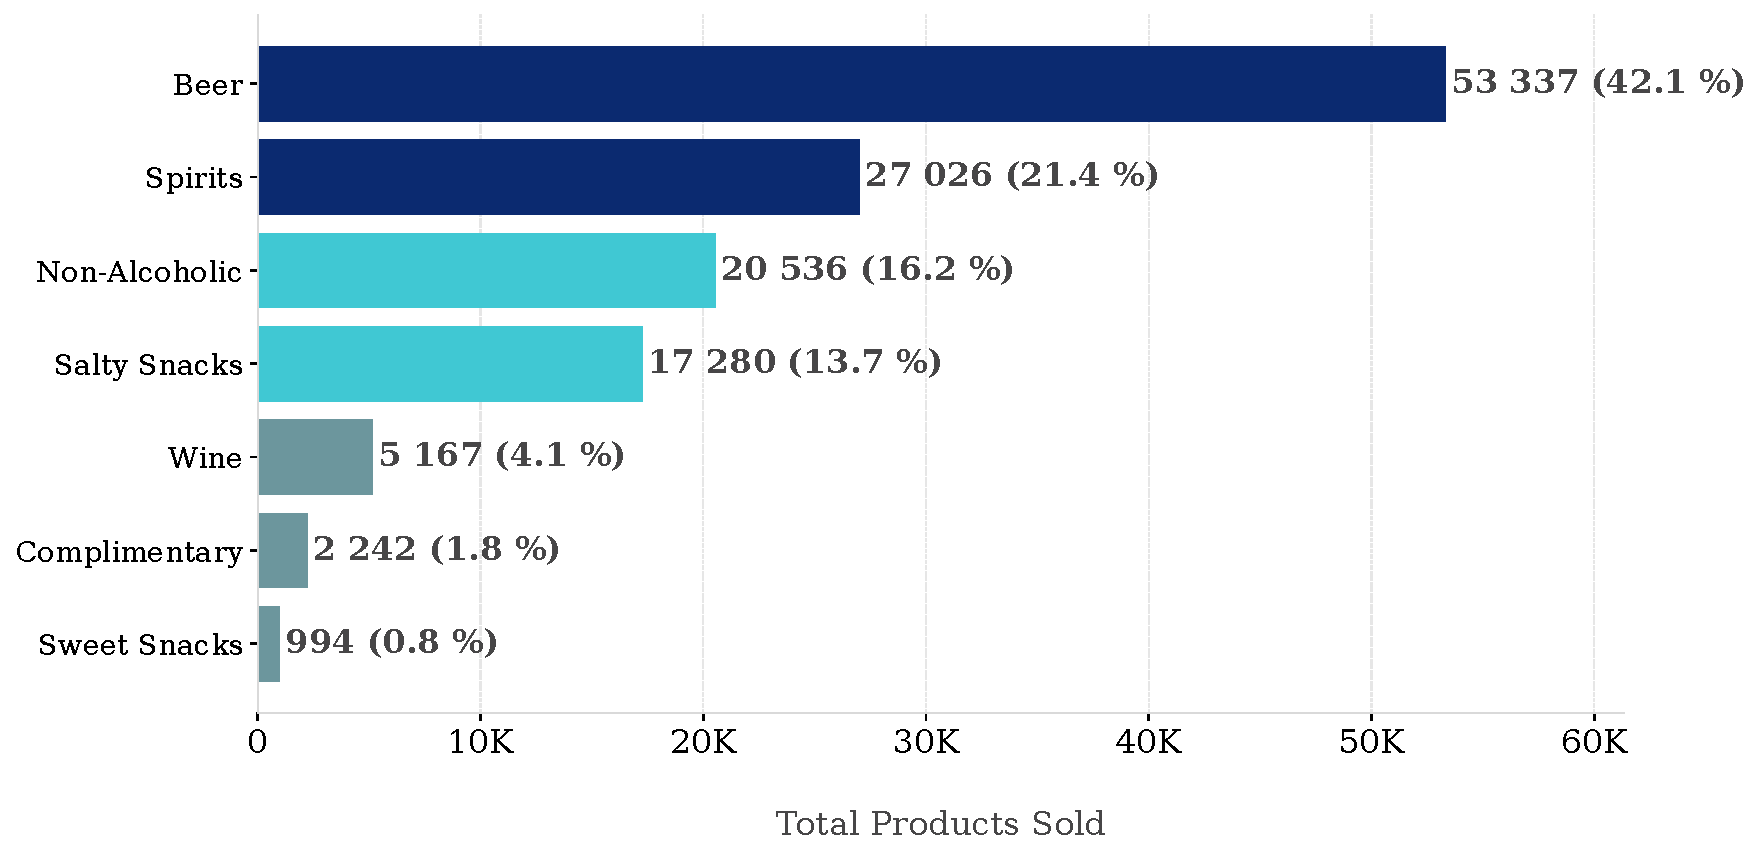
\includegraphics[width=\textwidth]{\ChartsDir/rq11-best-product-category}
	\caption{\rqshorttext{performance-best-products} Best Products by Category}
	\label{fig:best-product-category}
	\source
\end{figure}

This chart now confirms the prediction about the beer beverages, as the \textbf{Beer} (Pivo) category was the most sold during the event with a little more than~\bfmtnum{40000}~orders processed.

\begin{keytakeaways}
	\begin{itemize}
		\item The best product was a returnable cup followed by beer beverages.
		\item Prediction about the beer beverages was confirmed, as the \textbf{Beer} (Pivo) category was the most sold during the event.
	\end{itemize}
\end{keytakeaways}

This last analysis provided insights into the best products, which confirmed the previous predictions and will now serve as a basis for the next section, where the beverage consumption will be analyzed.

%%% Performance / Summary
%%% --------------------------------------------------------------

\subsection{Summary}
\label{subsec:analysis-performance-indicators-summary}

Thanks to this section, the performance indicators of the event were analyzed, and the key metrics were identified.
The results analyzed the transactional processing performance, identified several peak points during the event, and provided insights into the best sale points, top-up points, vendors, and products.
Providing a better understanding of the event's performance and giving more context for the next analysis dealing with the beverage consumption.

%%% Section: Beverage Consumption Analysis
%%% --------------------------------------------------------------


\section{Beverage Consumption Analysis}
\label{sec:analysis-beverage-consumption}

% TODO: rephrase, too repetitive
This section will provide a detailed analysis of beverage consumption, which was previously established as the most significant aspect of the event.

% TODO: rephrase, too repetitive
It should offer insights into overall consumption, detailed information on returnable cups, the most often drank beverages, and the leading beverage brands, addressing the previously established inquiries.

This section will address the next six research questions, after a minor logical reorganization into three groups:
\begin{enumerate}
	\item \fullref{subsec:analysis-beverage-returnable-cups}
	\item \fullref{subsec:analysis-beverage-total-consumption}
	\item and~\fullref{subsec:analysis-beverage-popular-brands}.
\end{enumerate}

%%% Beverage / Returnable Cups Analysis
%%% --------------------------------------------------------------

\subsection{Returnable Cups Analysis}
\label{subsec:analysis-beverage-returnable-cups}

Due to the little alteration of the local database and the previously referenced data in~\autoref{subsec:data-methodology-local-database-modifications}, it became possible to monitor the returnable cups and their associated transactions.

This capability, previously absent, should enhance comprehension of product sales and the utilization of returnable cups.

\makerqbox{beverage-returnable-cups}

To figure out the results, it was essential to analyze the actual contents of the transactions rather than merely identifying transactions including returnable cups,
as a single transaction may encompass many products and hence multiple returnable cups.
The organizer sold the cups for a price of ~\fmtczk{70} with a ~\fmtnum{21}\% VAT.\

Upon calculating the total number of issued and returned cups, the results depicted in~\autoref{fig:returnable-cups}~below illustrate the distribution of returnable cups throughout the event.

\begin{figure}[H]
	\centering
	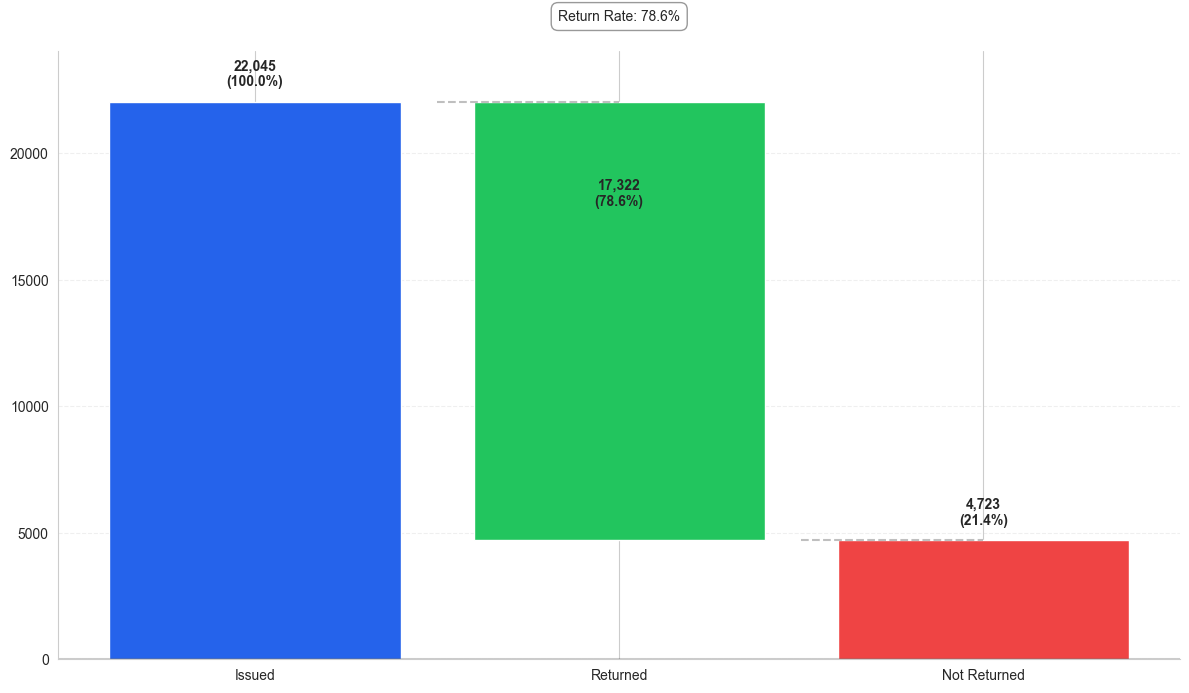
\includegraphics[width=\textwidth]{\ChartsDir/rq13-returnable-cups}
	\caption{\rqshorttext{beverage-returnable-cups} Returnable Cups}
	\label{fig:returnable-cups}
	\source
\end{figure}

The data indicate that a total of~\bfmtnum{20045}~cups was distributed during the event, with only~\bfmtnum{17322}~cups returned, yielding a return rate of~\bfmtnump[2]{78.60}\%.

This, however, does not imply that the remaining~\bfmtnum{4723}~cups were lost or regarded as a loss, as the cups were purchased.
Most unreturned cups can be presumed to have been retained as souvenirs.

\begin{keytakeaways}
	\begin{itemize}
		\item The total of~\bfmtnum{20045}~cups were issued during the festival.
		\item Only~\bfmtnum{17322}~cups returned resulted in a~\bfmtnump[2]{78.60}\%~return rate.
	\end{itemize}
\end{keytakeaways}

%%% Beverage / Total Consumption Analysis
%%% --------------------------------------------------------------

\subsection{Total Consumption Analysis}
\label{subsec:analysis-beverage-total-consumption}

This focuses on the overall beverage consumption during the event.
Again, thanks to local database modifications, it was possible to track the beverage consumption easily, as each product now had a volume attribute in milliliters.

\makerqbox{beverage-total-consumption}

To find the results was quite straightforward, as it only required summing up the volumes of all sold products.

However, to present the results, it was convenient to group the products into categories and show the total consumption of each category and thus answering also the next question~\rqshort{beverage-popular-category}.

\makerqbox{beverage-popular-category}

These results are shown in the~\autoref{tab:beverage-total-consumption} below and show a total of~\bfmtnum{29342}~liters of beverages consumed during the event with the beer category being the most consumed.

\begin{table}[H]
	\centering
	\begin{tabularx}{\textwidth}{|>{\columncolor{unicorn_blue!5}}X|>{\columncolor{unicorn_blue!5}}r|>{\columncolor{unicorn_blue!5}}r|}
		\hline
		\rowcolor{unicorn_blue}
		\textbf{\color{white}Beverage Category}
		& \textbf{\color{white}Volume}
		& \textbf{\color{white}Ratio}
		\\
		\hline
		\hline
		\colorindicator{1}Beer                    & \fmtnum{19797}~l  & \fmtnump[2]{67.46}~\% \\
		\colorindicator{2}Non-alcoholic           & \fmtnum{6987}~l   & \fmtnump[2]{23.81}~\% \\
		\colorindicator{3}Spirits / other alcohol & \fmtnum{1992}~l   & \fmtnump[2]{6.78}~\%  \\
		\colorindicator{4}Wine                    & \fmtnum{575}~l    & \fmtnump[2]{1.95}~\%  \\
		\hline
		\textbf{Total volume}                     & \bfmtnum{29342}~l & \fmtnum{100}~\%       \\
		\hline
	\end{tabularx}
	\caption{\rqshorttext{beverage-total-consumption} Total Beverage Consumption}
	\label{tab:beverage-total-consumption}
\end{table}

These results serve as a basis for the next questions, which focuses on the most consumed beverage brands rather than product categories.

\begin{keytakeaways}
	\begin{itemize}
		\item The total of~\bfmtnum{29342}~liters of beverages were consumed during the event.
		\item The beer category was the most consumed with~\bfmtnum{19797}~liters consumed.
	\end{itemize}
\end{keytakeaways}

%%% Beverage / Popular Brands Analysis
%%% --------------------------------------------------------------

\subsection{Popular Brands Analysis}
\label{subsec:analysis-beverage-popular-brands}

This section explores beverage preferences, concentrating on the most popular brands within the leading categories:
\begin{itemize}
	\item \fullref{subsubsec:analysis-beverage-popular-beer},
	\item \fullref{subsubsec:analysis-beverage-popular-non-alcoholic},
	\item and~\fullref{subsubsec:analysis-beverage-popular-alcoholic}.
\end{itemize}

Answering these issues required the identification and categorization of all beverage products, followed by the computation of their overall consumption.
However, this was not entirely easy, as the products were not uniformly labeled.
This indicated that beers labeled as~\enquote{Radegast 10} and~\enquote{Radegast 12} were not categorized together, resulting in biased outcomes.

To address this issue, the products ought to be categorized by their brand rather than by their name.
This methodology seemed logical; nevertheless, the data lacked brand information, containing simply the product name.

A systematic approach would be to extend the database with brands and back-fill the products with a link to the brand.
This would require a significant amount of work and time, which was not available at the time of this analysis.

A more straightforward and manual method was used, wherein the product's~\enquote{brand} was identified by extracting the essential parts of the product name, eliminating redundant elements such as volume, beer grade, or other details.
This helped produce better results, however, still lack complete accuracy.

%%% Beverage / Popular Brands Analysis / Beer Brands Analysis
%%% --------------------------------------------------------------

\subsubsection{Beer Brands Analysis}
\label{subsubsec:analysis-beverage-popular-beer}
Starting with the most consumed and most popular category – beer.

\makerqbox{beverage-top-beer}

The results in~\autoref{fig:beverage-top-beer} below illustrate the distribution of the most frequently consumed beer brands during the event.

\begin{figure}[H]
	\centering
	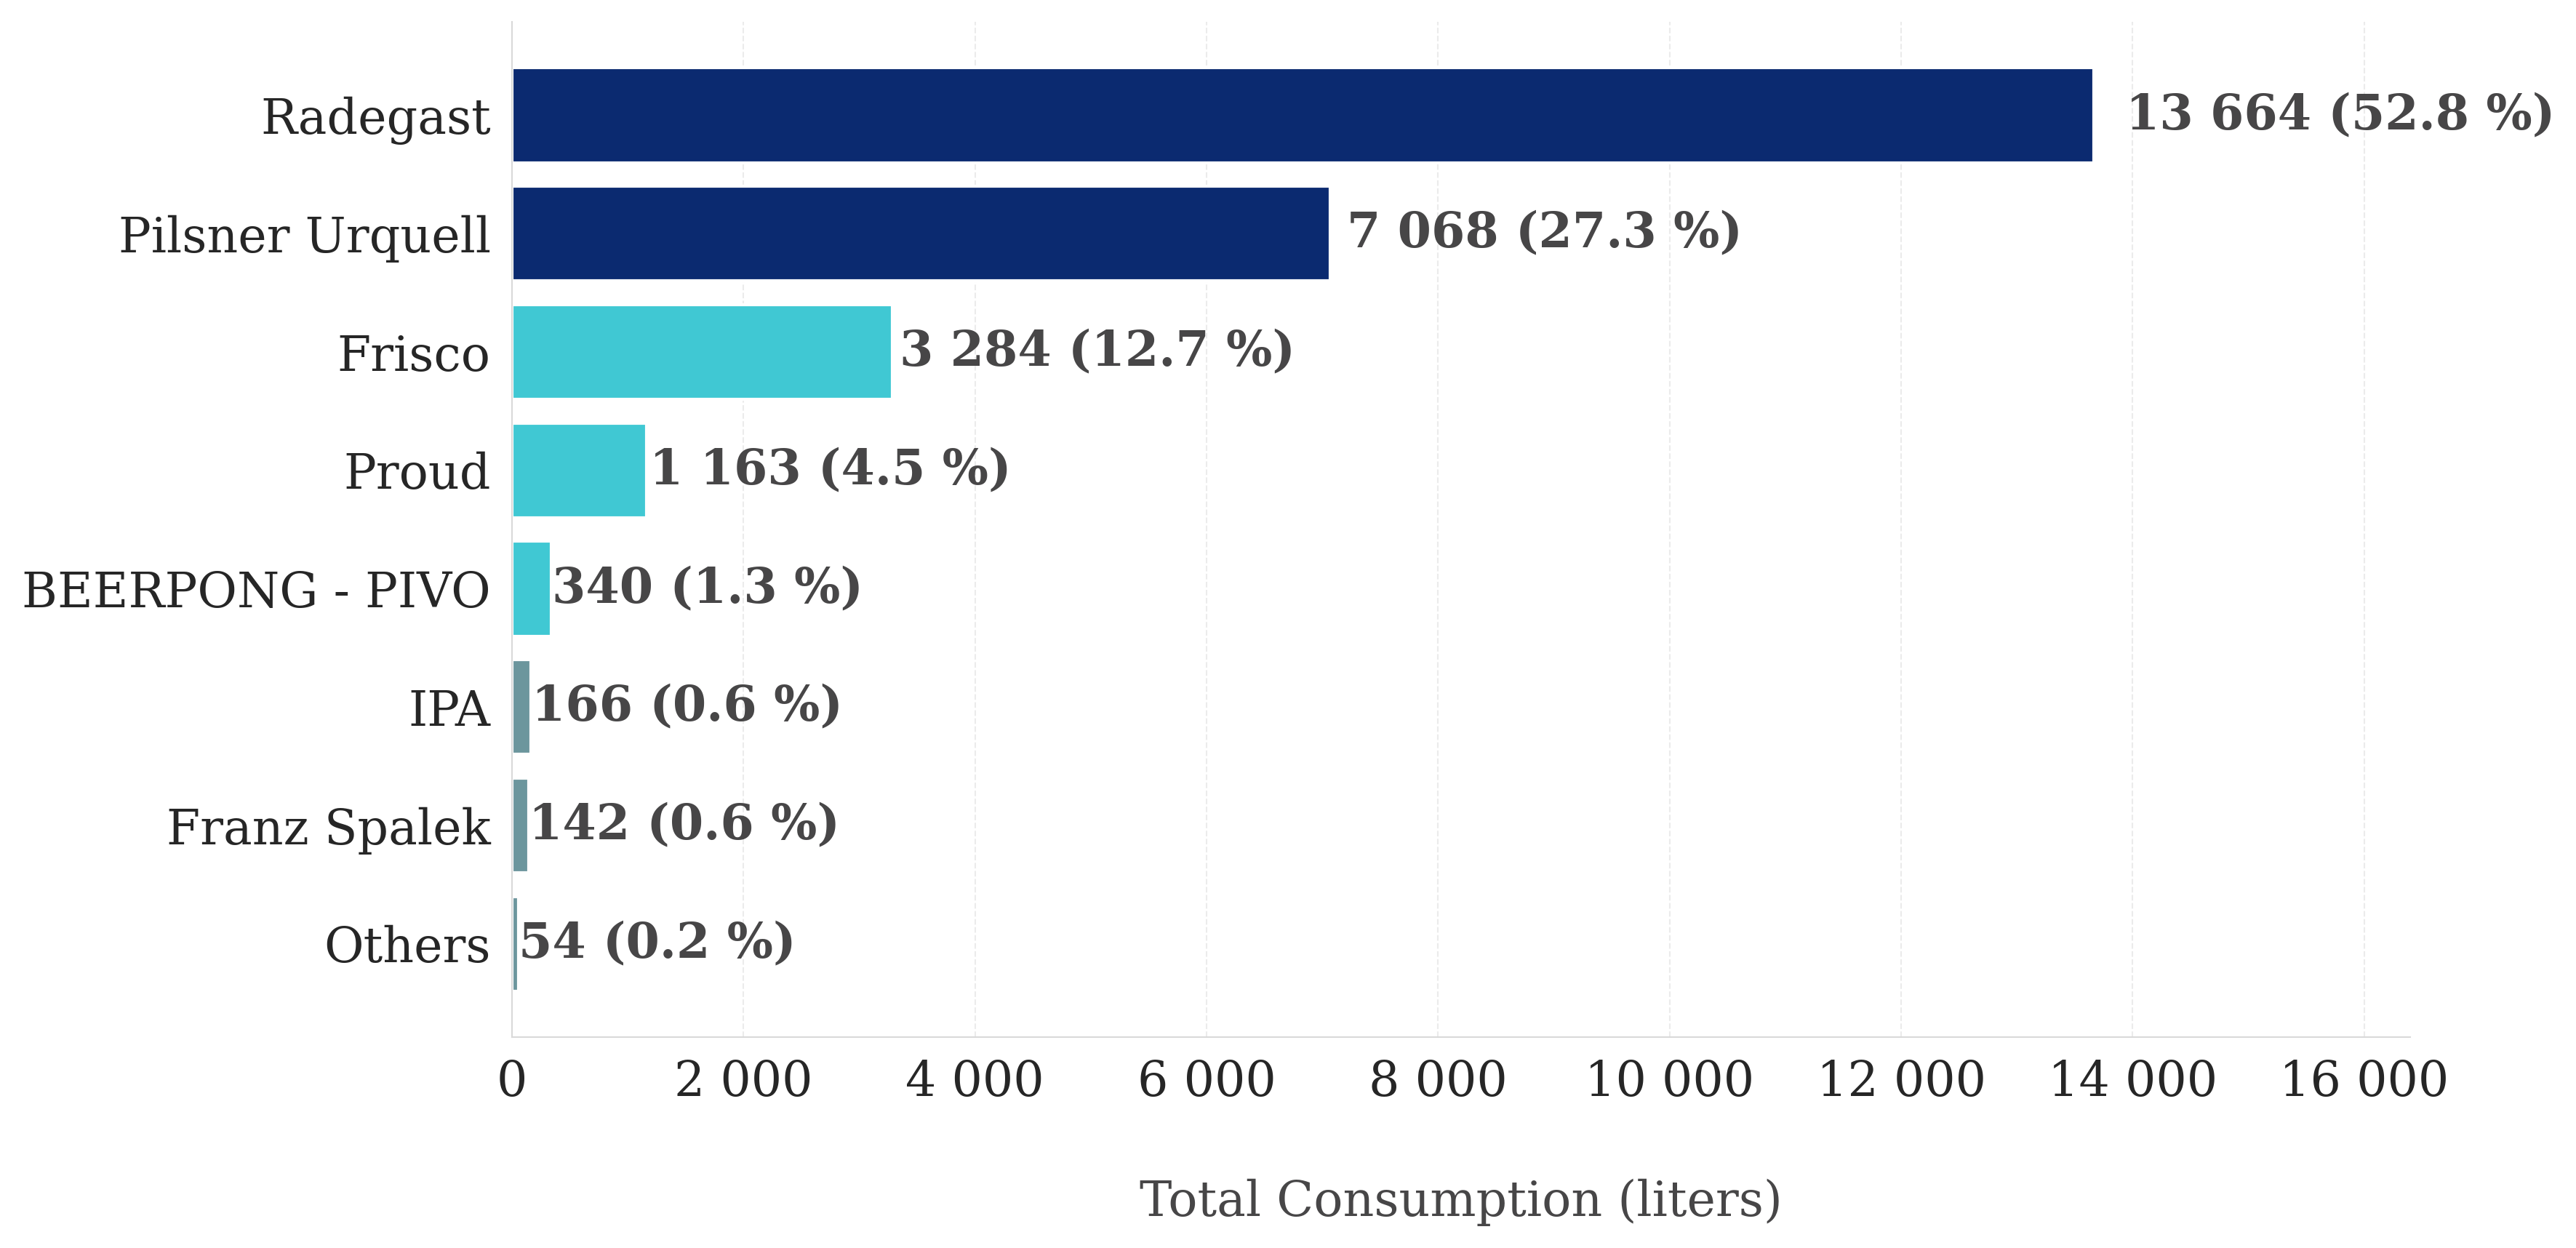
\includegraphics[width=\textwidth]{\ChartsDir/rq15-top-beer-brands}
	\caption{\rqshorttext{beverage-top-beer} Most Consumed Beer Brands}
	\label{fig:beverage-top-beer}
	\source
\end{figure}

This distribution indicates that the most consumed beer brand was \textbf{Radegast}, with a total consumption of~\bfmtnum{10366}~liters and~\bfmtnum{27329} units sold.

The second was \textbf{Pilsner Urquell}, which had half the consumption of \textbf{Radegast}, followed by the \textbf{Frisco} and \textbf{Proud} brands.
A complete list of all ten brands from the festival is shown in the~\autoref{tab:beverage-top-beer}~below.

\begin{table}[htbp]
	\centering
	\small
	\begin{tabularx}{\textwidth}{
		|>{\columncolor{unicorn_blue!5}\centering\arraybackslash}p{1cm}
		|>{\columncolor{unicorn_blue!5}\raggedright\arraybackslash}X
		|>{\columncolor{unicorn_blue!5}\raggedleft\arraybackslash}p{4cm}
		|>{\columncolor{unicorn_blue!5}\raggedleft\arraybackslash}p{2.5cm}|}
		\hline
		\rowcolor{unicorn_blue}
		\textbf{}
		& \textbf{\color{white}Beer brand}
		& \textbf{\color{white}Total consumption}
		& \textbf{\color{white}Units sold}
		\\\hline\hline
% rows
		\csvreader[
			head to column names,
			late after line={\\\hline},
		]{\DataDir/rq15-top-beer-brands.csv}{
			subcategory=\colbrand,
			total_consumption_ml=\colconsumption,
			transaction_count=\coltrxcount,
			total_sold=\colunits
		}{
			\the\numexpr\thecsvinputline-1
			& \colbrand
			& \num[group-separator={,}]{\colconsumption}~l
			& \num[group-separator={,}]{\colunits}
		}
		\hline
		\noalign{\vspace{1mm}}
		\hline
		\rowcolor{unicorn_blue!20}
		\textbf{}
		& \textbf{Total}
		& {\bfmtnum{19793}}~l
		& {\bfmtnum{53990}}
		\\\hline
	\end{tabularx}
	\caption{\rqshorttext{beverage-top-beer} Most Consumed Beer Brands}
	\label{tab:beverage-top-beer}
\end{table}

The data demonstrate a strong preference for Radegast beer among festival attendees.
The price may have influenced this, as the Radegast was generally slightly less expensive than, for instance, the Pilsner Urquell.

\begin{keytakeaways}
	\begin{itemize}
		\item The most consumed beer brand was \textbf{Radegast} with a total of~\bfmtnum{10366}~liters consumed.
		\item The second most consumed beer brand was the \textbf{Pilsner Urquell} with half the consumption of the Radegast.
	\end{itemize}
\end{keytakeaways}

%%% Beverage / Popular Brands Analysis / Non-alcoholic Brands Analysis
%%% --------------------------------------------------------------

\subsubsection{Non-alcoholic Brands Analysis}
\label{subsubsec:analysis-beverage-popular-non-alcoholic}

This next section is bound to the non-alcoholic beverages, which were the second most consumed category.

\makerqbox{beverage-top-non-alcoholic}

Aggregated similarly as in the previous analysis, the results in the~\autoref{tab:beverage-top-non-alcoholic}~below show the distribution of the most consumed non-alcoholic brands during the event.

\begin{table}[htbp]
	\centering
	\small
	\begin{tabularx}{\textwidth}{
		|>{\columncolor{unicorn_blue!5}\centering\arraybackslash}p{1cm}
		|>{\columncolor{unicorn_blue!5}\raggedright\arraybackslash}X
		|>{\columncolor{unicorn_blue!5}\raggedleft\arraybackslash}p{4cm}
		|>{\columncolor{unicorn_blue!5}\raggedleft\arraybackslash}p{2.5cm}|}
		\hline
		\rowcolor{unicorn_blue}
		\textbf{}
		& \textbf{\color{white}Non-alcoholic brand}
		& \textbf{\color{white}Total consumption}
		& \textbf{\color{white}Units sold}
		\\\hline\hline
% rows
		\csvreader[
			head to column names,
			late after line={\\\hline},
		]{\DataDir/rq17-top-non-alco-brands.csv}{
			subcategory=\colbrand,
			total_consumption_ml=\colconsumption,
			transaction_count=\coltrxcount,
			total_sold=\colunits
		}{
			\the\numexpr\thecsvinputline-1
			& \colbrand
			& \num[group-separator={,}]{\colconsumption}~l
			& \num[group-separator={,}]{\colunits}
		}
		\hline
		\noalign{\vspace{1mm}}
		\hline
		\rowcolor{unicorn_blue!20}
		\textbf{}
		& \textbf{Total}
		& {\bfmtnum{6971}}~l
		& {\bfmtnum{20487}}
		\\\hline
	\end{tabularx}
	\caption{\rqshorttext{beverage-top-non-alcoholic} Most Consumed Non-alcoholic Brands}
	\label{tab:beverage-top-non-alcoholic}
\end{table}

The results indicate a close rivalry between the \textbf{Birell} and \textbf{ZON Lemonade} brands, with Birell emerging as the most consumed non-alcoholic beverage at the event.
A total of~\bfmtnum{6971}~liters drank and~\bfmtnum{20487}~units sold established it as the most popular non-alcoholic beverage, commanding a~\bfmtnump[2]{31.35}\%~share of the total consumption.

\begin{keytakeaways}
	\begin{itemize}
		\item The most consumed non-alcoholic brand was \textbf{Birell} with a total of~\bfmtnum{2186}~liters consumed.
		\item The second most consumed non-alcoholic brand was the \textbf{ZON Lemonade}.
	\end{itemize}
\end{keytakeaways}

%%% Beverage / Popular Brands Analysis / Alcoholic Brands Analysis
%%% --------------------------------------------------------------

\subsubsection{Alcoholic Brands Analysis}
\label{subsubsec:analysis-beverage-popular-alcoholic}

The last part of this section focuses on other alcoholic beverages, such as spirits, shots, cocktails, and other alcoholic beverages.

\makerqbox{beverage-top-alcoholic}

This analysis consisted of a total of 23 different brands consisting mostly of spirits and shots.
Results presented in this section may be more biased than the previous ones, as the brand determination was more difficult due to the lack of consistent labeling.
Moreover, previously it was necessary to classify the products with the volume information, which is not so straightforward for shots and spirits.

The results in the~\autoref{tab:beverage-top-alcoholic}~indicate that the most consumed alcoholic brand was the \textbf{Beefeater} with a total of~\bfmtnum{966}~liters consumed and~\bfmtnum{4628}~units sold.
However, the second most consumed brand was \textbf{Absolut Vodka} with only \bfmtnum{335}~liters consumed, but with a much higher units sold count of~\bfmtnum{9177}.

\begin{table}[htbp]
	\centering
	\small
	\begin{tabularx}{\textwidth}{
		|>{\columncolor{unicorn_blue!5}\centering\arraybackslash}p{1cm}
		|>{\columncolor{unicorn_blue!5}\raggedright\arraybackslash}X
		|>{\columncolor{unicorn_blue!5}\raggedleft\arraybackslash}p{4cm}
		|>{\columncolor{unicorn_blue!5}\raggedleft\arraybackslash}p{2.5cm}|}
		\hline
		\rowcolor{unicorn_blue}
		\textbf{}
		& \textbf{\color{white}Alcoholic brand}
		& \textbf{\color{white}Total consumption}
		& \textbf{\color{white}Units sold}
		\\\hline\hline
% rows
		\csvreader[
			head to column names,
			late after line={\\\hline},
		]{\DataDir/rq16-top-alco-brands.csv}{
			subcategory=\colbrand,
			total_consumption_ml=\colconsumption,
			transaction_count=\coltrxcount,
			total_sold=\colunits
		}{
			\the\numexpr\thecsvinputline-1
			& \colbrand
			& \num[group-separator={,}]{\colconsumption}~l
			& \num[group-separator={,}]{\colunits}
		}
		\hline
		\noalign{\vspace{1mm}}
		\hline
		\rowcolor{unicorn_blue!20}
		\textbf{}
		& \textbf{Total}
		& {\bfmtnum{1980}}~l
		& {\bfmtnum{26964}}
		\\\hline
	\end{tabularx}
	\caption{\rqshorttext{beverage-top-alcoholic} Most Consumed Alcoholic Brands}
	\label{tab:beverage-top-alcoholic}
\end{table}

\begin{keytakeaways}
	\begin{itemize}
		\item The most consumed alcoholic brand was the \textbf{Beefeater} with a total of~\bfmtnum{966}~liters consumed.
		\item The second most consumed alcoholic brand was the \textbf{Absolut Vodka} with a total of~\bfmtnum{335}~liters consumed.
	\end{itemize}
\end{keytakeaways}

%%% Beverage / Summary
%%% --------------------------------------------------------------

\subsection{Summary}
\label{subsec:analysis-beverage-consumption-summary}

Insights into beverage consumption, covered in this section, should provide a better understanding of the overall preferences and total consumptions during the festival.
As this data was not previously available, it was a valuable addition to the analysis and will play a significant role when presenting the results to the festival organizers.

The results showed the total consumption of all beverages, the insightful view on returnable cups usage, and the most consumed beverage brands in the most popular categories.

With the data available, there are still many more questions that could be answered, particularly in combination with customer data.
However, clear bounds were set for this analysis to answer the most important questions asked by the festival organizers.

%%% Section: Customer Analysis
%%% --------------------------------------------------------------


\section{Customer Analysis}
\label{sec:analysis-customers}

This section will focus on customer analysis, which should provide interesting insights into festival attendees' behavior and segmentation.

Because the organizers lacked deeper insights into festival attendees, this analysis should contribute significantly to a better understanding of the event.

The analysis addresses the remaining research questions, which have been reorganized into four logical groups to improve the narrative flow:
\begin{enumerate}
	\item \fullref{subsec:analysis-customer-event-attendance-timeline},
	\item \fullref{subsec:analysis-customer-segmentation},
	\item \fullref{subsec:analysis-customer-payment-behavior},
	\item and~\fullref{subsec:analysis-customer-purchase-pattern}.
\end{enumerate}

%%% Customer / Event Attendance and Timeline Analysis
%%% --------------------------------------------------------------

\subsection{Event Attendance and Timeline Analysis}
\label{subsec:analysis-customer-event-attendance-timeline}

This section should provide information about attendees' initial behavior, total attendance throughout the festival, and subsequent top-up behavior.

%%% Customer / Event Attendance and Timeline Analysis / Total Attendance and Daily Activity
%%% --------------------------------------------------------------

\subsubsection{Total Attendance and Daily Activity}
\label{subsubsec:analysis-total-attendance}

% FIXME
\makerqbox{customers-total-attendance}

The analysis shows that the festival attracted a total of~\bfmtnum{10009}~unique customers over the three-day duration.
However, the daily attendance figures show interesting patterns in how these customers were distributed throughout the festival days.

Looking at the daily active customers:
\begin{itemize}
	\item Day 1 (Thursday):~\bfmtnum{6214}~active customers
	\item Day 2 (Friday):~\bfmtnum{5832}~active customers
	\item Day 3 (Saturday):~\bfmtnum{8066}~active customers
\end{itemize}

These numbers indicate that many customers attended multiple days of the festival, as the sum of daily attendees (\bfmtnum{20112}) is significantly higher than the unique customer count.
This was expected, as the festival was designed to attract visitors for multiple days.

The attendance peaked on the final day of the festival, with Day 2 showing slightly lower attendance than the opening day.
The significant increase in attendance on Day 3 suggests that the festival successfully attracted weekend visitors.

\begin{keytakeaways}
	\begin{itemize}
		\item Total unique customers over the three days:~\bfmtnum{10009}.
		\item The highest attendance was on Day 3 (Saturday) with~\bfmtnum{8066}~active customers.
		\item The festival maintained consistent attendance on weekdays (Days 1–2).
		\item Significant increase in attendance (38\% higher than Day 2) for the weekend (Day 3).
	\end{itemize}
\end{keytakeaways}

%%% Customer / Event Attendance and Timeline Analysis / Visitor Arrival Patterns
%%% --------------------------------------------------------------

\subsubsection{Visitor Arrival Patterns}
\label{subsubsec:analysis-visitor-patterns}

\makerqbox{customers-new-visitors}

The analysis of visitor arrival patterns reveals distinct peak periods across the three festival days, with significant variations in the rate of new visitor registrations throughout each day.

\begin{figure}[H]
	\centering
	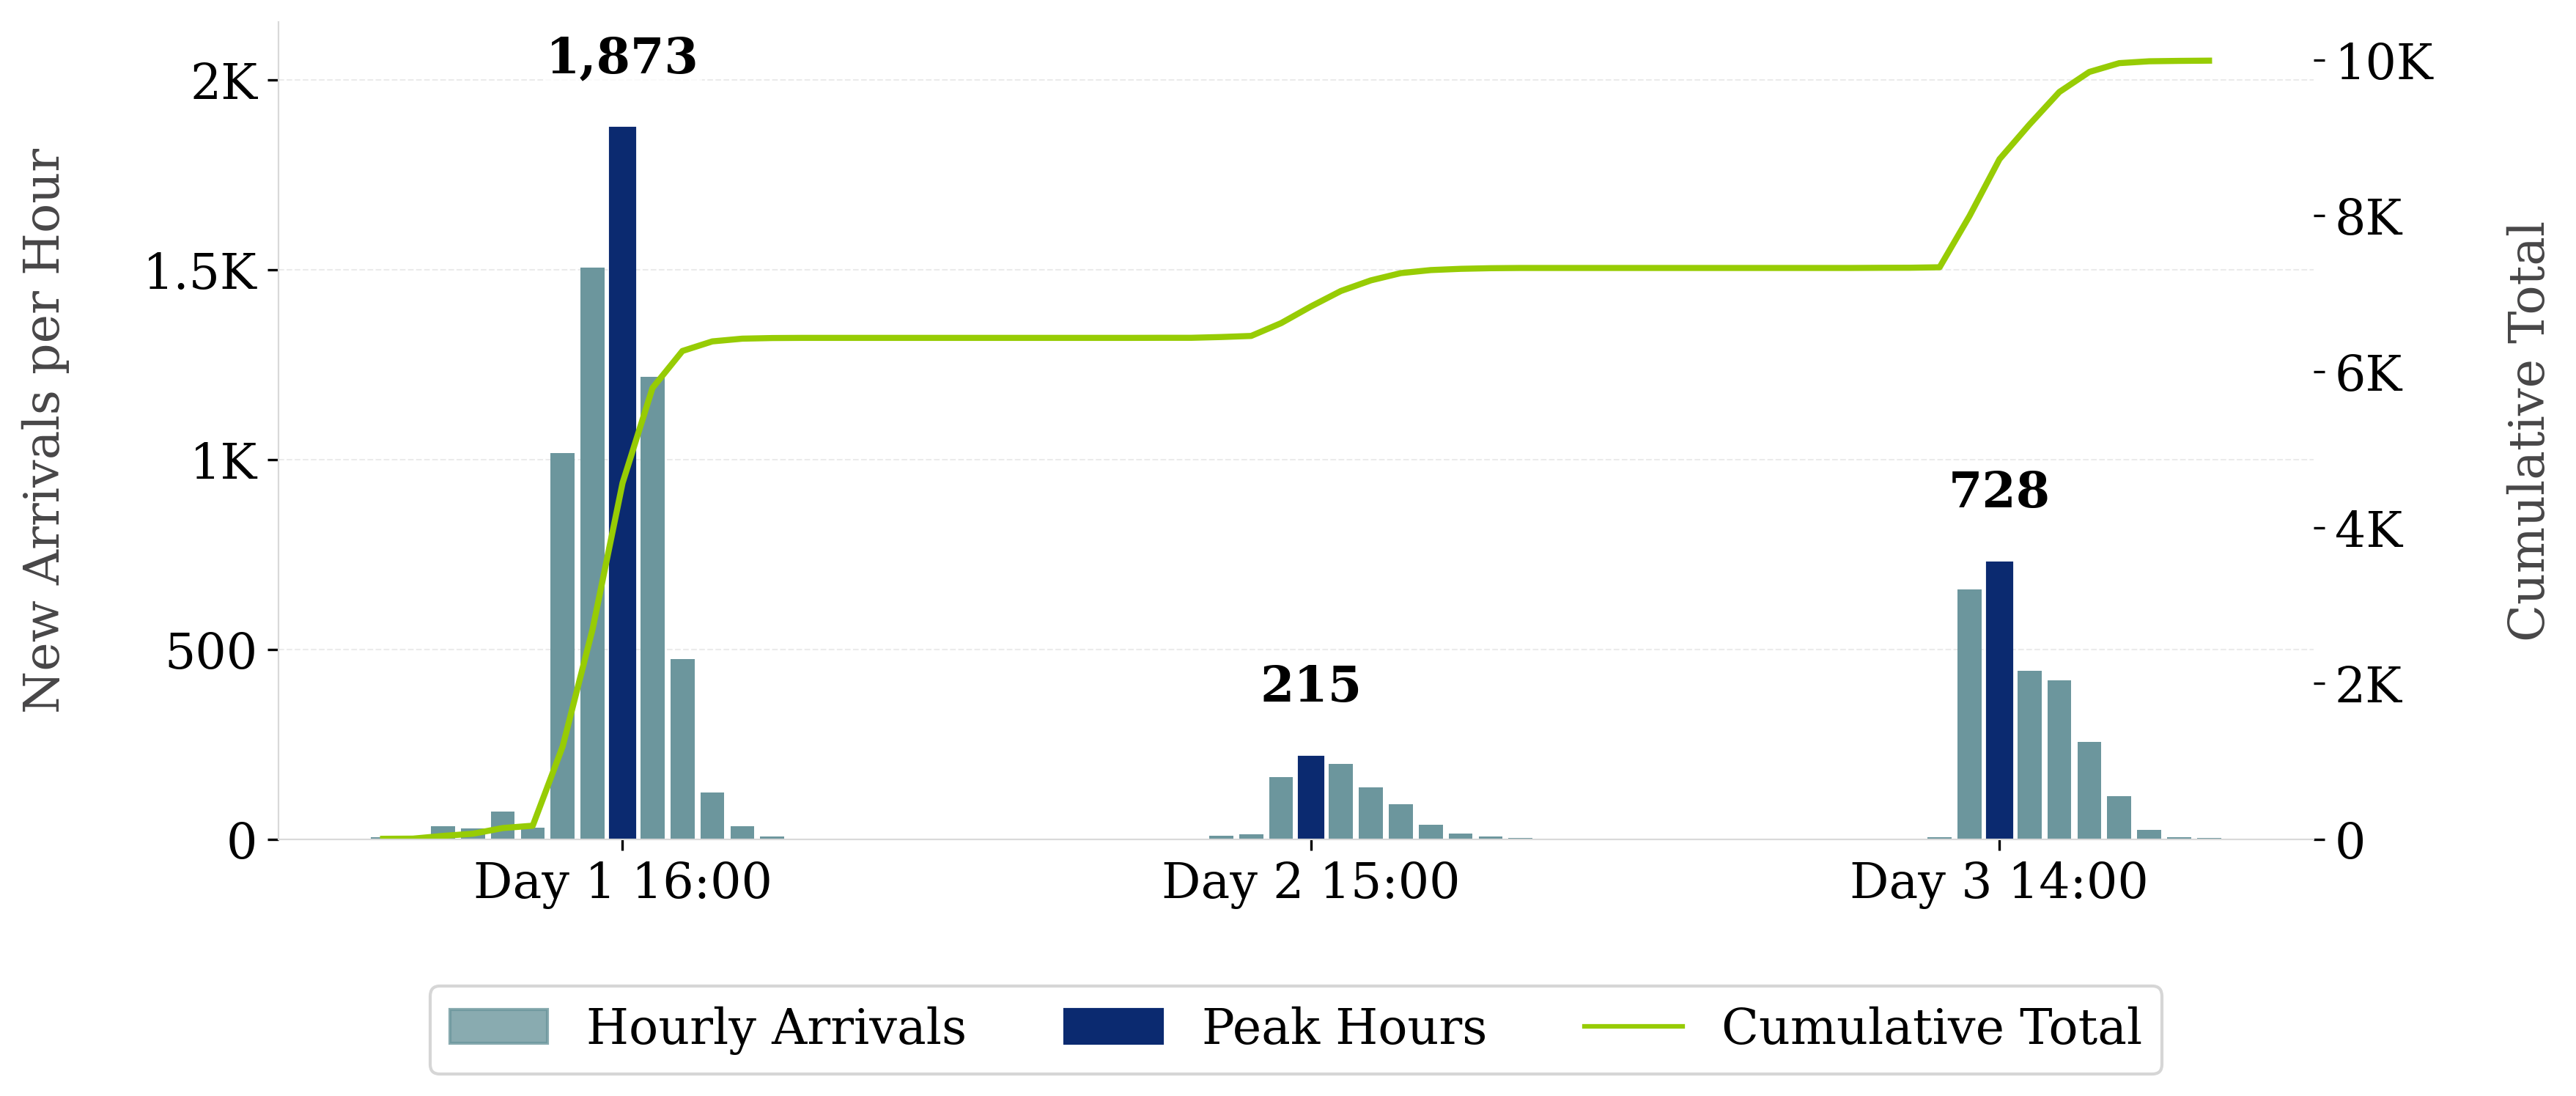
\includegraphics[width=\textwidth]{\ChartsDir/rq24-arrival-patterns}
	\caption{\rqshorttext{customers-new-visitors} Visitor Arrival Patterns}
	\label{fig:visitor-arrival-patterns}
	\source
\end{figure}

The data reveals three distinct patterns across the festival days:

\begin{itemize}
	\item \textbf{Day 1 (Thursday)}: A rapid peak of approximately~\bfmtnum{1873}~new visitors was observed during the 16:00 hour, which was the time of the highest arrival activity.
	The day showed a clear pattern of increasing arrivals from 14:00 to 16:00, followed by a gradual decline resulting in a total of~\bfmtnum{6433}~new visitors.
	\item \textbf{Day 2 (Friday)}: A modest peak of~\bfmtnum{215}~visitors at 15:00, but significantly lower new arrivals than on Day 1.
	This decrease in the number of new arrivals was expected, as a significant number of visitors had already completed the registration process on Day 1.
	\item \textbf{Day 3 (Saturday)}: The weekend attendees' influx was clear in the resurgence of new arrivals, which reached a peak of~\bfmtnum{728}~new visitors at 14:00.
\end{itemize}

The data indicates that the majority of visitor arrivals occurred during the afternoon hours (14:00–17:00) on all days.
Minimal new arrivals were consistently observed during the early morning hours (before 10:00) and late evening hours (after 20:00).

\begin{keytakeaways}
	\begin{itemize}
		\item Highest single-hour registration peak:~\bfmtnum{1873}~visitors (Day 1, 16:00).
		\item The registration window that was most effective was from 14:00 to 17:00 on all days.
		\item Day 1 accounted for approximately~\bfmtnump[2]{64.39}\%~of total arrivals.
		\item Weekend (Day 3) saw renewed registration activity with peak of~\bfmtnum{728}~new visitors.
	\end{itemize}
\end{keytakeaways}

%%% Customer / Event Attendance and Timeline Analysis / Top-Up Peaks
%%% --------------------------------------------------------------

\subsubsection{Time to First Transaction}
\label{subsubsec:analysis-first-transaction}

\makerqbox{customers-visitor-time}

The analysis reveals significant variations in how quickly different types of visitors made their first transaction after arrival.
Overall, the average time to the first transaction was~\bfmtnum{79.55}~minutes.
However, this number alone is misleading, as evidenced by the much lower median of~\bfmtnum{7}~minutes and mode of~\bfmtnum{3}~minutes.

\begin{table}[H]
	\centering
	\small
	\begin{tabularx}{\textwidth}{
		|>{\columncolor{unicorn_blue!5}\centering\arraybackslash}l
		|>{\columncolor{unicorn_blue!5}\raggedleft\arraybackslash}X
		|>{\columncolor{unicorn_blue!5}\raggedleft\arraybackslash}X
		|>{\columncolor{unicorn_blue!5}\raggedleft\arraybackslash}X
		|>{\columncolor{unicorn_blue!5}\raggedleft\arraybackslash}X|
	}
		\hline
		\rowcolor{unicorn_blue}
		\textbf{\color{white}Visitor Type}
		& \textbf{\color{white}Average}
		& \textbf{\color{white}Mode}
		& \textbf{\color{white}Median}
		& \textbf{\color{white}Max}
		\\
		\hline
		\colorindicator{1}Guest
		& \textbf{2}~h~\textbf{21}~min
		& \bfmtnum{0}~min
		& \bfmtnum{10}~min
		& \textbf{52}~h~\textbf{56}~min
		\\
		\colorindicator{2}Regular
		& \bfmtnum{44.68}~min
		& \bfmtnum{0}~min
		& \bfmtnum{6}~min
		& \textbf{47}~h~\textbf{32}~min
		\\
		\colorindicator{3}Online
		& \bfmtnum{66.85}~min
		& \bfmtnum{3}~min
		& \bfmtnum{7}~min
		& \textbf{44}~h~\textbf{51}~min
		\\
		\colorindicator{4}Staff
		& \textbf{9}~h~\textbf{44}~min
		& \bfmtnum{7}~min
		& \textbf{3}~h~\textbf{54}~min
		& \textbf{58}~h~\textbf{12}~min
		\\
		\hline
		\rowcolor{unicorn_blue!20}
		\textbf{Overall}
		& \bfmtnum{79.55}~min
		& \bfmtnum{3}~min
		& \bfmtnum{7}~min
		& \textbf{58}~h~\textbf{12}~min
		\\
		\hline
	\end{tabularx}
	\caption{\rqshorttext{customers-visitor-time} Time to First Transaction}
	\label{tab:time-to-first-transaction}
	\source
\end{table}

Breaking down the analysis by visitor type\footnote{Visitor or rather, chip types are described in the~\fullref{tab:chip-types} table.}, reveals distinct patterns:
\begin{itemize}
	\item \textbf{Regular}: Quickest to transact, with an average of \bfmtnum{44.68} minutes and a median of only \bfmtnum{6} minutes
	\item \textbf{Online}: Similar efficiency with an average of \bfmtnum{66.85} minutes and a median of \bfmtnum{7} minutes
	\item \textbf{Guests}: Took longer, averaging \bfmtnum{140.59} minutes with a median of \bfmtnum{10} minutes
	\item \textbf{Staff}: Showed significantly different behavior, with an average of \bfmtnum{583.92} minutes and a median of \bfmtnum{234} minutes
\end{itemize}

The significant difference between average and median times across all categories suggests a right-skewed distribution, implying that while most visitors completed their first transaction quickly, others took much longer.
This was especially true for regular attendees, who would sometimes arrive early to check in and then return later to make their first purchase.

Staff members who were not there primarily to consume, on the other hand, exhibited a different behavior pattern, with their first transaction occurring later.
This was most likely due to their responsibilities at the event, which may have prevented them from making purchases during working hours.

\begin{keytakeaways}
	\begin{itemize}
		\item Most visitors (as indicated by the median) made their first transaction within~\bfmtnum{7}~minutes of arrival.
		\item Regular visitors were the most efficient, typically transacting within~\bfmtnum{6}~minutes.
		\item Staff members showed distinctly different behavior, likely due to their different role at the event.
		\item The large gap between mean and median times suggests some visitors waited significantly longer than others before their first transaction.
	\end{itemize}
\end{keytakeaways}

%%% Customer / Event Attendance and Timeline Analysis / Credit Top-up Patterns
%%% --------------------------------------------------------------

\subsubsection{Credit Top-up Patterns}
\label{subsubsec:analysis-credit-topup}

\makerqbox{customers-top-up-peaks}

The examination of credit top-up patterns reveals distinct peak periods and daily patterns throughout the event.
A total of~\bfmtnum{17233}~top-up transactions were processed, with activity varying significantly throughout the day.

\begin{figure}[H]
	\centering
	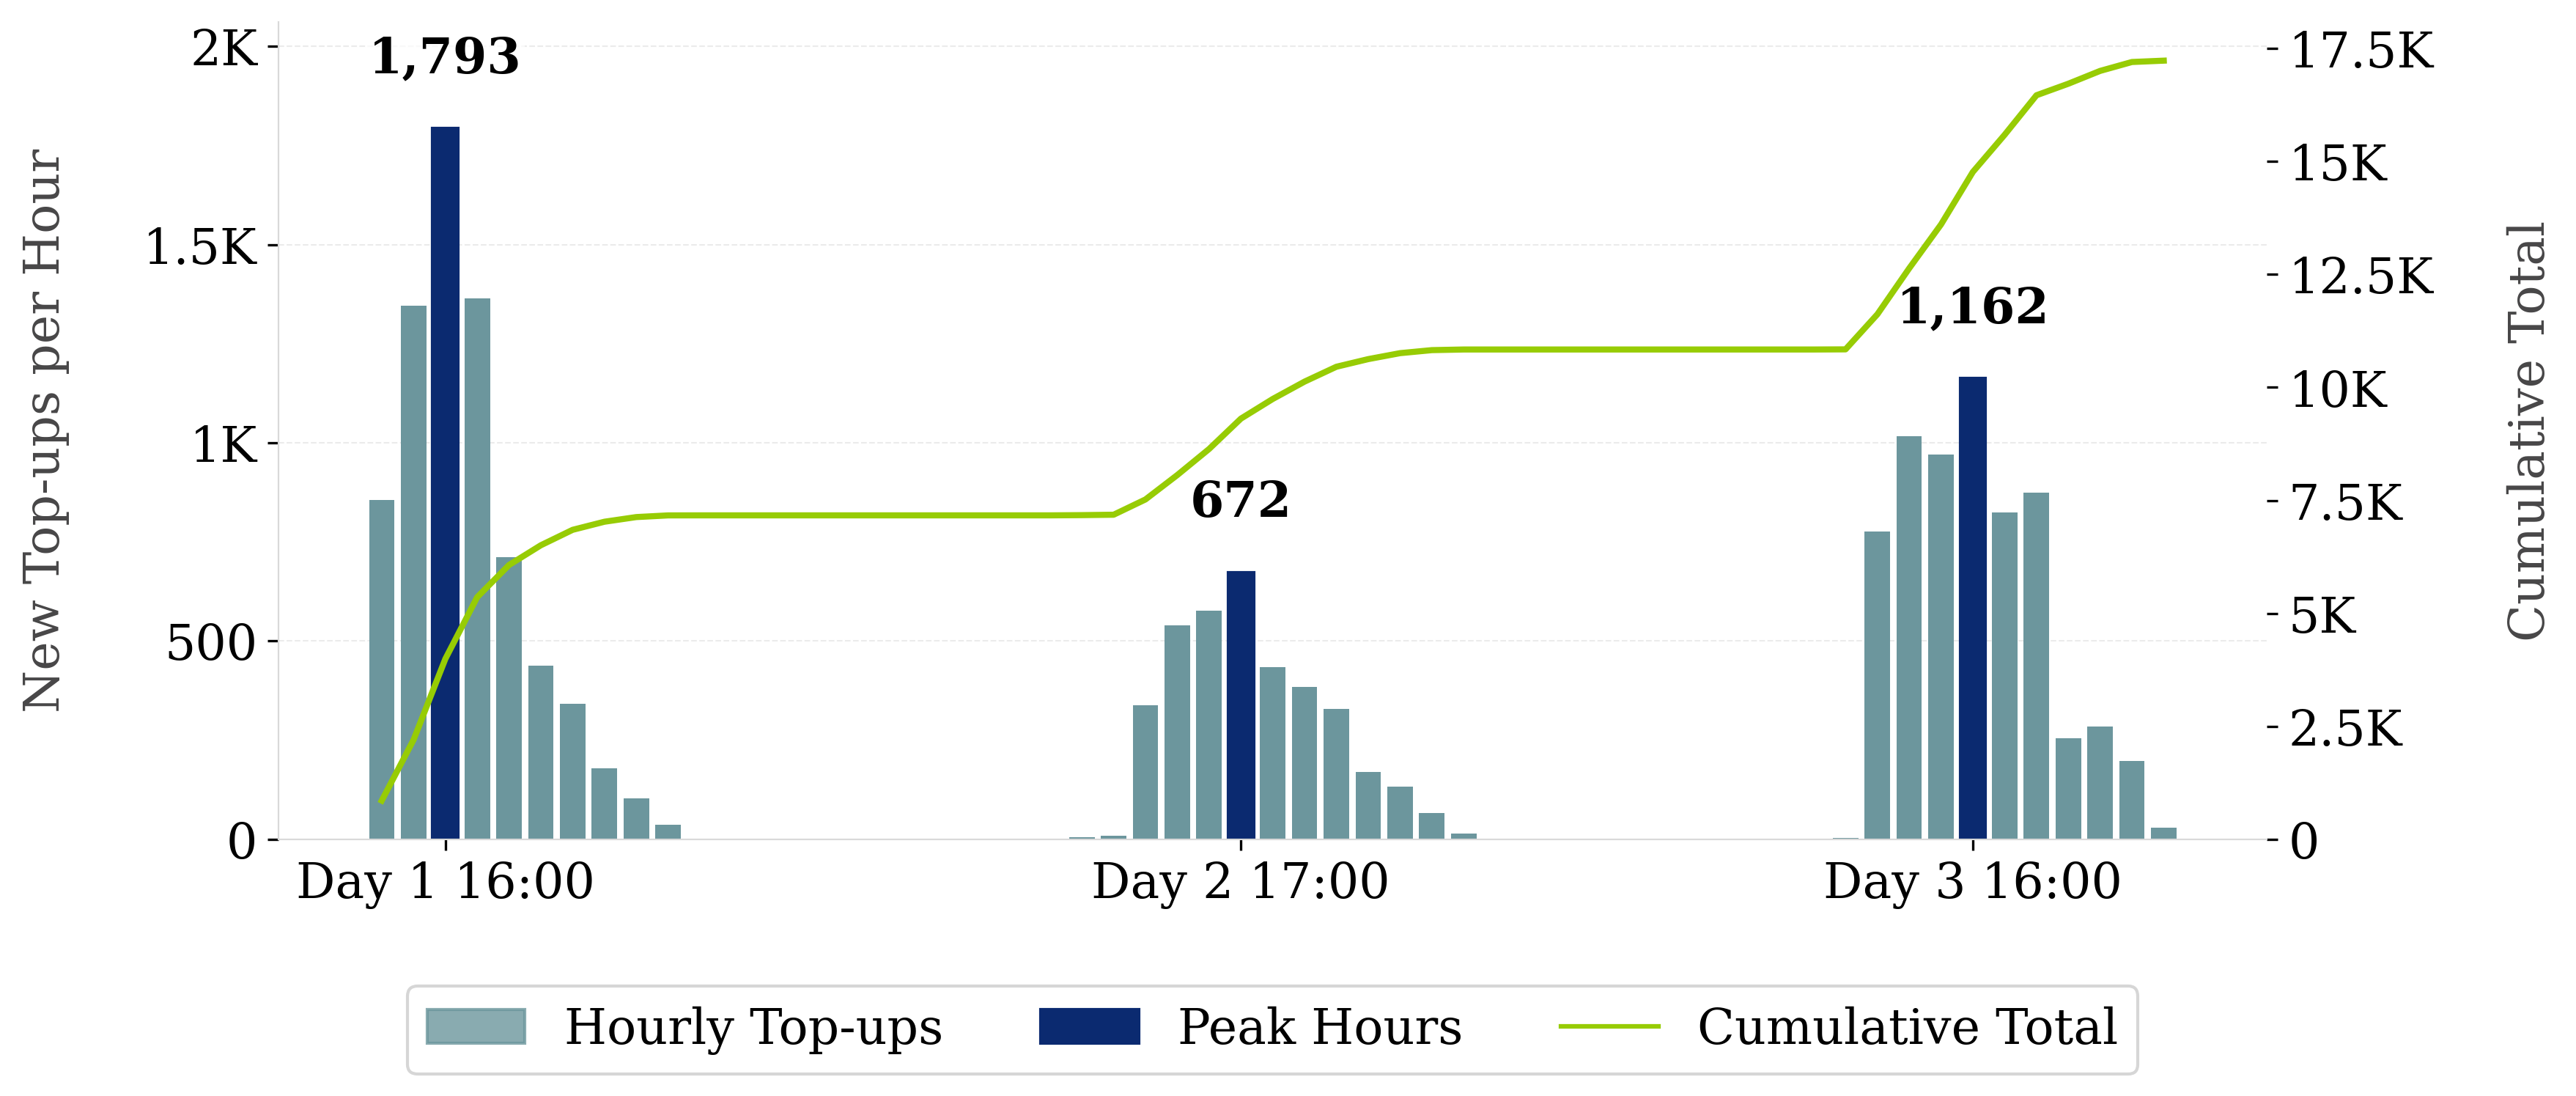
\includegraphics[width=\textwidth]{\ChartsDir/rq26-topup-patterns}
	\caption{\rqshorttext{customers-top-up-peaks} Credit Top-up Patterns During Event}
	\label{fig:topup-patterns}
	\source
\end{figure}

The data shows three major peak periods:
\begin{itemize}
	\item \textbf{Day 1 Peak}: The highest single-hour volume occurred at 16:00 with \bfmtnum{1793}~top-ups
	\item \textbf{Day 2 Peak}: A moderate peak at 17:00 with~\bfmtnum{672}~top-ups
	\item \textbf{Day 3 Peak}: A strong resurgence with~\bfmtnum{1162}~top-ups at 16:00
\end{itemize}

Each day had a similar pattern, with activity increasing in the early afternoon, peaking in the late afternoon (between 16:00 and 18:00), and gradually decreasing into the evening.
The overnight hours (00:00–12:00) saw minimal top-up activity.

\begin{keytakeaways}
	\begin{itemize}
		\item Peak top-up activity consistently occurred during late afternoon hours
		\item Day 1 saw the highest single-hour volume with \bfmtnum{1793} top-ups
		\item Clear daily pattern of afternoon peaks and overnight lulls
		\item Day 3 showed sustained high activity with multiple hours exceeding \bfmtnum{800} top-ups
	\end{itemize}
\end{keytakeaways}

%%% Customer / Segmentation Analysis
%%% --------------------------------------------------------------

\subsection{Customer Segmentation}
\label{subsec:analysis-customer-segmentation}

This section analyzes the distribution of customer types and their digital service adoption patterns, providing insights into how different groups of attendees interacted with the system.

\makerqbox{customers-top-up-online}

Out of~\bfmtnum{8974}~customers who got their chips through online ticket purchases, only \bfmtnum{1630}~(\bfmtnump[2]{18.20}\%) took advantage of the advance credit top-up option.
This indicates that while many customers purchased tickets online, most preferred to top up their credit on-site.

\makerqbox{customers-distribution-types}

The festival attracted a total of 10,009 attendees across different categories.
This distribution is shown in the~\autoref{fig:customer-distribution} below.

\begin{figure}[H]
	\centering
	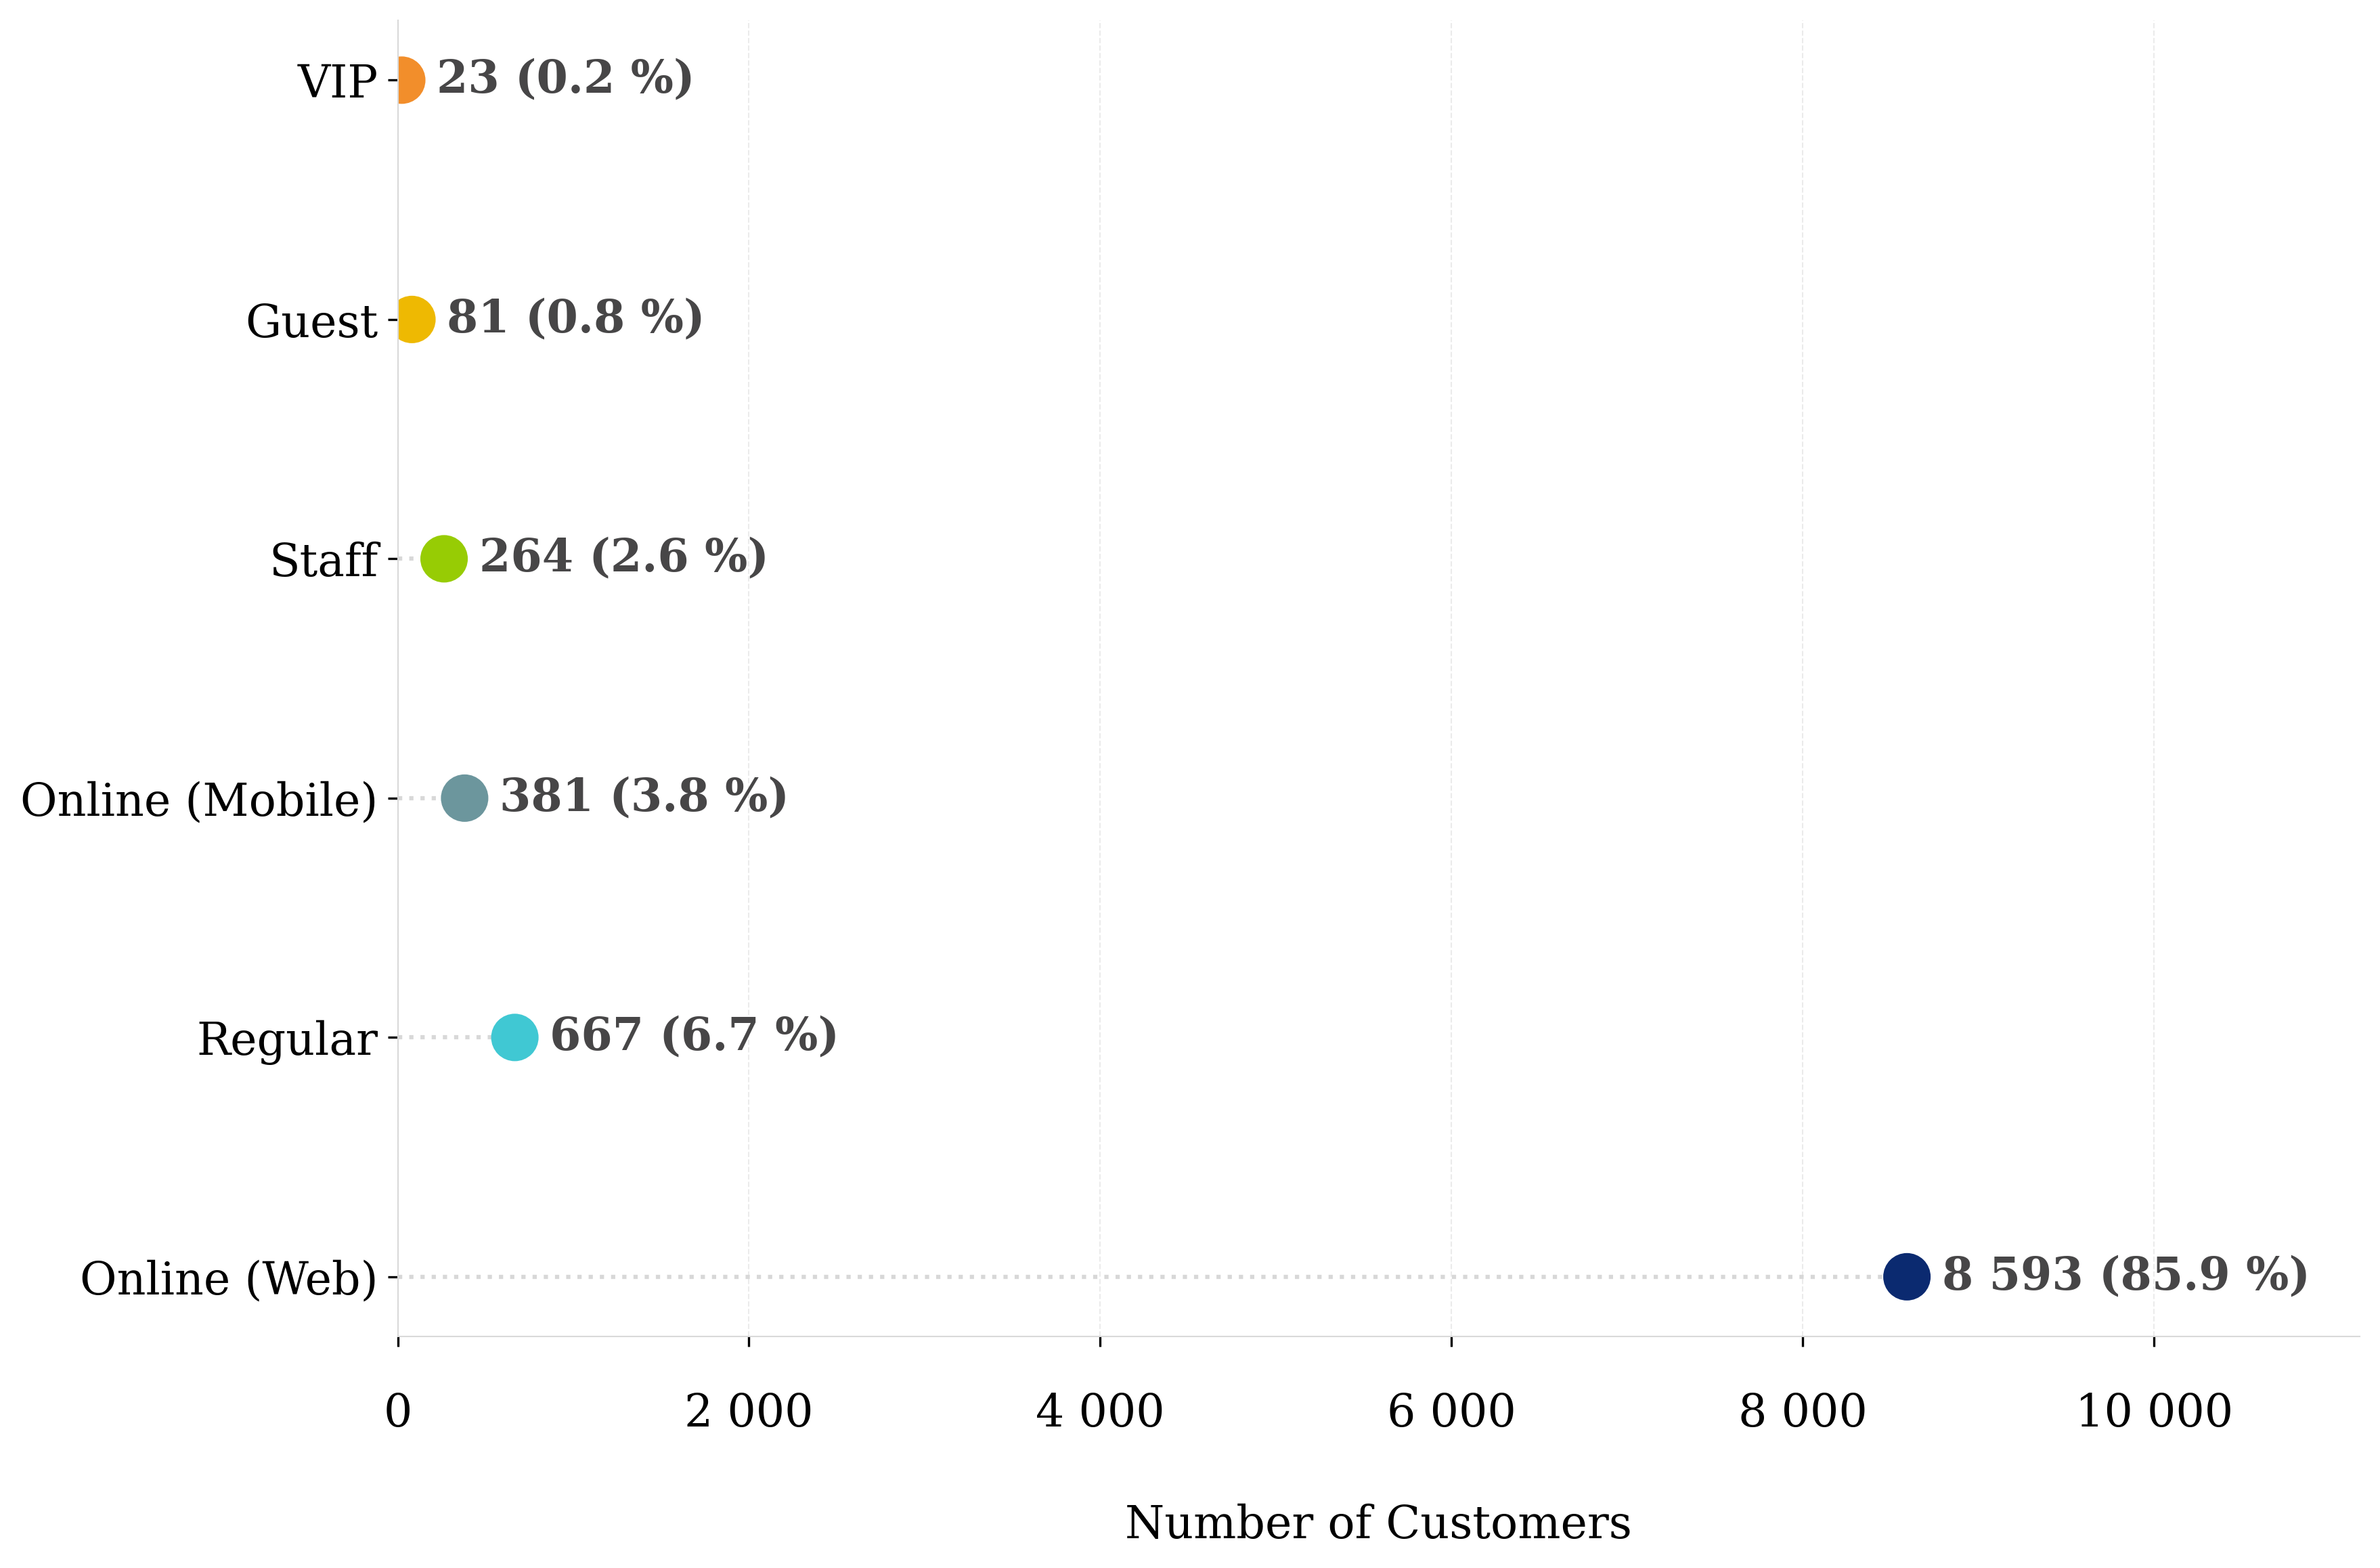
\includegraphics[width=\textwidth]{\ChartsDir/rq20-customer-distribution}
	\caption{\rqshorttext{customers-distribution-types} Customer Distribution by Type}
	\label{fig:customer-distribution}
	\source
\end{figure}

The data shows that the vast majority of attendees (\bfmtnump[2]{89.66}\%) came through online ticket purchases.
Regular on-site customers made up~\bfmtnump[2]{6.66}\%~of attendees, while staff, guests, and VIPs collectively accounted for less than~\bfmtnum{4}\%~of the total attendance.

\makerqbox{customers-mobile-app}

The festival provided multiple platforms for customers to interact with the system.
In the figure~\autoref{fig:customer-app-usage}~below is shown this breakdown.

\begin{figure}[H]
	\centering
	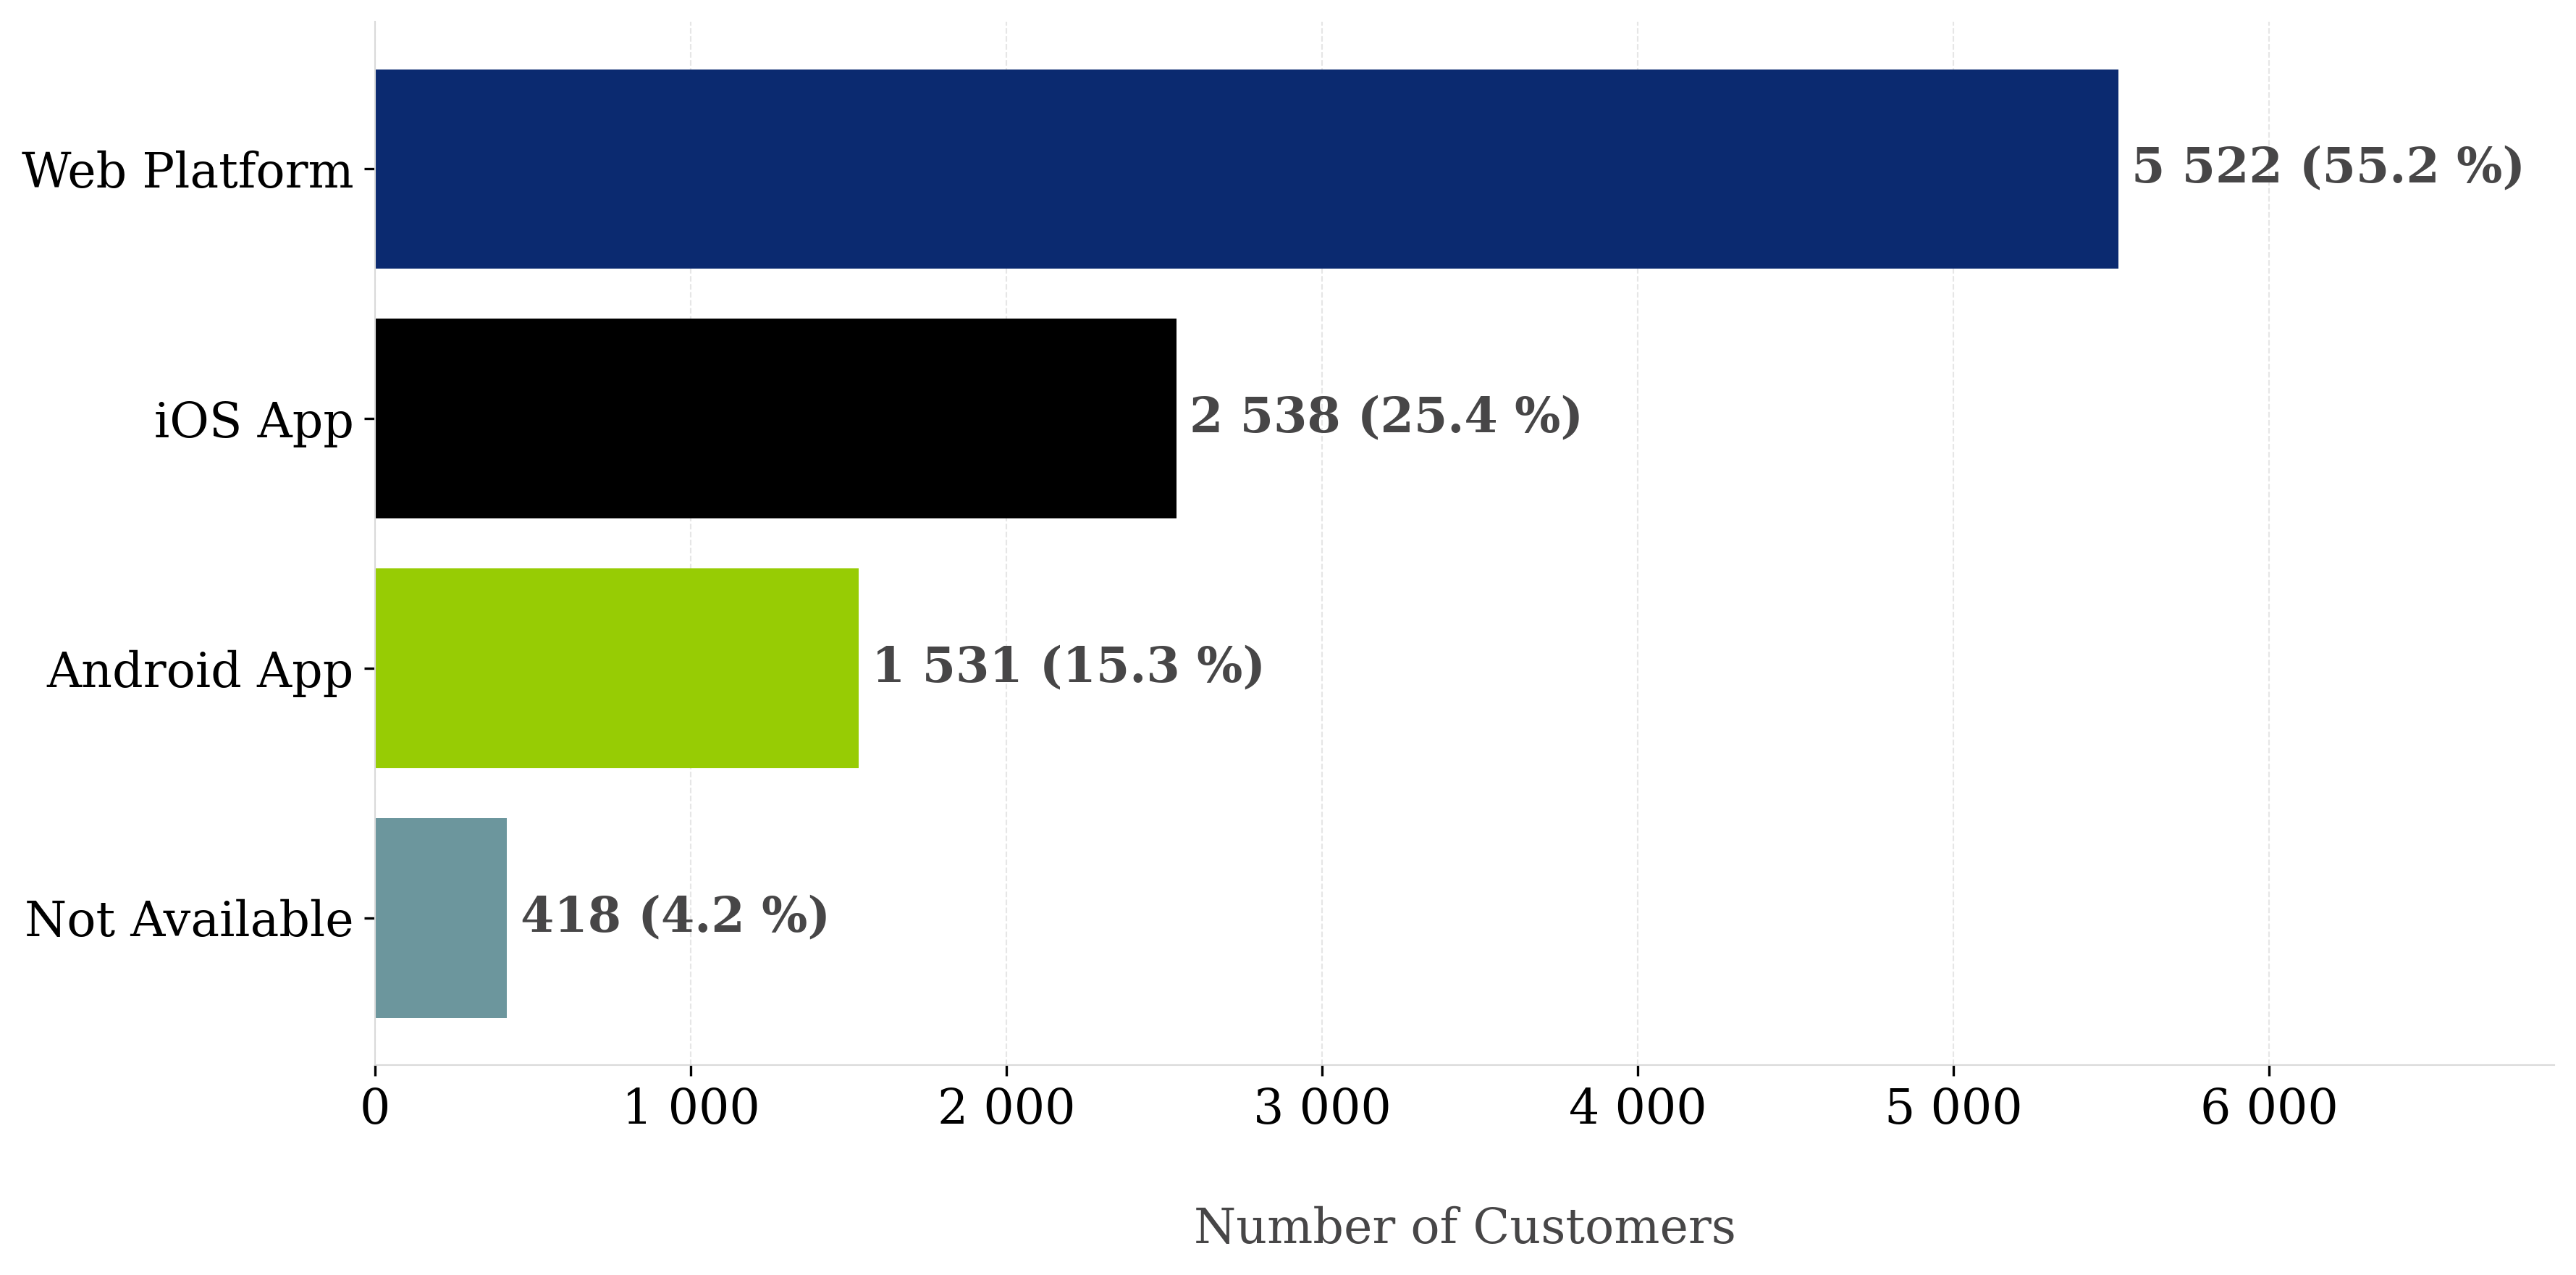
\includegraphics[width=\textwidth]{\ChartsDir/rq21-customer-app-usage}
	\caption{\rqshorttext{customers-mobile-app} Customer App Usage}
	\label{fig:customer-app-usage}
	\source
\end{figure}

The analysis reveals a significant adoption of mobile platforms, with~\bfmtnump[2]{40.69}\%~of customers using either iOS (\bfmtnump[2]{25.36}\%) or Android (\bfmtnump[2]{15.33}\%) mobile apps.
The web platform remained the most popular choice, used by~\bfmtnump[2]{55.17}\%~of customers.
A small portion (\bfmtnump[2]{4.14}\%) of customers had no recorded platform preference whatsoever.

\begin{keytakeaways}
	\begin{itemize}
		\item Only~\bfmtnump[2]{18.2}\%~of online ticket holders preloaded their credit before the event
		\item Online ticket purchases dominated attendance (\bfmtnump[2]{89.66}\%~of all customers)
		\item Mobile app adoption was substantial, with~\bfmtnump[2]{40.69}\%~of customers using mobile platforms
		\item iOS app usage (\bfmtnump[2]{25.36}\%) was notably higher than Android (\bfmtnump[2]{15.33}\%)
		\item The web platform remained the preferred choice for most customers (\bfmtnump[2]{55.17}\%)
	\end{itemize}
\end{keytakeaways}


%%% Customer / Payment Behavior Analysis
%%% --------------------------------------------------------------

\subsection{Payment Behavior Analysis}
\label{subsec:analysis-customer-payment-behavior}
This subsection focuses mainly on the payment segmentation and behavior of festival attendees.

By segmenting the customers based on their payment data,
such as their card issuing banks\footnote{Card Issuing bank is the bank responsible for issuing payment cards to customers. Issuers manage cardholder accounts, authorise transactions, and handle billing\cite{takepayments_what_are_card_schemes_and_how_do_they_work}.}~and
used payment card schemes\footnote{Card Scheme, such as Mastercard or Visa, are a payment network provider who processes card payments globally\cite{takepayments_what_are_card_schemes_and_how_do_they_work}.}~schemes,
the analysis should find interesting patterns and answer the defined research questions.

\makerqbox{customers-bank-cards}

The analysis of bank refunds reveals the distribution among Czech banking institutions shown in the~\autoref{fig:bank-refunds} below.

\begin{figure}[H]
	\centering
	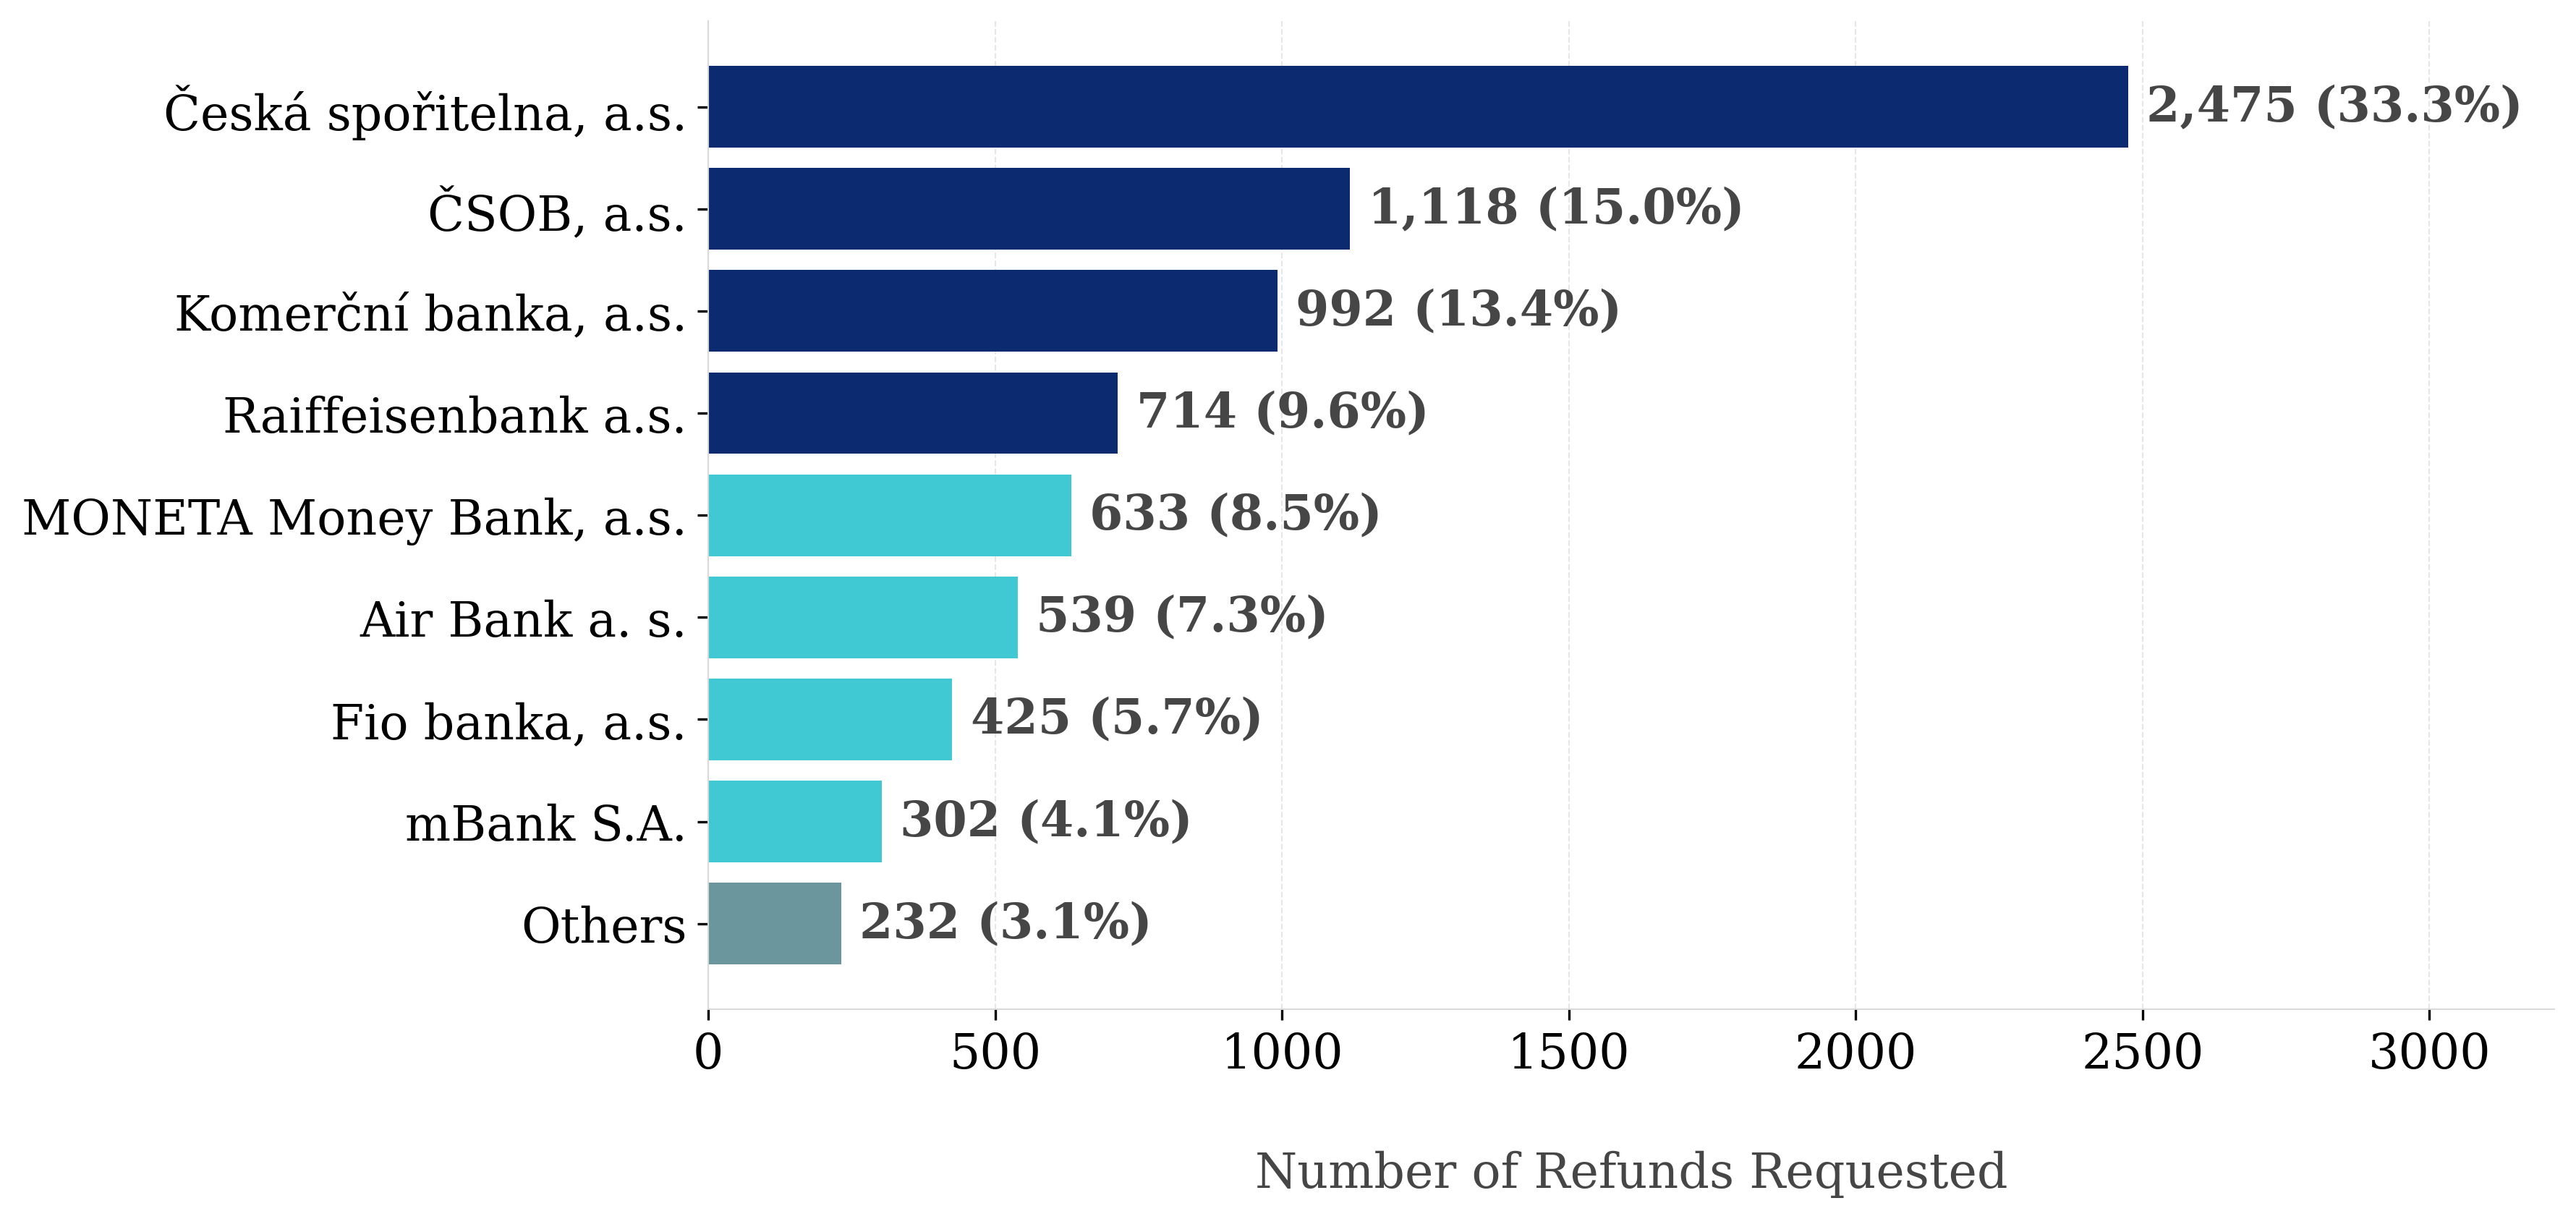
\includegraphics[width=\textwidth]{\ChartsDir/rq22-bank-refunds}
	\caption{\rqshorttext{customers-bank-cards} Bank Refunds Distribution}
	\label{fig:bank-refunds}
	\source
\end{figure}

Out of~\bfmtnum{7430}~online credit refunds that were requested, the data shows that \textbf{Česká spořitelna} was the leading bank, accounting for~\bfmtnump[1]{33.3}\%~of all refunds.
Followed by \textbf{ČSOB} and \textbf{Komerční banka} with~\bfmtnump[1]{15}\%~and~\bfmtnump[1]{13.4}\%~share respectively.

\makerqbox{customers-card-schemes}

\begin{figure}[H]
	\centering
	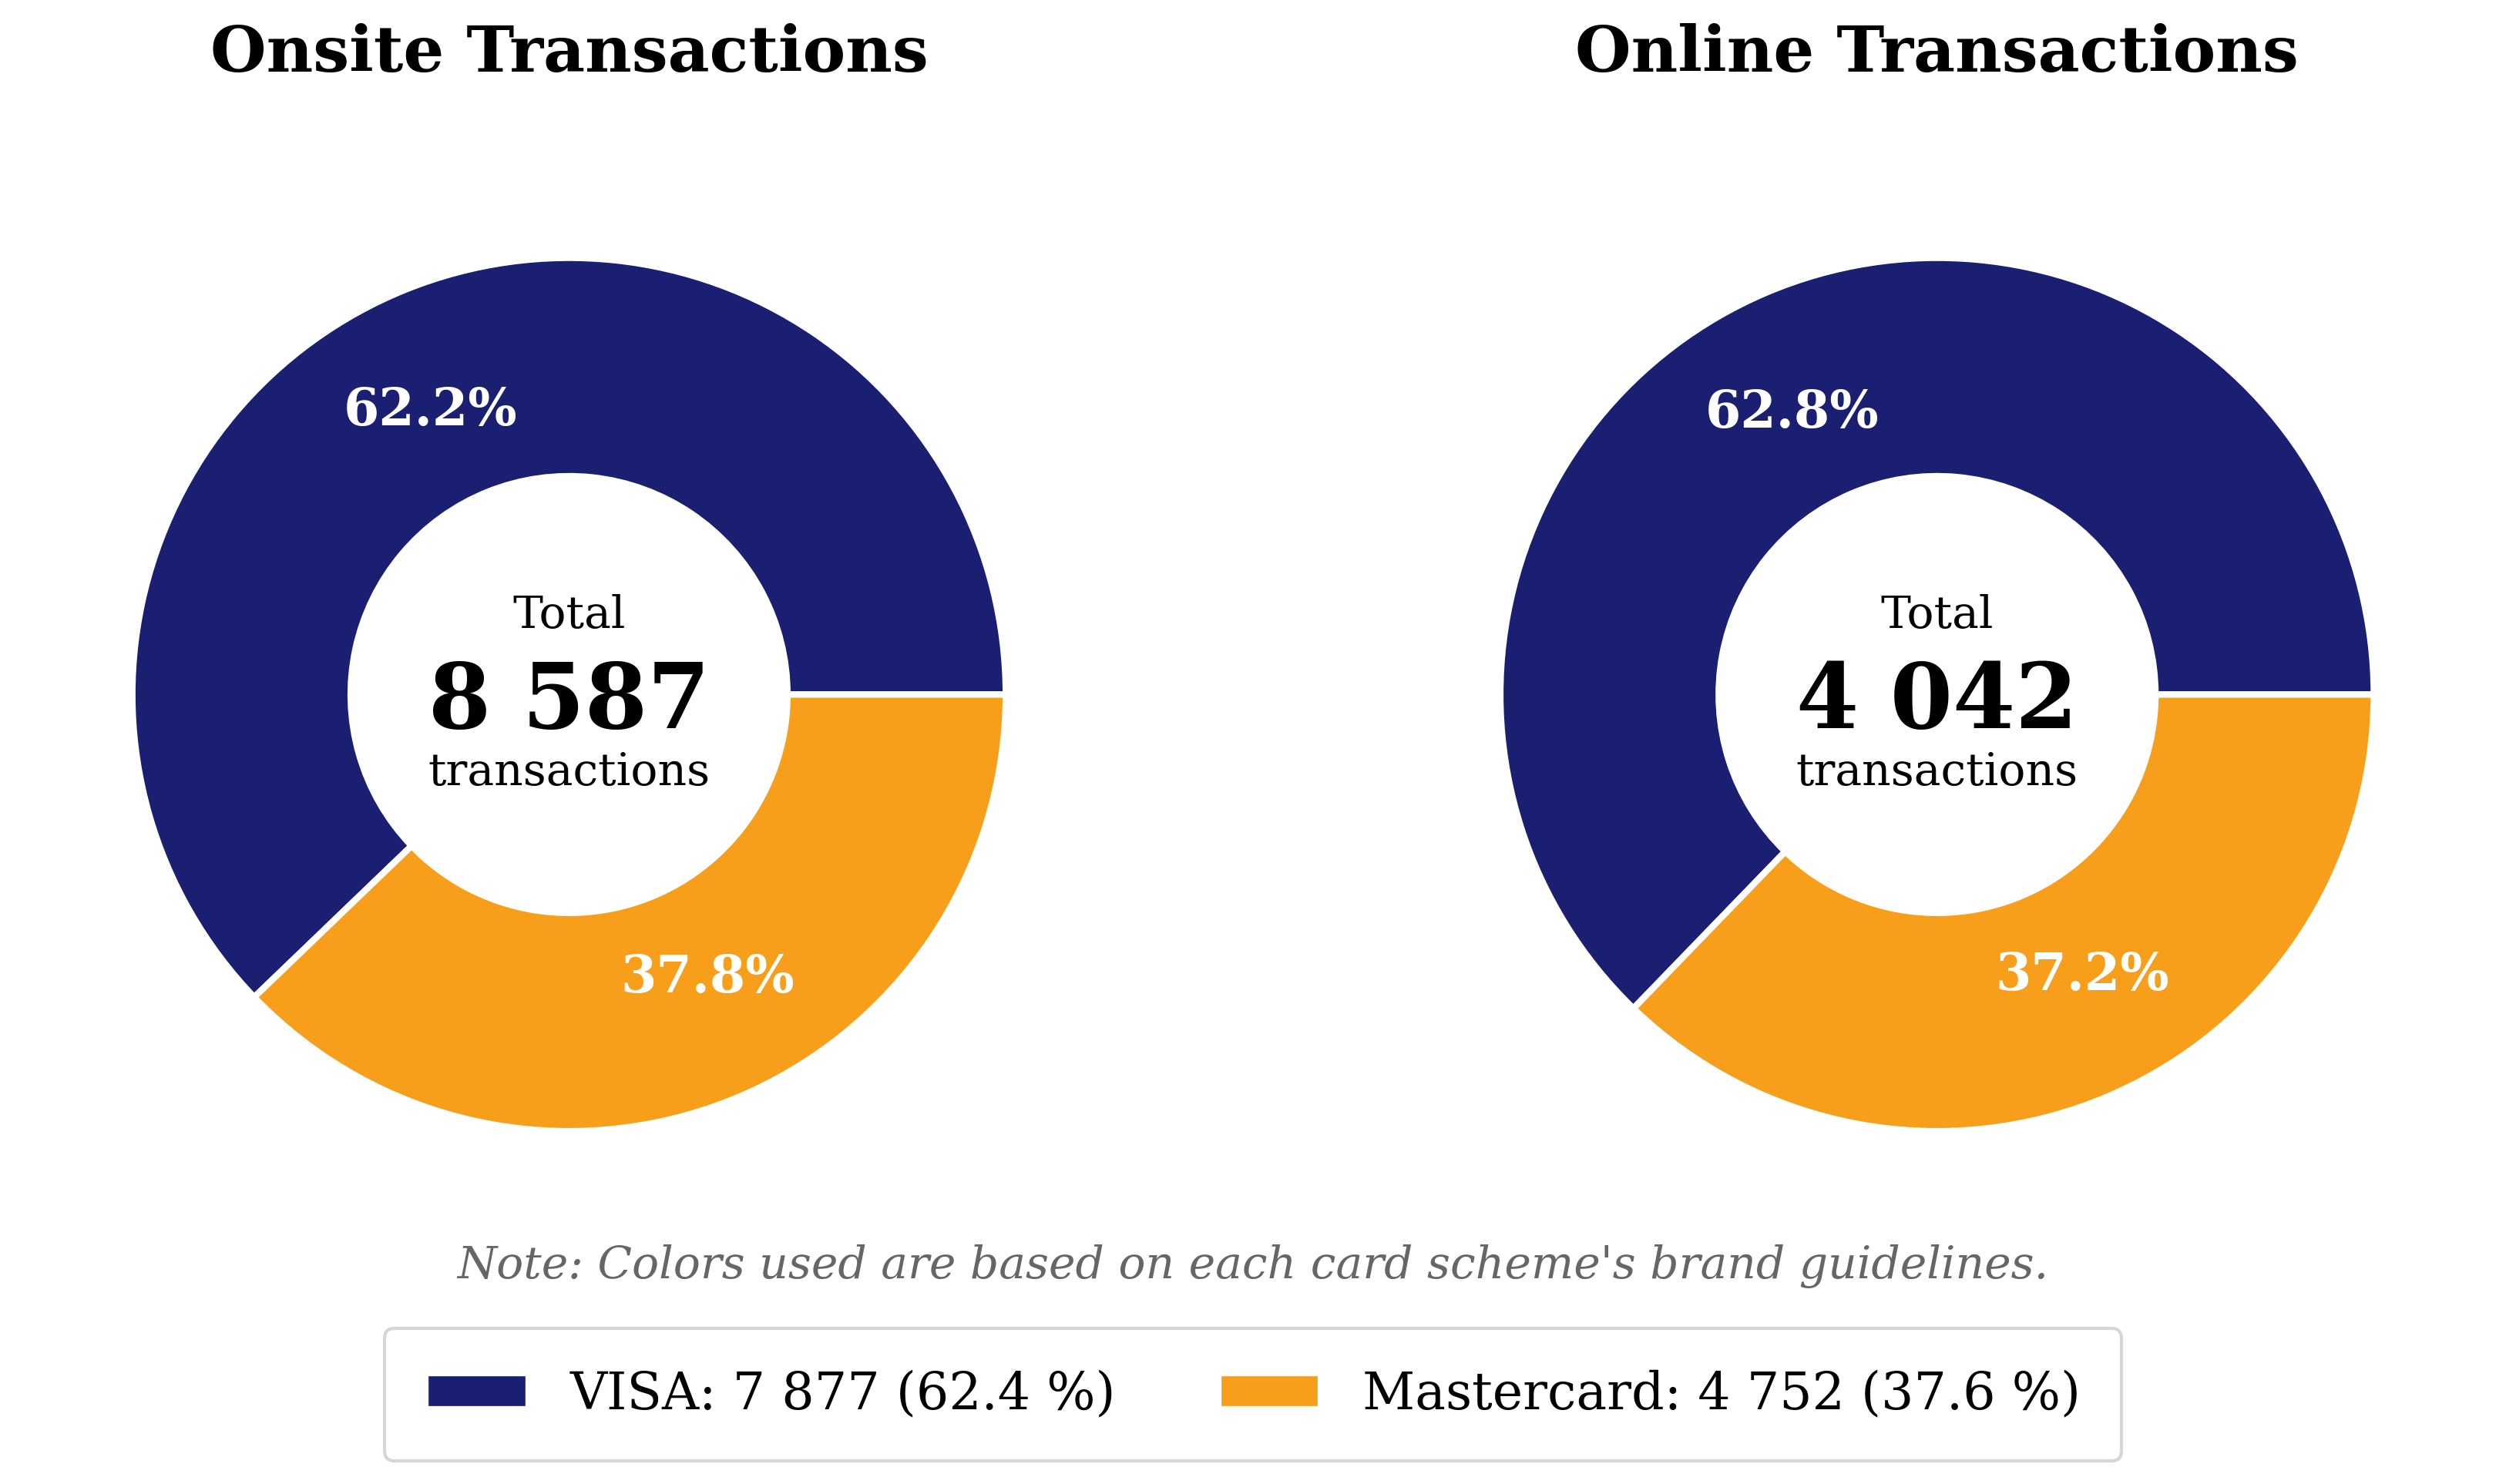
\includegraphics[width=\textwidth]{\ChartsDir/rq23-card-schemes}
	\caption{\rqshorttext{customers-card-schemes} Card Schemes Distribution}
	\label{fig:card-schemes}
	\source
\end{figure}

Out of total \bfmtnum{12626}~card transactions done both online (online ticket purchases, credit top-ups in advance) and onsite (onsite top-ups at festival, onsite physical ticket purchases), only two card schemes were identified:
\begin{itemize}
	\item \textbf{VISA} cards were used in~\bfmtnump[1]{62.4}\%~of transactions, making them the dominant card scheme.
	\item \textbf{Mastercard} cards followed at~\bfmtnump[1]{37.6}\%~of transactions.
\end{itemize}

This distribution rather nicely follows the local trend, where VISA is the most used card scheme with \bfmtnum{65}\%~market share and Mastercard with \bfmtnum{35}\%~market share\cite{spbk_czech_profil_karty}.

\makerqbox{customers-top-up-frequency}

Analyzing onsite top-up frequency behavior at the festival reveals the distribution of top-up counts among customers, as shown in the~\autoref{fig:top-up-behavior} below.

\begin{figure}[H]
	\centering
	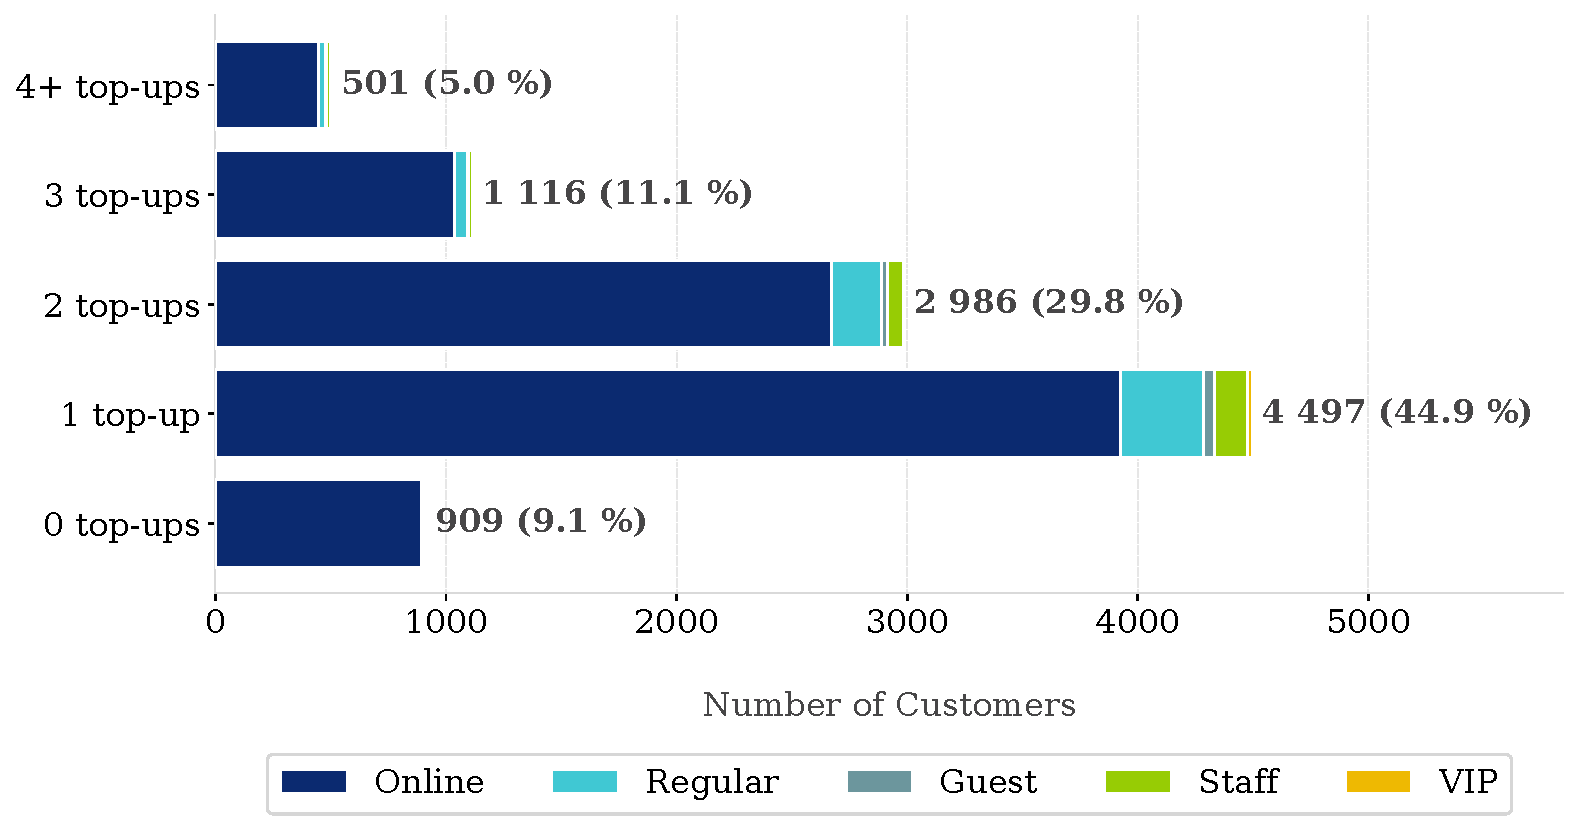
\includegraphics[width=\textwidth]{\ChartsDir/rq27-topup-frequency}
	\caption{\rqshorttext{customers-top-up-frequency} Top-up Behavior Analysis}
	\label{fig:top-up-behavior}
	\source
\end{figure}

The analysis of top-up behavior reveals that most customers (\bfmtnump[1]{44.9}\%) topped up only once during the festival.
A significant portion (\bfmtnump[1]{29.8}\%) topped up twice, while only a small fraction of customers (\bfmtnump[0]{5}\%) topped up more than three times.

Interesting finding is that around~\bfmtnump[0]{9}\%~of customers did not top up at onsite at all.
This meant for Online customers that they preloaded their credit before the event and did not need nor required to top up during the festival.

For other on-site registered customers, it meant they did not use their chip bracelet for payments at all, but only as an entry ticket or for access control purposes.

\begin{keytakeaways}
	\begin{itemize}
		\item The most common bank for refunds was \textbf{Česká spořitelna} (\bfmtnump[1]{33.3}\%)
		\item \textbf{VISA} cards were predominantly used (\bfmtnum{62}\%) compared to \textbf{Mastercard} (\bfmtnum{37}\%)
		\item The majority of customers (\bfmtnump[1]{74.7}\%) topped up their credit 1 or 2 times during the event
		\item Very few customers (\bfmtnum{5}\%) needed four or more top-ups
	\end{itemize}
\end{keytakeaways}

%%% Customer / Purchase Pattern Analysis
%%% --------------------------------------------------------------

\subsection{Purchase Pattern Analysis}
\label{subsec:analysis-customer-purchase-pattern}

This section examines customer purchase behaviors throughout the festival, focusing on beverage preferences across different times of day and common product combinations.

This section examines customer purchase behaviors throughout the festival, focusing on beverage preferences across different times of day and common product combinations.

%%% Customer / Purchase Pattern Analysis / Beverage Preferences

\subsubsection{Beverage Preferences Throughout the Day}
\label{subsubsec:analysis-beverage-preferences}

\makerqbox{customers-drink-preferences}

To analyze beverage preferences throughout the day, sales data was aggregated by hour and beverage category.
Figure~\ref{fig:beverage-preferences}~shows the distribution of alcoholic and non-alcoholic beverage sales over the course of the day.

\begin{figure}[H]
	\centering
	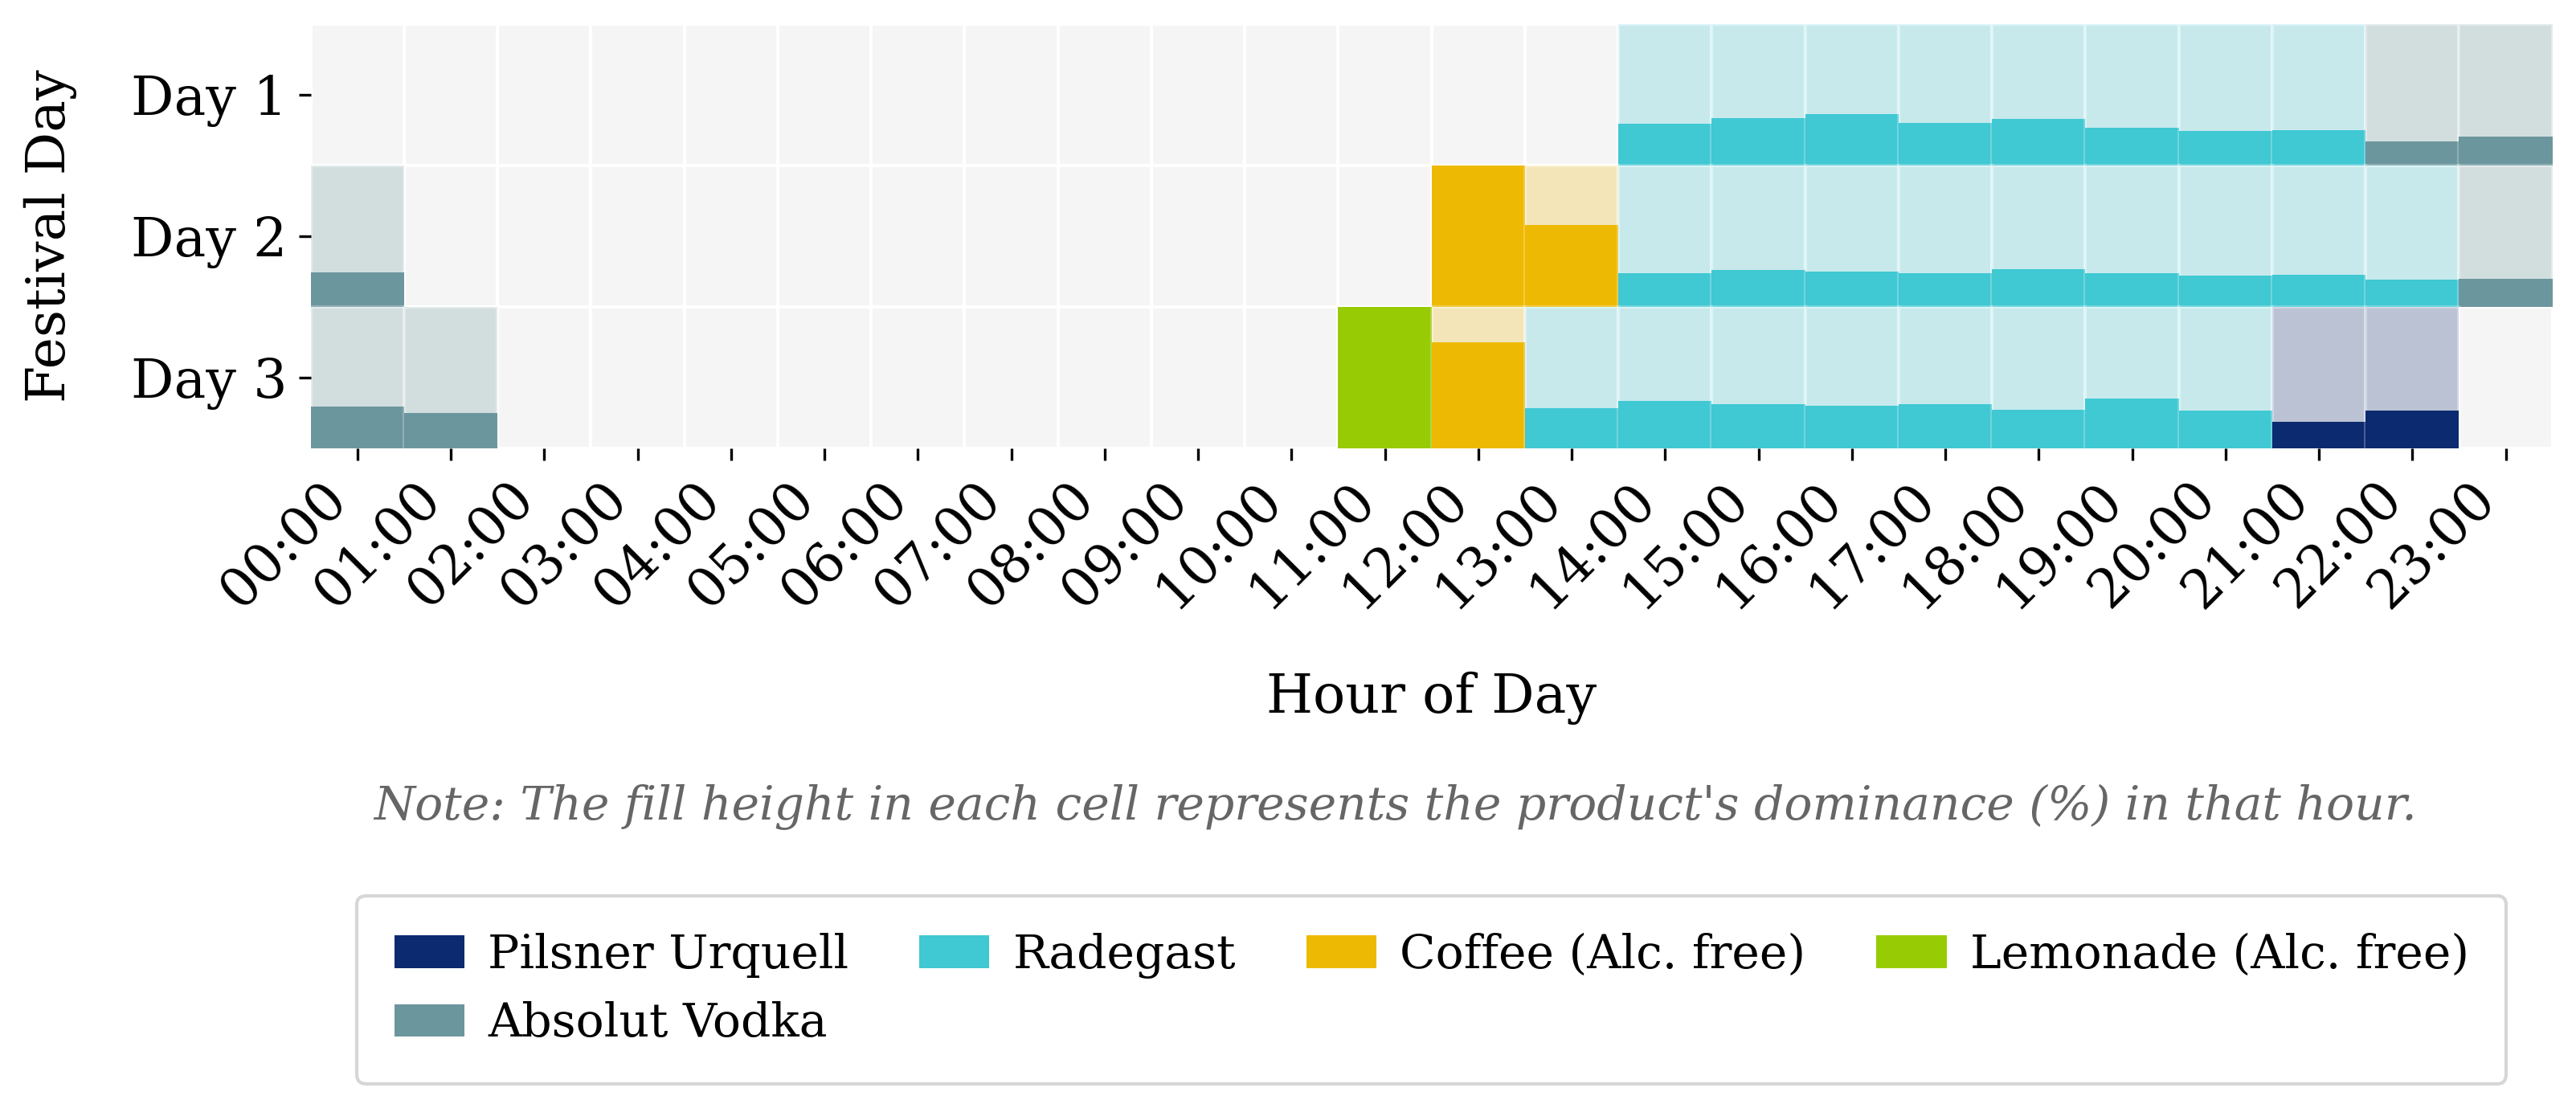
\includegraphics[width=\textwidth]{\ChartsDir/rq28-beverage-preferences}
	\caption{\rqshorttext{customers-drink-preferences} Beverage Preferences Throughout the Day}
	\label{fig:beverage-preferences}
	\source
\end{figure}

These results reveal that non-alcoholic beverages, such as Coffee and Lemonades, were most popular around noon.
Afternoon hours saw a shift towards light alcoholic beverages, with beer sales peaking in the late afternoon and early evening.

The beer preferences also show and confirm previous findings that Radegast was the most popular beer brand, with Pilsner Urquell following closely behind, especially at the end of the festival on Day 3.

Late evening hours saw a shift towards spirits and shots, with Absolut Vodka emerging as the most popular choice.

Hours without any preferences indicate that no sales were recorded during those times, or that the sales were too low (\(\leq 10\)~products sold in an hour) to be considered significant.

This showed no sales data throughout the night and early morning, which is expected.
However, one interesting observation is the lack of sales at the end of the festival on Day 3 after 22:00, which would indicate the festival's closing time.

\begin{infobox}{Why would a festival close at 22:00 on a Saturday?}
	The festival ended prematurely on Day 3 due to an unexpected change in weather, which later resulted in evacuation of the festival grounds.
\end{infobox}

This information was not possible to extract from the data alone, but it was a known fact from the festival organizer.

\begin{keytakeaways}
	\begin{itemize}
		\item Non-alcoholic beverages were most popular around noon.
		\item Beer sales peaked in the late afternoon and early evening.
		\item Radegast was the most popular beer brand throughout the festival.
		\item Absolut Vodka was the most popular spirit in the late evening.
		\item The festival ended prematurely on Day 3 due to an unexpected change in weather.
	\end{itemize}
\end{keytakeaways}

%%% Customer / Purchase Pattern Analysis / Common Product Combinations

\subsubsection{Common Product Combinations}
\label{subsubsec:analysis-common-combinations}

\makerqbox{customers-common-combinations}

Identifying frequently purchased product combinations can provide valuable insights into customer preferences and behavior.
Two analyses were performed: one with returnable cups and one without, as the high frequency of cup purchases can obscure other meaningful patterns.

The initial results are shown in the~\autoref{fig:common-combos-with-cups}~below and ss expected, returnable cups appear prominently in the most popular combinations as it was necessary to purchase them for drinks.

\begin{figure}[H]
	\centering
	\small
	% table
	\begin{tabularx}{\textwidth}{
		|>{\columncolor{unicorn_blue!5}}X
		|>{\columncolor{unicorn_blue!5}}X
		|>{\columncolor{unicorn_blue!5}}r
		|>{\columncolor{unicorn_blue!5}}r|
	}
		\hline
		\rowcolor{unicorn_blue}
		\textbf{\color{white}Product A}
		& \textbf{\color{white}Product B}
		& \textbf{\color{white}Count}
		& \textbf{\color{white}\% of total}
		\\
		\hline
		\csvreader[
		head to column names,
		late after line= \\,
		filter={\thecsvinputline<9}
		]{\DataDir/rq29-product-combos-with-returnable.csv}{
			product1=\producta,
			product2=\productb,
			combination_count=\combos,
			percentage_of_all_transactions=\percentage
		}{
			\producta
			& \productb
			& \num[group-separator={,}]{\combos}
			& \num[round-precision=2]{\percentage}\%
		}
		\hline
	\end{tabularx}
	% space
	\par\vspace*{0.5em}
	% treemap
	
\includegraphics[width=\textwidth]{\ChartsDir/rq29-product-combos-with-returnable}
	\caption{\rqshorttext{customers-common-combinations} Most Common Product Combinations with Cups}
	\label{fig:common-combos-with-cups}
	\source
\end{figure}


To gain additional insights, the analysis was repeated while excluding returnable cups, as shown in the~\autoref{fig:common-combos-without-cups}~below.

\begin{figure}[H]
	\centering
	\small
	% table
	\begin{tabularx}{\textwidth}{
		|>{\columncolor{unicorn_blue!5}}X
		|>{\columncolor{unicorn_blue!5}}X
		|>{\columncolor{unicorn_blue!5}}r
		|>{\columncolor{unicorn_blue!5}}r|
	}
		\hline
		\rowcolor{unicorn_blue}
		\textbf{\color{white}Product A}
		& \textbf{\color{white}Product B}
		& \textbf{\color{white}Count}
		& \textbf{\color{white}\%~of~total}
		\\
		\hline
		\csvreader[
		head to column names,
		late after line= \\,
		filter={\thecsvinputline<9}
		]{\DataDir/rq29-product-combos-without-returnable.csv}{
			product1=\producta,
			product2=\productb,
			combination_count=\combos,
			percentage_of_all_transactions=\percentage
		}{
			\producta
			& \productb
			& \num[group-separator={,}]{\combos}
			& \num[round-precision=2]{\percentage}\%
		}
		\hline
	\end{tabularx}
	% space
	\par\vspace*{0.5em}
	% treemap
	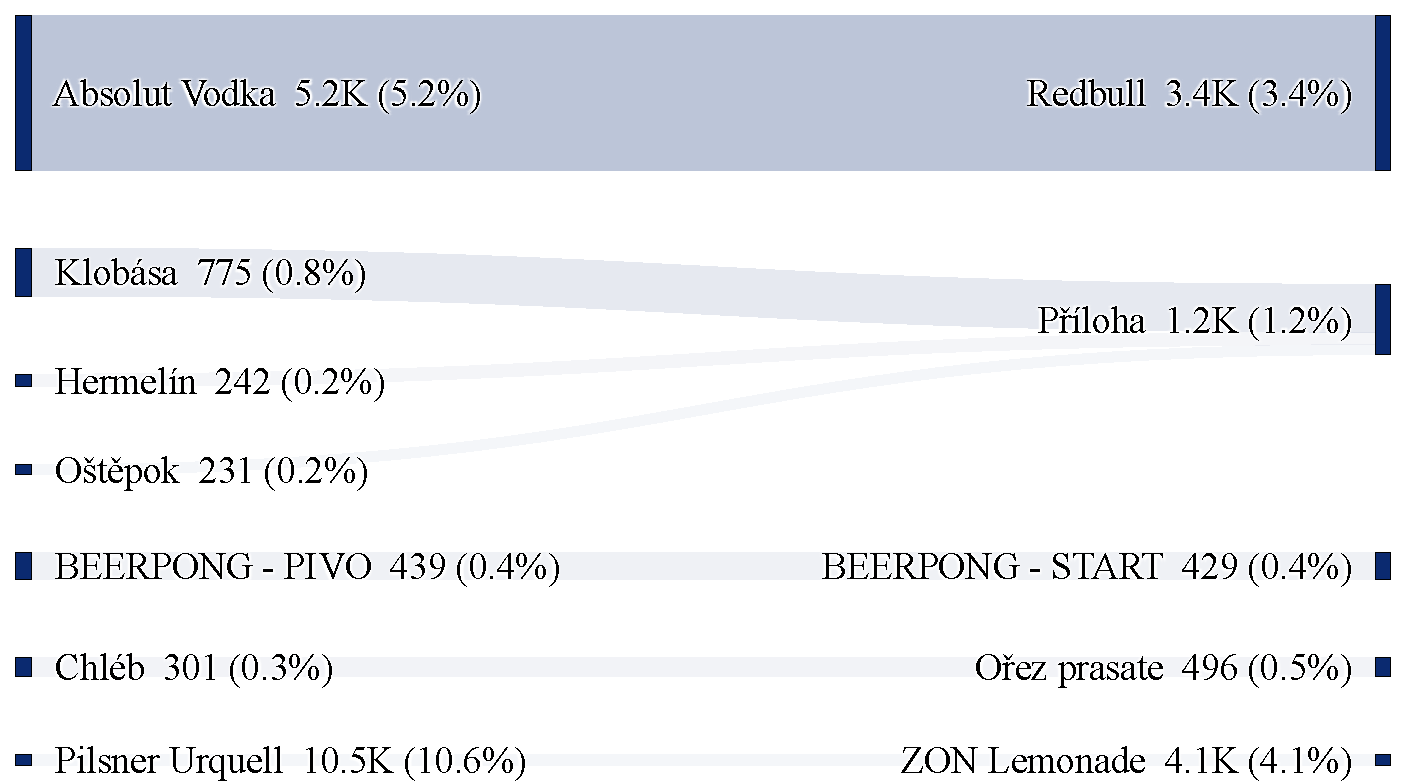
\includegraphics[width=\textwidth]{\ChartsDir/rq29-product-combos-without-returnable}
	\caption{\rqshorttext{customers-common-combinations} Most Common Product Combinations without Cups}
	\label{fig:common-combos-without-cups}
	\source
\end{figure}

This revealed the most popular product combination, without returnable cups included, was the \textbf{Absolut Vodka} and \textbf{Redbull} accounting to total of~\bfmtnump[2]{2.48}\%~of all transactions.

There was also a notable high-combination of non-beverage products, such as \textbf{Klobása}, \textbf{Hermelín} or \textbf{Oštěpok} in combination with \textbf{Příloha} making it a seemingly popular food choice.

Interpretation of the results could have been done in many ways, for example, using a network graph to visualize the relationships between products.
This, as exciting as it sounded, was not in the end the most suitable way to present the results in a clear and concise manner.

\begin{keytakeaways}
	\begin{itemize}
		\item The most common product combination was \textbf{Absolut Vodka} and \textbf{Redbull} (\bfmtnump[2]{2.48}\%~of all transactions)
		\item The most common non-beverage combination was \textbf{Klobása} and \textbf{Příloha}
		\item Returnable cups were, not surprisingly, a significant part of the most common combinations
	\end{itemize}
\end{keytakeaways}

\subsection{Summary}
\label{subsec:analysis-customer-summary}

This section provided a thorough evaluation of festival attendees' habits, preferences, and segmentation.
It provided practical information about visitor interactions with the festival by analyzing trends in attendance, payment methods, purchase preferences, and event product combinations that contributed most to overall sales.

All previously defined questions were answered and presented in a simple and understandable way, providing hopefully valuable insights for the festival organizer.

%%% Section: Conclusion
%%% --------------------------------------------------------------


\section{Conclusion}
\label{sec:analysis-conclusion}

The analyses in this chapter provide a comprehensive look at the festival's behavior, including data-driven insights on operational effectiveness, financial performance, and customer behavior.
By fully addressing every research question, the results provide an in-depth knowledge of the festival dynamics and offer practical suggestions for upcoming seasons.

Analysis of cash flow dynamics and income sources revealed important revenue-generating systems and their interactions.
Concurrent with this, performance indicators showed the system's ability to control transactional spikes and identified possible bottlenecks.

Examination of consumer behavior revealed notable trends in attendance and buying preferences.

Furthermore, the study of beverage consumption highlighted how important brands and product categories are for determining sales.
The distinctive trends in beverage preferences and their correlation with specific times of day highlight the possibility to adapt offers to satisfy consumer needs.

The foundation for the upcoming dashboard development—which will show consolidated results in an interactive and user-centric form—is laid in this chapter.


	% ✅ chapter - implementation of the analytical dashboard
	%%% Dashboard Implementation
%%%%%%% Wording: ⏳
%%%%%%% Styling: ⏳
%%%%%%% References: ⏳
%%%%% Grammar: ⏳
%%% --------------------------------------------------------------
\chapter{Dashboard Implementation}
\label{ch:dashboard-implementation}

This chapter describes the implementation of a prototype analytical dashboard that visualizes the key findings from the analysis.
Using Dash and Plotly\footnote{Dash is a Python web application framework that enables the creation of interactive web applications using Plotly visualizations\cite{plotly_dash_plotly_com}.},
we developed a local development prototype that demonstrates how the analytical insights could be presented in an interactive format.
The implementation focused on efficient data querying, caching strategies for development, and handling asynchronous operations in Python.

The chapter details the technical approach, the challenges encountered during implementation (particularly with callback caching and async handling), and our solutions to these challenges.
While not intended for production deployment, the prototype successfully demonstrates the potential of the analytical findings in an interactive format.

%%% Section: Development Approach
%%% --------------------------------------------------------------
\begin{section}{Development Approach}
	\label{sec:implementation-development-approach}

	The implementation phase focused on transforming the analysis results from the~\autoref{ch:data-analysis-and-results} into an interactive dashboard prototype.
	Our approach prioritized rapid development and effective visualization of our analytical findings.

	\begin{subsection}{Development Goals}
		\label{subsec:implementation-development-approach-goals}

		The primary goal was to create a functional prototype dashboard that could effectively present our analysis results in an interactive format.
		Specifically, we aimed to:
		\begin{itemize}
			\item Demonstrate key findings through interactive visualizations
			\item Implement basic filtering capabilities for data exploration
			\item Create a responsive interface that handles data operations efficiently
			\item Establish a foundation for visualizing festival transaction data
		\end{itemize}

	\end{subsection}

	\begin{subsection}{Technology Selection}
		\label{subsec:implementation-development-approach-technology}

		The dashboard was build using Dash and Plotly, chosen primarily for their familiarity from prior personal experience in the academic field and their great capability for relatively fast data app prototyping\cite{plotly_dash_plotly_com}.

		The technology stack included:
		\begin{itemize}
			\item Dash \& Plotly\footnote{\url{https://dash.plotly.com/}} using Python for the core dashboard framework
			\item Dash Mantine Components\footnote{\url{https://www.dash-mantine-components.com}} for enhanced UI elements
			\item PostgreSQL\footnote{\url{https://www.postgresql.org/}} for local data storage
		\end{itemize}

		This stack was chosen specifically for prototyping, with Dash and Plotly providing a good balance of functionality and development speed based on previous personal experience using these tools in university projects.
		Mantine Components were added to enhance the visual presentation without significantly increasing additional development time.
	\end{subsection}

	\begin{subsection}{Local Development Focus}
		\label{subsec:implementation-development-approach-local}

		The dashboard was developed exclusively for local environment, focusing on demonstrating analytical capabilities rather than production readiness.

		This decision was influenced by several factors:
		\begin{itemize}
			\item The prototype nature of the implementation, focusing on demonstrating analytical insights rather than production features
			\item Complexity of Python async handling, production requirements and deployment challenges with Python environments
			\item Implementing a fully featured production-ready dashboard would require significant additional development time and would not bring additional value to the project
		\end{itemize}

		Moreover, as stated previously, the personal motivation for this thesis was to learn more about the data and demonstrate the findings in an interactive way, leading to more insights and knowledge for future updates of the NFCtron Hub dashboard.

	\end{subsection}
\end{section}

%%% Section: Core Architecture
%%% --------------------------------------------------------------
\begin{section}{Core Architecture}
	\label{sec:implementation-core-architecture}

	Since it was developed for local use only, it did not require any complex environmental setups for the app nor the database.
	This significantly simplified and sped up the development process, allowing us to focus on the core functionality and visual presentation of the dashboard.

	The dashboard's architecture was designed to efficiently manage data during development, with a strong emphasis on query management and caching strategies.

	\begin{subsection}{Query Management System}
		\label{subsec:implementation-core-architecture-query-management}

		To manage the SQL database interactions efficiently, a simple \textbf{Query Management System} has been implemented to handle loading data from our SQL database.

		It consisted of several key components:
		\begin{itemize}
			\item \textbf{QueryDefinition}: Defines query structure and parameters
			\item \textbf{QueryRegistry}: Maintains registered queries
			\item \textbf{QueryManager}: Handles query execution and caching
			\item \textbf{QueryParameter}: Defines parameter types and validation
		\end{itemize}

		The following example in~\autoref{lst:dashboard-implementation-query-management} demonstrates the query registration process:

		\begin{listing}[H]
			\caption{Query Management Example}
			\begin{minted}[breaklines]{python}
query_manager.registry.register_query(
    QueryDefinition(
        name="sankey_diagram",
        sql=QueryManager.process_sql_query("""
            SELECT * FROM get_sankey_diagram_data(:date_from$1, :date_to$2)
        """),
        parameters=[
            QueryParameter("date_from", datetime.datetime),
            QueryParameter("date_to", datetime.datetime)
        ],
        default_data="FSCacheDefault"  # Enables local CSV caching
    )
)
			\end{minted}
			\label{lst:dashboard-implementation-query-management}
		\end{listing}

		This class has been the core of the dashboard's data management, allowing multiple approaches to data loading and caching strategies.

		It allowed defining raw SQL queries with \texttt{QueryManager\.process\_sql\_query}, which safely handled parameter substitution and query formatting.
		Or it could have loaded SQL query from an external file (due to the complexity of the query) and then executed it with parameters.

		On top of that, it allowed for defining default data loading strategies, such as loading data from a local CSV cache, which significantly sped up the development process.
		More to this is described in the following section.
	\end{subsection}

	\begin{subsection}{Dual Caching Strategy}
		\label{subsec:implementation-core-architecture-caching}

		For the purpose of optimizing the development process, the implementation utilizes two caching mechanisms that are complementary to one another.

		\begin{subsubsection}{Query Result Caching}
			\label{subsubsec:implementation-core-architecture-query-cache}

			Since the dashboard relies on several complex SQL queries to load data, it was crucial to optimize query execution during development.
			Running these queries repeatedly during development significantly slowed down the development process.

			Thus, a very simple file-based caching system was implemented to store query results as CSV files, preventing redundant database queries during development.
			It, simply by defining a \texttt{default\_data} parameter in the \texttt{QueryDefinition} class, allowed to turn on the caching for specific queries which did not need to be reloaded every time.

			The query execution handler shown in~\autoref{lst:dashboard-implementation-query-cache} below\footnote{
				The implementation is rather a simplified pseudo-implementation, as the \texttt{execute\_query} method is more complex and contains additional logic for results formatting, database connection retries and error handling.
			}, demonstrates the simple implementation of this caching strategy.

			\begin{listing}[H]
				\caption{Query Result Caching Implementation}
				\begin{minted}[breaklines]{python}
def execute_query(self, query_name: str, parameters: Dict[str, Any], or_query_def: Optional[QueryDefinition]):
    query_key = self.get_query_key(query_name, parameters)

    if query_def.default_data == "FSCacheDefault":
        try:
            return pd._read_csv_cache(query_key)
        except Exception:
            pass

    # Execute database query directly
    result = self._execute_db_query(query_def, parameters)

    # Cache result for future use
    try:
        self._save_csv_cache(query_key, result)
    except Exception as e:
        print(f"Failed to save query {query_name} to cache: {e}")

    return result
				\end{minted}
				\label{lst:dashboard-implementation-query-cache}
			\end{listing}

			It firstly generates a unique query key based on the query name and its parameters in a form of hash, which then later was used as a directory and file path to the cached CSV data.

			Then if the caching is enabled for the query, it tries to read the CSV file from the cache directory and return it as a result.
			Otherwise, it exectures the DB query directly as usual and then saves the result to the cache directory for future use.
		\end{subsubsection}

		\begin{subsubsection}{Background Callback Caching}
			\label{subsubsec:implementation-core-architecture-callback-cache}

			Since the dashboard, when not using cached data, relied on long-running data processing operations, it was crucial to use Dash's background callbacks feature.
			These background callbacks run in a separate background proceses in a queue, allowing the main Dash application to remain responsive while the callback processes the data and then returns the result to the main application\cite{plotly_dash_plotly_com_background_callbacks}.

			Dash provides two options for background callback backends:

			\textbf{DiskCache}: Runs the callback logic in a separate process and stores the results to disk using the diskcache library.
			This is the easiest backend to use for local development but is not recommended for production.

			\textbf{Celery}: Runs the callback logic in a Celery worker\cite{celery_userguide_workers} and returns results to the Dash app through a Celery broker like Redis.
			This is recommended for production as it queues the background callbacks, running them one-by-one in the order that they were received by dedicated Celery worker(s).

			For our development purposes, we used the DiskCache backend, as it was easier to set up and use for local development:

			\begin{listing}[H]
				\caption{DiskCache Background Callback Manager Setup}
				\begin{minted}[breaklines]{python}
CACHE_DIR = os.path.join(os.path.dirname(__file__), 'dash_cache')
os.makedirs(CACHE_DIR, exist_ok=True)
# cache configuration
cache = diskcache.Cache(
	directory=CACHE_DIR,
	size_limit=3e9,
	eviction_policy='least-recently-used',
)

# unique launch_uid to refresh cache when the app restarts
launch_uid = uuid4()
background_callback_manager = dash.DiskcacheManager(
	cache,
	cache_by=[lambda: launch_uid],
	expire=300
)
				\end{minted}
				\label{lst:dashboard-implementation-callback-cache}
			\end{listing}

			This implementation evolved through several iterations as we encountered scaling challenges.
			More on this is later described in the~\autoref{sec:implementation-technical-challenges}.
		\end{subsubsection}
	\end{subsection}

	\begin{subsection}{Custom Callback Management System}
		\label{subsec:implementation-core-architecture-callbacks}

		While developing the dashboard, we encountered a mismatch between our preferred asynchronous programming patterns and Dash's synchronous callback system.

		Having extensive experience with asynchronous programming in the JavaScript ecosystem, we wanted to leverage similar patterns in our Python implementation.
		This led to a custom callback management system implementation that somehow bridged this gap.

		The implementation, shown in~\autoref{lst:dashboard-implementation-callback-decorator}, demonstrates the approach to the custom callback registration:

		\begin{listing}[H]
			\caption{Custom Callback Decorator Implementation}
			\begin{minted}[breaklines]{python}
def register_callback(self, output, inputs, prevent_initial_call=False, background=False, *args, **kwargs):
    def decorator(func):
        def async_callback_wrapper(_self, *args, **kwargs):
            async def async_function():
                try:
                    return await func(_self, *args, **kwargs)
                except Exception as e:
                    print(f"🚨 Error in callback {func.__name__}: {str(e)}")
                    raise dash.exceptions.PreventUpdate

            try:
                loop = asyncio.new_event_loop()
                asyncio.set_event_loop(loop)
                return loop.run_until_complete(async_function())
            finally:
                loop.close()

        def sync_callback_wrapper(_self, *args, **kwargs):
            try:
                return func(_self, *parsed_args, **kwargs)
            except Exception as e:
                print(f"🚨 Error in callback {func.__name__}: {str(e)}")
                raise dash.exceptions.PreventUpdate

        if background:
            return self.__app.callback(
                output=output,
                inputs=inputs,
                background=True,
                prevent_initial_call=prevent_initial_call,
                manager=create_cache_key(func.__name__),
                *args, **kwargs
            )(async_callback_wrapper)
        else:
            return self.__app.callback(
                output=output,
                inputs=inputs,
                prevent_initial_call=prevent_initial_call,
                *args, **kwargs
            )(sync_callback_wrapper)

    return decorator
			\end{minted}
			\label{lst:dashboard-implementation-callback-decorator}
		\end{listing}

		The implementation addressed several development needs:
		\begin{itemize}
			\item \textbf{Async/Await Pattern Support}: The system allowed to use familiar async/await syntax in our Python callbacks, maintaining consistency with the query execution manager which was already implemented using async
			patterns.
			\item \textbf{Unified Error Handling}: Instead of implementing error handling in each callback separately, the decorator provided centralized, but simple, error management and logging, reducing code duplication and ensuring
			consistent error handling across all callbacks.
			\item \textbf{Flexible Processing Modes}: The system seamlessly supported both synchronous and asynchronous operations through a single interface, automatically managing asyncio\footnote{
				asyncio is a Python library to write concurrent code using the async/await syntax\cite{psf_library_asyncio}.
			} event loops when needed.
		\end{itemize}

		This unified approach simplified, the possibly complex and boiler-plated, callback implementations, as shown in~\autoref{lst:dashboard-implementation-callback-usage}:

		\begin{listing}[H]
			\caption{Callback Registration Example}
			\begin{minted}[breaklines]{python}
@register_callback(
    output=Output("sankey-diagram", "figure"),
    inputs=[
        Input("date-range", "start_date"),
        Input("date-range", "end_date")
    ],
    background=True
)
async def update_sankey_diagram(self, start_date, end_date):
    data = await self.query_manager.execute_async(
        "sankey_diagram",
        parameters={"date_from": start_date, "date_to": end_date}
    )
    return create_sankey_figure(data)
			\end{minted}
			\label{lst:dashboard-implementation-callback-usage}
		\end{listing}

		This method worked seamlessly with the query management system and offered flexibility for simple and complex data processing.
		The combination of background processing and proper error handling proved essential for managing the complex data flows in the dashboard.

		It allowed a better focus on callback business logic because the decorator pattern encapsulated the complexity of bridging sync and async environments.
	\end{subsection}

	\begin{subsection}{Dashboard Structure}
		\label{subsec:implementation-core-architecture-structure}

		The dashboard has been structured to reflect the analysis sections from the~\autoref{ch:data-analysis-and-results}, with dedicated sections for:
		\begin{itemize}
			\item \textbf{Cashflow and Revenue Analysis},
			\item \textbf{Performance Analysis},
			\item \textbf{Beverage Consumption Analysis}
			\item and \textbf{Customer Analysis}.
		\end{itemize}

		Each section implements background callbacks for data loading and filtering, using the dual caching strategy to maintain responsiveness during development.

		For each section, a separate file was created, containing the layout and callback definitions for the section.
		The main dashboard file then imports these sections and combines them into a single layout.

		This approach allowed for better code organization and easier development of individual sections.
	\end{subsection}
\end{section}

%%% Section: Technical Challenges and Solutions
%%% --------------------------------------------------------------
\begin{section}{Technical Challenges and Solutions}
	\label{sec:implementation-technical-challenges}

	The implementation process encountered several significant technical challenges, primarily centered around asynchronous operations and callback caching in Python.
	These challenges and their solutions significantly influenced the overall development approach and the outcome of the dashboard prototype.

	\begin{subsection}{Asynchronous Handling Challenges}
		\label{subsec:implementation-technical-challenges-async}

		Coming from a JavaScript background, where asynchronous programming is relatively straightforward\cite{node.js_asynchronous_work_javascript_asynchronous_programming_and_callbacks}, Python's async implementation presented several challenges.
		The main difficulties arose in implementing background tasks for the dashboard's filtering capabilities and data loading operations whilst already having implemented the query management system using async patterns.

		However, thanks to the~\fullref{subsec:implementation-core-architecture-callbacks} implementation, it was possible to leverage Python's async/await patterns effectively.
	\end{subsection}

	\begin{subsection}{Callback Caching Evolution}
		\label{subsec:implementation-technical-challenges-caching}

		The evolution of the callback caching solution went through several iterations, each addressing specific challenges, as described below.

		\begin{subsubsection}{Initial Implementation}
			\label{subsubsec:implementation-technical-challenges-caching-initial}

			Following Dash documentation\cite{plotly_dash_plotly_com_background_callbacks}, we initially implemented a single \texttt{DiskcacheManager} with a simple cache directory setup:

			\begin{listing}[H]
				\caption{Initial Cache Manager Setup}
				\begin{minted}[breaklines]{python}
cache = diskcache.Cache(directory=CACHE_DIR)
background_callback_manager = dash.DiskcacheManager(
    cache,
    expire=300
)
				\end{minted}
				\label{lst:dashboard-implementation-cache-initial}
			\end{listing}

			However, since our dashboard had several callbacks registered, and many having the same inputs, because of the modular structure of the dashboard\footnote{
				Each section of the dashboard had its own callbacks, but many of them shared the same inputs, such as date range filters.
			}, this approach led to cache key collisions.

			\begin{infobox}{Why Cache Key Collisions Occurred}
				\textbf{Cache Key Collisions} occurred because the DiskcacheManager used the same cache key for callbacks with identical inputs.
				We did not know that the callbacks should ideally have unique inputs to prevent cache key collisions.
				As a result, the cached data was overwritten, leading to incorrect data being returned.
			\end{infobox}
		\end{subsubsection}

		\begin{subsubsection}{First Solution Attempt}
			\label{subsubsec:implementation-technical-challenges-caching-first}

			To address cache key collisions, we tried to implmenet unique \textt{DiskacheManager} instance for each unique callback, based on the it's \texttt{callback_id}:

			\begin{listing}[H]
				\caption{Unique Cache Managers Per Callback}
				\begin{minted}[breaklines]{python}
def create_callback_manager(callback_id):
    return dash.DiskcacheManager(
        cache,
        cache_by=[
            lambda: launch_uid,
            lambda: callback_id
        ]
    )
				\end{minted}
				\label{lst:dashboard-implementation-cache-unique}
			\end{listing}

			This solution worked well for individual dashboard sections but revealed issues when scaling and combining all dashboard sections together.
		\end{subsubsection}

		\begin{subsubsection}{Scaling Challenges}
			\label{subsubsec:implementation-technical-challenges-caching-scaling}

			As the number of callbacks increased, we encountered SQLite concurrent connection issues.
			The local SQLite database used by DiskcacheManager\cite{gj_diskcache} couldn't handle multiple concurrent write connections effectively, causing the dashboard to crash during loading.
			It was caused because each callback had its own DiskcacheManager instance, which created a separate SQLite connection for each callback and all of them were trying to write to the same SQLite database file.

			A more robust solution, recommended for production setup in Dash documentation – Celery\cite{celery_getting_started_introduction}~\&~Redis\cite{redis_latest}
			\footnote{
				Celery is a distributed task queue that allows for background task execution, while Redis is an in-memory data structure store used as a database, cache, and message broker\cite{reintech_blog_combining_celery_redis_caching_task_queuing}.
			}, was considered as a solution to this issue.

			Such a solution looked promising, since it would allow for each callback to define \texttt{cache\_by} parameter.
			This would be unique for each callback, and then the Celery worker would process the tasks in the order they were received, effectively preventing concurrent SQLite connection issues.

			Due to the complexity of the setup, especially the Celery, and relatively a lack of instructions and functional examples, it was not easy to make it work in the local development environment.

			We successfully set up the Redis server and Celery worker, but the integration with Dash was not successful.
			The Celery worker was not registering the tasks from the Dash app, despite following all available guides and examples.
			This resulted in no tasks being processed by the Celery worker, and the dashboard was not able to load any data.

			Eventually, after an unsuccessful 12–hour overnight journey, we decided to look for a simpler solution as a result of the frustration, lack of progress and time constraints.

			Then a simple and dumb, yet effective solution was found, which was to create a separate cache directory for each callback, effectively isolating the SQLite database for each callback:

			\begin{listing}[H]
				\caption{Final Cache Implementation}
				\begin{minted}[breaklines]{python}
def create_isolated_cache_manager(callback_id):
    # Create separate SQLite database per callback
    cache_dir = os.path.join(
        os.path.dirname(__file__),
        f'dash_cache_{callback_id}'
    )
    cache = diskcache.Cache(
        directory=cache_dir,
        size_limit=3e9,
        eviction_policy='least-recently-used'
    )

    return dash.DiskcacheManager(
        cache,
        cache_by=[
            lambda: launch_uid,
            lambda: callback_id
        ],
        expire=300
    )
				\end{minted}
				\label{lst:dashboard-implementation-cache-final}
			\end{listing}

			While this solution is not production-ready and nearly on the edge of being a hack, it effectively solved the local development needs and allowed us to continue development without further issues.
		\end{subsubsection}
	\end{subsection}
\end{section}

%%% Section: Implementation Results
%%% --------------------------------------------------------------
\begin{section}{Implementation Results}
	\label{sec:implementation-results}

	The dashboard prototype successfully demonstrates key findings from our festival analysis through interactive visualizations.
	Drawing from our analytical framework, we organized the interface into four main sections that provide different perspectives on the event data.

	A global date-range filter sits at the top of the dashboard, allowing users to analyze any time period during the festival.
	Pre-configured options for each festival day make it easy to quickly compare different phases of the event.

	\begin{subsection}{Cashflow and Revenue Analysis Section}
		\label{subsec:implementation-results-structure-cashflow}

		The financial section gives an immediate overview of money flows through the festival system.
		Three key metrics at the top show the total revenue (\bfmtczk{1155162}), available balances (\bfmtczk{334450}), and total chip top-ups (\bfmtczk{14520973}).

		\begin{figure}[H]
			\centering
			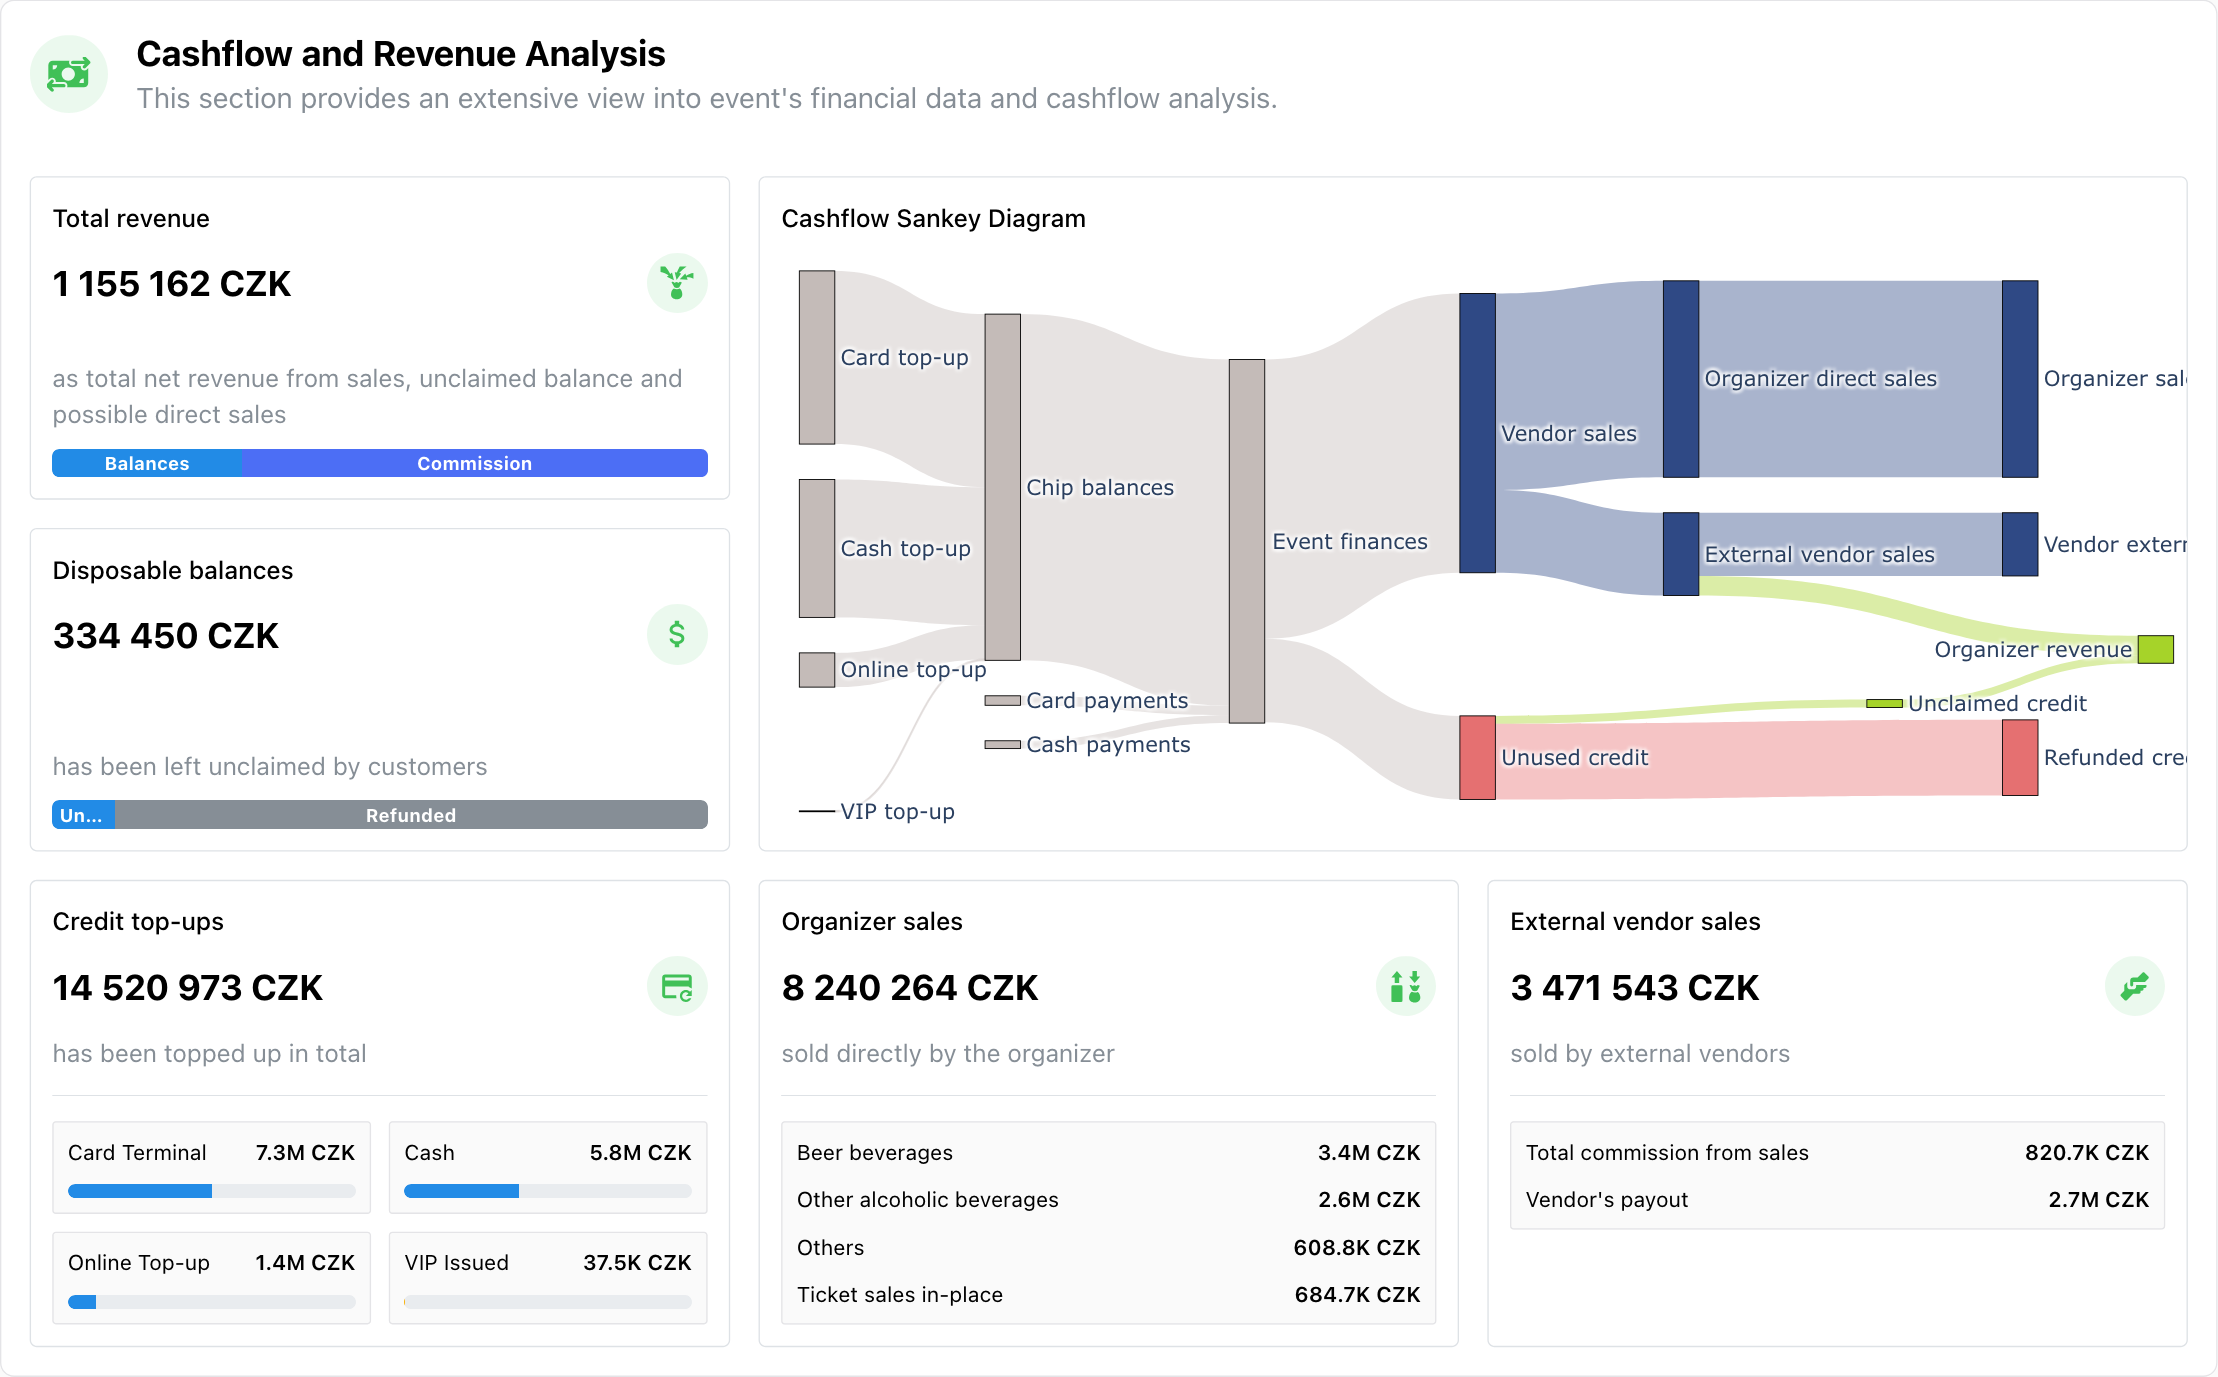
\includegraphics[width=\textwidth]{\ThesisFigures/ui/dashboard-cashflow-section}
			\caption{Cashflow and Revenue Analysis Section}
			\source
			\label{fig:dashboard-cashflow-analysis}
		\end{figure}

		The centerpiece Sankey diagram visualizes how money moves through the system—from initial top-ups through various payment channels to final settlements.
		This helps to track the conversion of chip credits into sales and monitor refund volumes.

		Below, sales data splits between organizer (\bfmtczk{8240264}) and vendor (\bfmtczk{3471543}) categories, with detailed breakdowns for beverages, food, and other revenue streams.
	\end{subsection}

	\begin{subsection}{Performance Analysis Section}
		\label{subsec:implementation-results-structure-performance}

		The performance section helps to understand operational dynamics throughout the festival.
		Key metrics prominently display the festival's scale: \bfmtnum{10009}~active customers, \bfmtnum{141378}~processed transactions, and a peak volume of~\bfmtnum{8986}~transactions per hour.

		\begin{figure}[H]
			\centering
			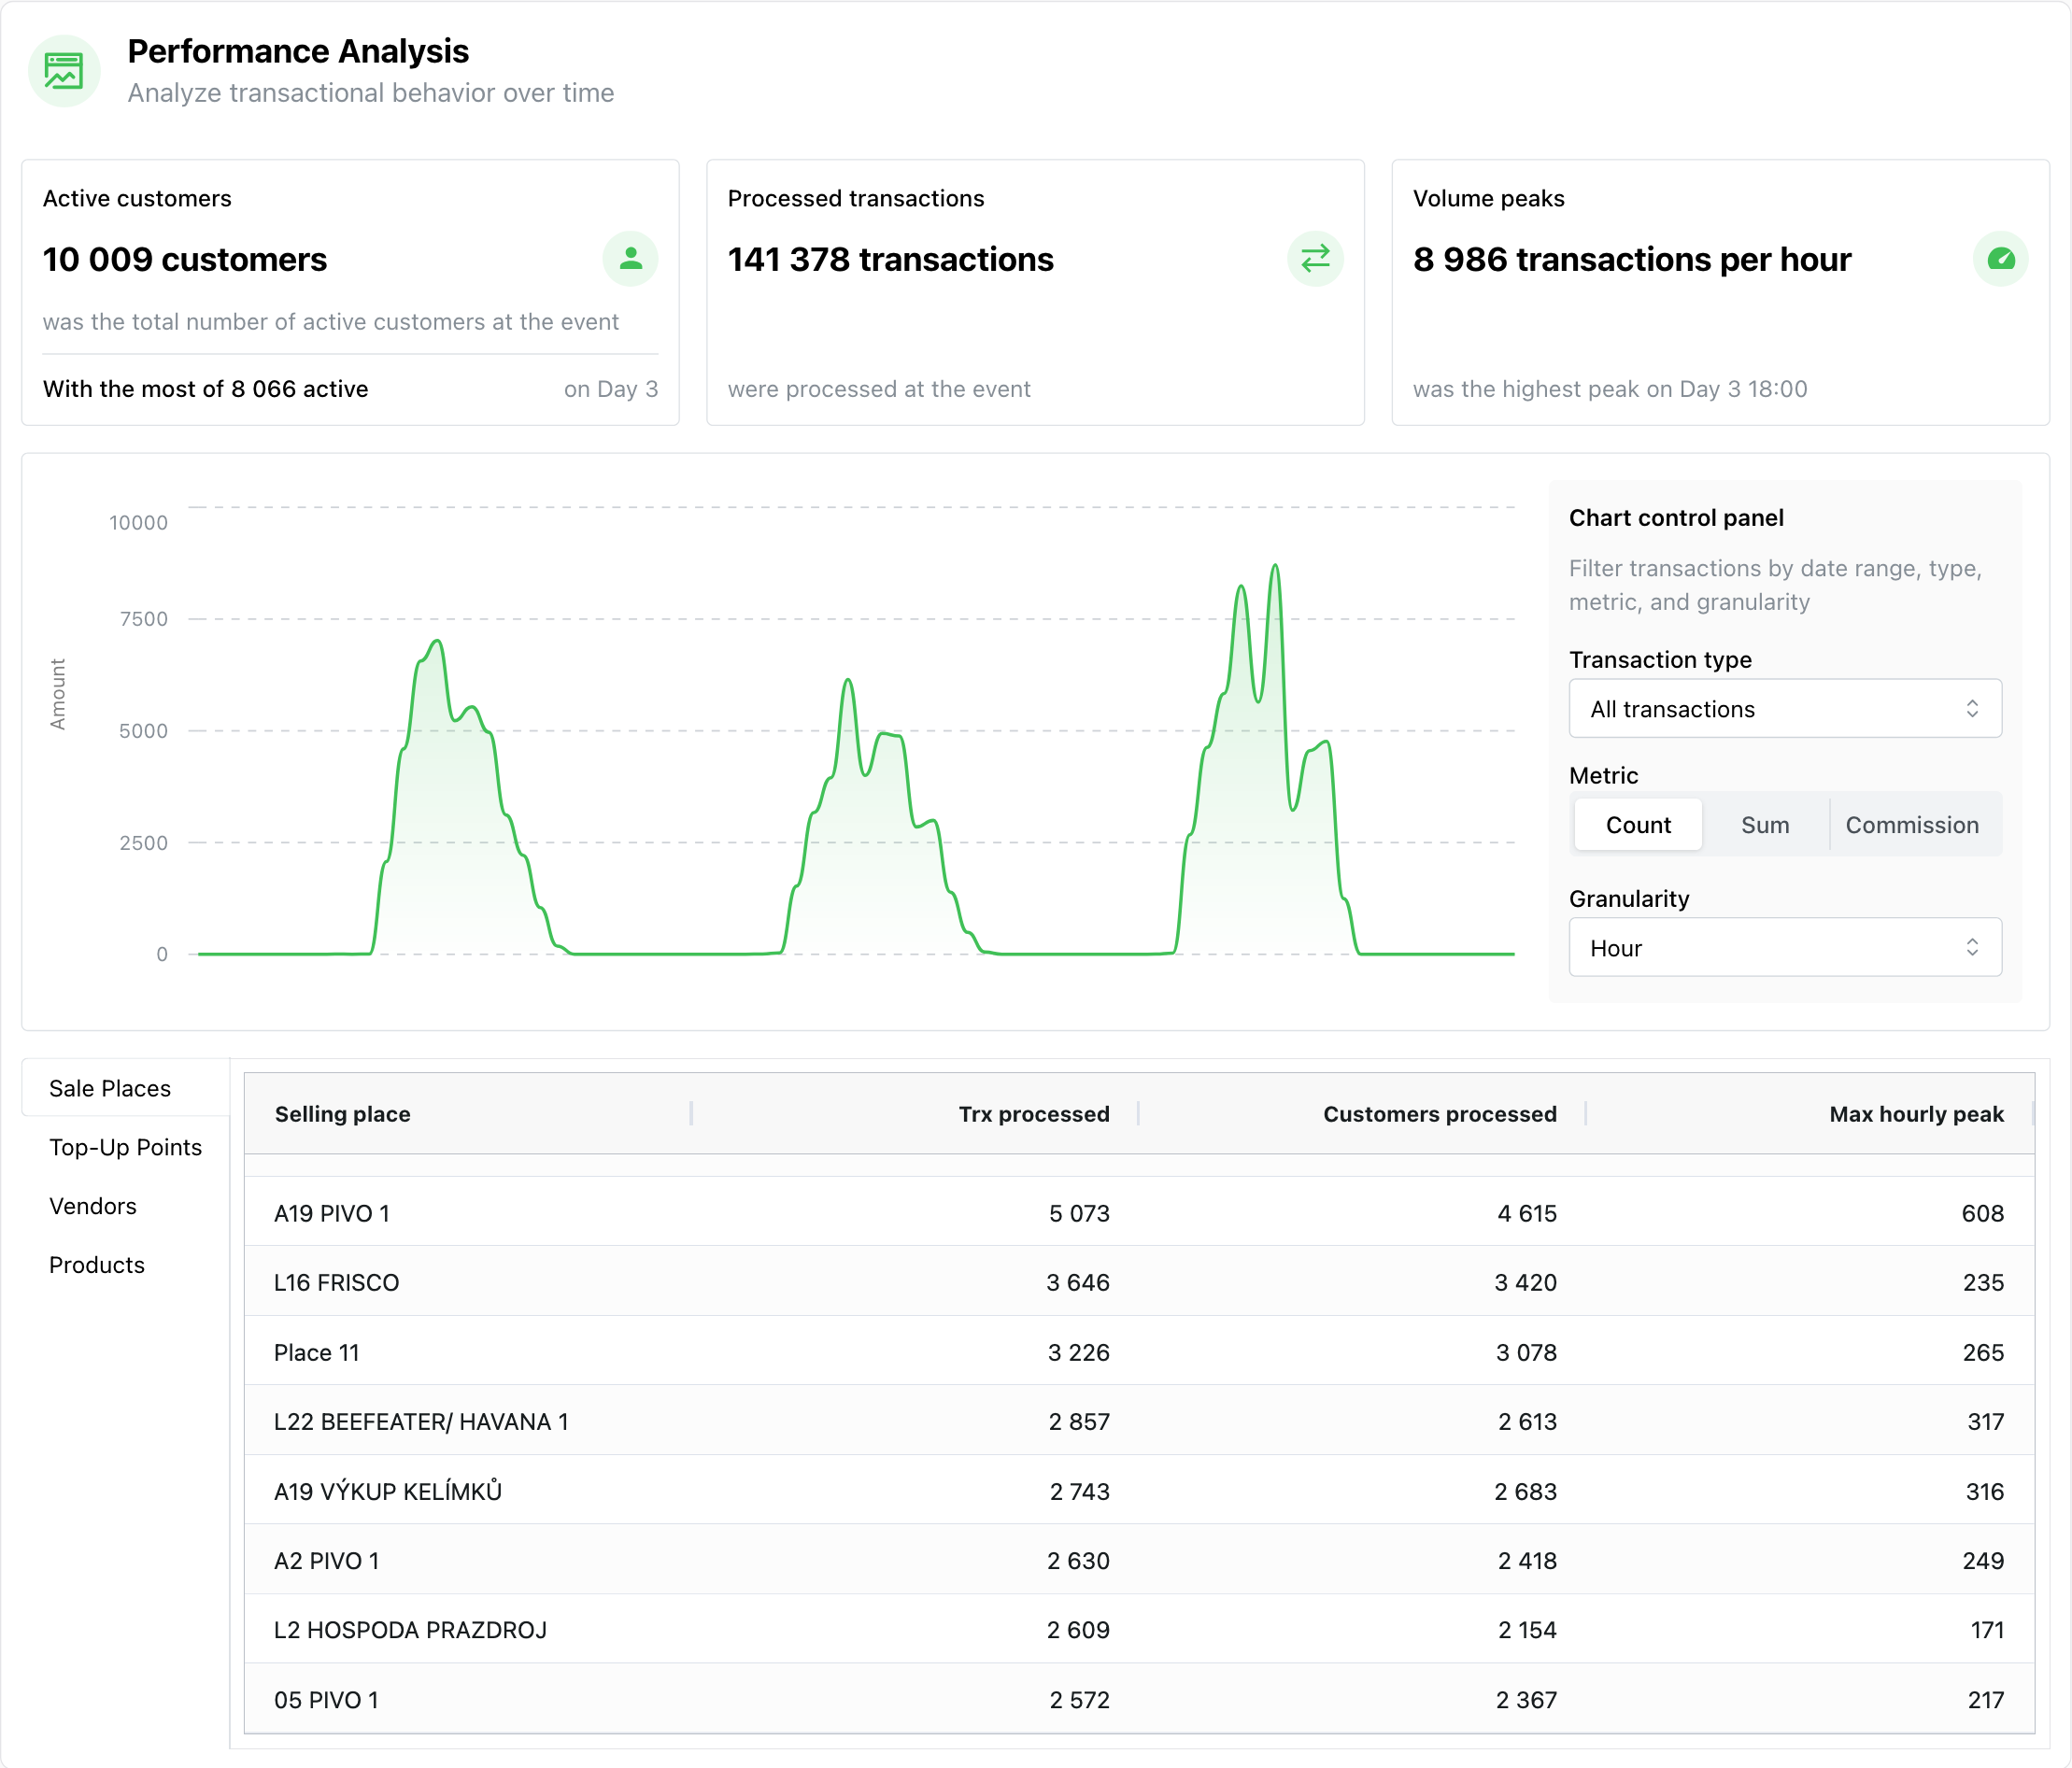
\includegraphics[width=\textwidth]{\ThesisFigures/ui/dashboard-performance-section}
			\caption{Performance Analysis Section}
			\source
			\label{fig:dashboard-performance-analysis}
		\end{figure}

		The main graph shows transaction volumes across all three days, with the highest peak visible on Day~3 at~18:00.

		The control panel can be used to filter by transaction types and adjust time granularity for detailed analysis.

		A table below highlights the busiest operational points, showing how many transactions and customers each location handled, as well as for individual vendors or products.
	\end{subsection}

	\begin{subsection}{Beverage Consumption Analysis Section}
		\label{subsec:implementation-results-structure-beverage}

		The beverage section tracks consumption patterns and returnable cup management.
		At a glance, a total consumption (\bfmtnum{29343}~liters), returnable cups issued (\bfmtnum{22045}), and the return rate of~\bfmtnump[2]{78.4}\% can immediately be seen.

		\begin{figure}[H]
			\centering
			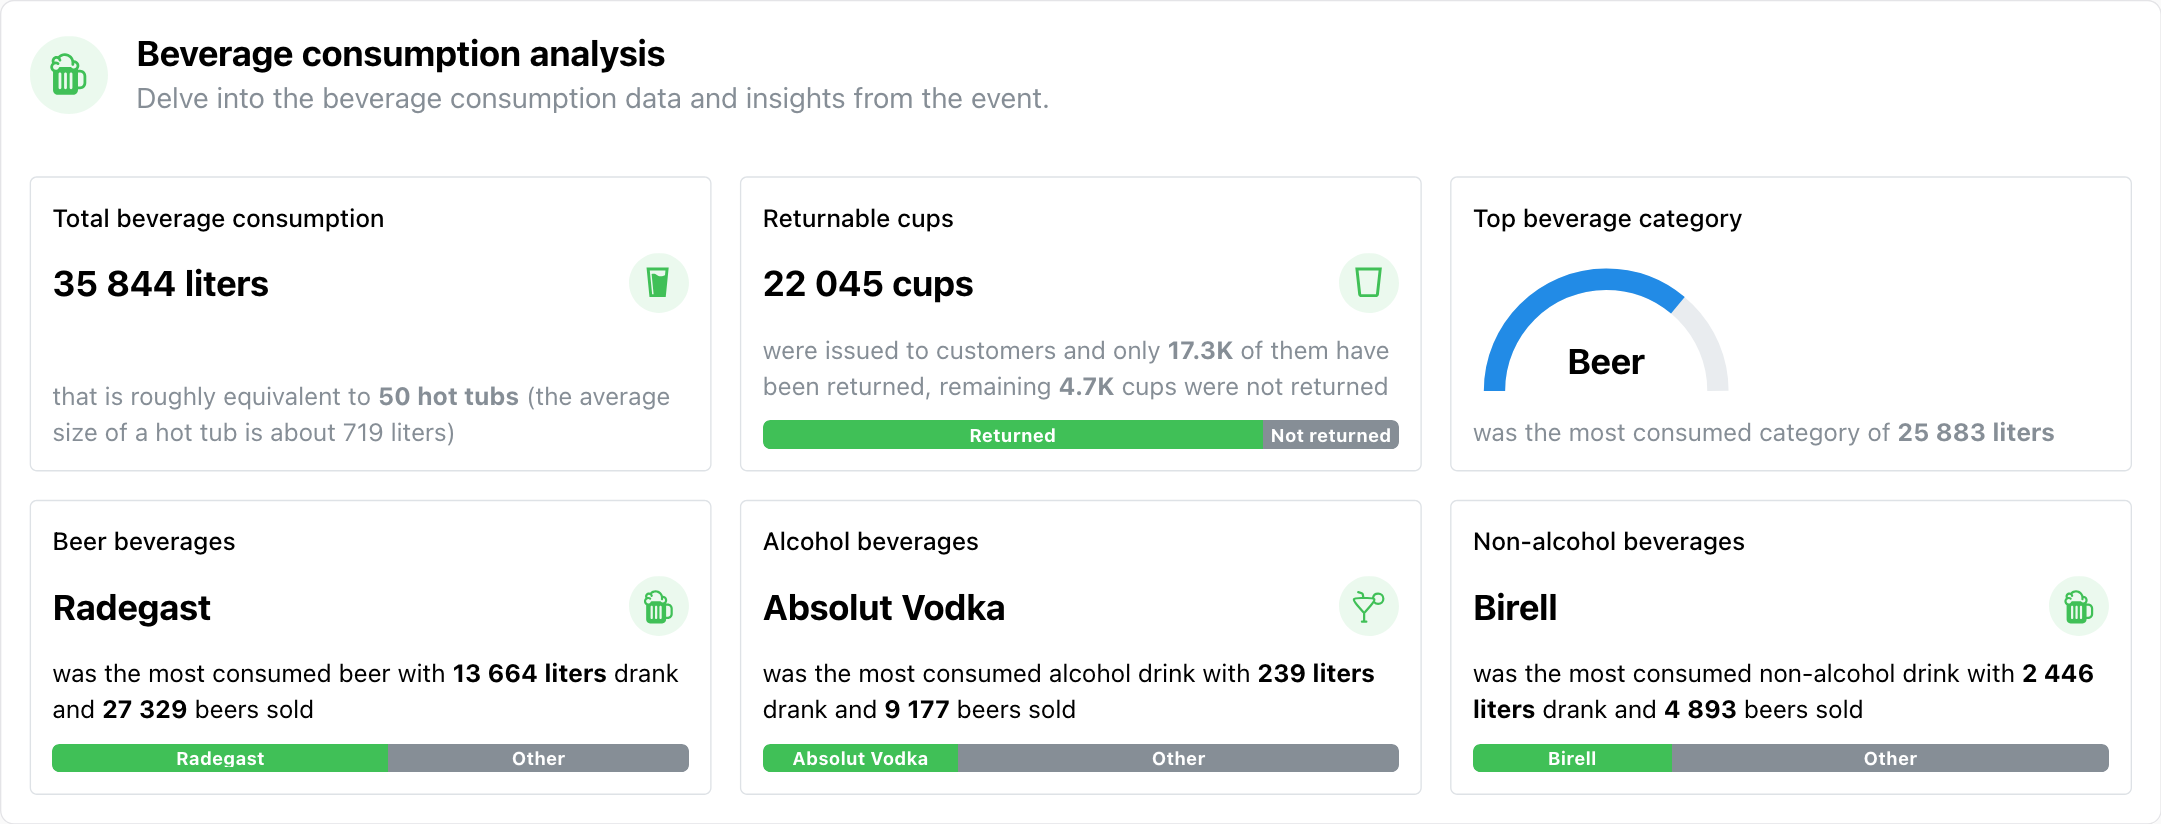
\includegraphics[width=\textwidth]{\ThesisFigures/ui/dashboard-beverage-section}
			\caption{Beverage Consumption Analysis Section}
			\source
			\label{fig:dashboard-beverage-analysis}
		\end{figure}

		Breaking down by category, \textbf{Radegast} led beer sales with \bfmtnum{10525}~liters and \bfmtnum{27752}~units sold.
		\textbf{Birell} dominated non-alcoholic beverages with \bfmtnum{21846}~liters, while \textbf{Beefeater} led spirits with \bfmtnum{966}~liters consumed.
	\end{subsection}

	\begin{subsection}{Customer Analysis Section}
		\label{subsec:implementation-results-structure-customer}

		While currently still in development, the customer analysis section aims to provide insights into attendee behavior patterns.
		The planned implementation focuses on four key areas of visitor analysis.

		\begin{figure}[H]
			\centering
			
\includegraphics[width=\textwidth]{\ThesisFigures/ui/dashboard-customer-section}
			\caption{Customer Analysis Section (Implementation in Progress)}
			\source
			\label{fig:dashboard-customer-analysis}
		\end{figure}

		The attendance timeline will show how \bfmtnum{10009}~unique visitors were distributed across the festival, with Day~3 seeing peak attendance of~\bfmtnum{8066}~visitors.
		Customer segmentation will break down the \bfmtnump[2]{89.66}\%~online ticket purchasers and track platform preferences, including the \bfmtnump[2]{40.69}\%~mobile app usage rate.
		Payment analysis will visualize card scheme preferences (VISA~\bfmtnump[2]{62.4}\%, Mastercard~\bfmtnump[2]{37.6}\%) and top-up patterns.

		This section represents a key area for future development, particularly for exploring customer behavior patterns.
		Unfortunately, due to the time constraints, it was not possible to finish the implementation of this section during the thesis project.
		However, the key findings from the analysis were already prepared and ready to be implemented.
	\end{subsection}
\end{section}


%%% Section: Missing Features and Future Development
%%% --------------------------------------------------------------
\begin{section}{Missing Features and Future Development}
	\label{sec:future-development}

	While the current implementation successfully demonstrates our analysis results, there are several directions for future development and improvement.

	\begin{subsection}{Technical Improvements}
		\label{subsec:future-technical}

		From a technical perspective, several key improvements would be needed for production deployment:

		\textbf{Infrastructure and Deployment}: The current implementation is limited to local setup with a local database.
		Significant architectural changes would be needed to enable external access and proper production deployment with a more robust database solution and data layer separation.

		\textbf{Performance Optimization}: SQL queries would require optimization for larger datasets.
		Implementation of materialized views\footnote{
			Materialized views are essentially database tables that store the results of a query and can be used to improve query performance\cite{tpgdg_current_rules_materializedviews}.
		} and better query planning would improve response times with production-scale data.

		\textbf{Caching Solution}: A production-grade caching system using Redis would replace the current development-focused implementation.
		This would improve dashboard responsiveness and enable handling multiple concurrent users.

		\textbf{Data Formatting}: Enhanced date formatting and chart configurations would improve data presentation.
		The current implementation uses basic formatting which would need refinement for production use.
	\end{subsection}

	\begin{subsection}{Analytical Enhancements}
		\label{subsec:future-analytical}

		From an analytical perspective, several key features would enhance the dashboard's utility:

		\textbf{Customer Analysis}: Complete implementation of the customer analysis section would provide valuable insights into attendee behavior.
		This would enable better understanding of customer segments and their preferences.

		\textbf{Performance Metrics}: Expansion of the performance section with detailed time processing metrics would provide better operational insights.
		This would help identify bottlenecks and optimization opportunities.

		\textbf{Timeline Navigation}: A dynamic timeline player would allow users to observe festival data evolution over time.
		This would enable to replay the festival's progression and identify critical moments or patterns.

		\textbf{Interactive Elements}: Additional interactive features would allow users to switch between different metrics and apply more granular filters.
		This flexibility would help to discover deeper insights and test different hypotheses about festival operations.
	\end{subsection}
\end{section}



	% ✅ chapter - conclusion
	%%% Conclusion
%%%%%%% Wording: ⏳
%%%%%%% Styling: ⏳
%%%%%%% References: ⏳
%%%%% Grammar: ⏳
%%% --------------------------------------------------------------
\chapter{Conclusion}
\label{ch:conclusion}


\begin{section}{Summary of Work}
	\label{sec:conclusion-summary}

	This thesis has been built upon two main pillars: \textbf{the analysis of the data collected by NFCtron's system} and \textbf{the development of an interactive dashboard} to visualize the findings.

	The analysis process started with the definition of the main research questions in cooperation with~\theOrganizer, resulting in a total of~\textbf{29 questions} to be answered.
	These questions were from a wide range of topics covering overall cashflow and revenue sources, system's performance, beverage consumption and customer behavior.
	A complete list of the research questions, together with the objectives of the analysis, are covered in the~\fullref{ch:introduction}~chapter.

	Before conducting the analysis, exploration of the data, followed by the identification of the main data quality issues and the data cleaning process, was necessary.
	This process covered also the local environment setup, the data import process, and the data model of the system, all thoroughly described in~\autoref{ch:data-methodology}.
	Followed by a simple data anonymization process, the data was ready for the analysis.

	The main part of the thesis, the data analysis itself, resulted in the most voluminous part of the thesis – that being~\autoref{ch:data-analysis-and-results}.
	It was divided into the four research areas: \fullref{sec:analysis-cashflow-and-revenue-sources}, \fullref{sec:analysis-performance-indicators}, \fullref{sec:analysis-beverage-consumption}, and~\fullref{sec:analysis-customers}.
	Each of these sections contained a detailed analysis of the data, answering the research questions in detail, presenting the findings in rich charts, diagrams and tables, providing the required insights.

	The final part of the thesis, development of the interactive dashboard, was based on the findings of the analysis.
	This process took significant time and effort, but resulted in an interactive dashboard that visualizes the most important findings of the analysis.
	Unfortunately, due to the time constraints, the dashboard was not fully completed, and some of the planned features were not implemented.
	The overall process of the implementation, ranging from the initial approach, through core architecture description, technical challenges faced and their solutions, to the final implementation results and presentation of the dashboard, is
	described in~\autoref{ch:dashboard-implementation}.

	The thesis now concludes with the reflections on the project, the professional impact and outcomes, and the future impact of the thesis on the NFCtron Hub system, as well as the final thoughts on the project.
\end{section}

\begin{section}{Reflections}
	\label{sec:conclusion-reflections}

	Working directly with festival data revealed both challenges and opportunities that may impact future development in the NFCtron system.

	From a data perspective, the analysis revealed several opportunities for improving data collection.
	The need to manually add beverage volume information highlighted a gap in the current system's data model, which can unlock great insights with minimal effort.
	Similarly, the value of combining transaction data with event scheduling information demonstrated the importance of comprehensive data integration for meaningful insights.

	The necessity of data anonymization for privacy reasons highlighted the importance of data protection and possible future challenges in this area.
	However, a simple data anonymization process was sufficient for the current analysis, and the data was successfully anonymized without losing its analytical value, providing a lesson for future data handling.

	From the analytical side, the analysis process revealed the importance of defining clear research questions and objectives before starting the analysis.
	Initially, without having clear research questions, the analysis process was challenging, ineffective and unstructured.
	However, this unstructured exploration phase was necessary to understand the data and to prepare multiple processes for the subsequent data inspection.
	It also taught me various SQL techniques and optimization methods, from which I benefited in the later stages of the analysis and surely will benefit in the future.

	After defining specific research questions, the analysis process became more focused, efficient and productive, leading to straightforward insights and findings.
	The presentation of the results was crucial for this analysis, but initially the data presentation was not optimal as preparing the data for the visualization is a meticulous process.
	If not done correctly, the results may be misleading or incorrect.
	However, with the right tools, techniques and adequate presentations, the results can be easily understood and interpreted.
	Thanks to the necessity to present data in a clear and understandable way, various better visualization charts were learned and used in the analysis.
	This included charts such as the waterfall chart, packed bubble chart or a simple pie chart alternative – the waffle chart.

	Finally, the development of the interactive dashboard was a challenging but rewarding process, and the technical challenges faced provided valuable lessons.
	While the initial impulse was often to implement complex~\enquote{proper}~solutions, simpler approaches frequently proved to be more effective and efficient.
	This was particularly obvious in the caching system evolution, where a straightforward file-based solution ultimately outperformed more sophisticated alternatives for development purposes.

	Many situations required a balance between the complexity of the solution and the time available for implementation.
	As a result, the dashboard was not fully completed, and some of the planned features were not implemented, which leaves room for future development and improvements.

	Overall, the thesis provided required insights into the data, the analysis process, and the development of interactive dashboards.
	It showed the importance of clear research questions, data quality and processing and an understandable data presentation for effective analysis results.
\end{section}

\begin{section}{Professional Impact and Outcomes}
	\label{sec:future-impact}

	The main personal motivation for this thesis was to learn more about the data and demonstrate the findings in an interactive way, leading to more insights and knowledge for future updates of the NFCtron Hub dashboard.

	The research and analysis process has already given new understanding and knowledge about the data, the SQL techniques and optimization methods.
	Thanks to this, I was already able to manage and deliver, together with my team, two significant updates to NFCtron Hub's analytical capabilities in late 2024.

	These updates resulted in a new time-based charts for ticket sales breakdowns and a comprehensive timeline view of festival activities including its sales, refunds, customer arrivals, and customer ratings.
	A simple preview of this new timeline component can be seen in~\autoref{fig:hub-chart-update} below.

	\begin{figure}[H]
		\centering
		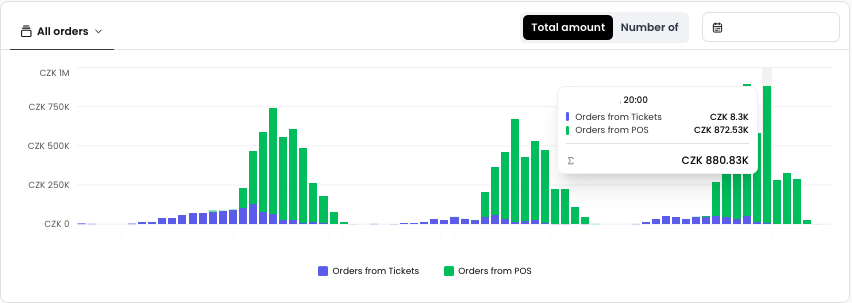
\includegraphics[width=\textwidth]{\ThesisFigures/ui/hub-chart-update}
		\caption{New Timeline Analysis in NFCtron Hub (December 2024 Update)}
		\label{fig:hub-chart-update}
		\source
	\end{figure}

	Also, thanks to the analytical findings and problems encountered during the analysis, I was able to provide valuable feedback to the development team.
	This will lead to improvements in the data collection process and the data model of the system, which will make future analysis easier and more efficient.

	Finally, the knowledge acquired by this thesis still shapes our product development and enables us to provide more advanced analytical capabilities to our clients – festival organizers.
	Future development will build upon these foundations, further expanding the analytical capabilities of NFCtron's system.
\end{section}
%%% ✅ bibliography
	\begin{flushleft}
		\bibliography{/Users/filipditrich/University/master_thesis/thesis/main,/Users/filipditrich/University/master_thesis/thesis/auto}
	\end{flushleft}
%%% ✅ list of figures
	\listoffigures
	\textit{Note: Unless stated otherwise, all figures are the author's rendition.}
%%% ✅ list of tables
	\listoftables
	\textit{Note: Unless stated otherwise, all tables are the author's rendition.}
%%% ✅ list of charts
	\listofcharts
	\textit{Note: Unless stated otherwise, all charts are the author's rendition.}
%%% ✅ list of source codes
	\listoflistings
%%% ⏳ appendix | TODO: Create ZIP and attach it after final revisions
	%%% List of Appendices
%%%%%%% Wording: ✅
%%%%%%% Styling: ✅
%%%%%%% References: ✅
%%%%% Grammar: ✅
%%% --------------------------------------------------------------
\appendix
\addtocontents{toc}{\protect\setlength{\cftsecnumwidth}{22mm}}
\chapter*{List of Appendices}
\addcontentsline{toc}{chapter}{List of Appendices}
\renewcommand{\thesection}{Appendix \Alph{section}}

%%% Appendix A: Source code of the application
%%%%% File preparation: ⏳
%%%%% Instructions: ✅
%%% --------------------------------------------------------------
\begin{section}{Source code of the application}
	\label{appendix:source-code}
	The source code for the dashboard application is available on the attached CD in the~\texttt{dashboard\_app.zip} file.

	The application is built using Python 3.9\footnote{\url{https://www.python.org/downloads/release/python-390/}}, and its requirements are listed in the~\texttt{requirements.txt} file.

	The application is structured as follows:
	\begin{itemize}
		\item \texttt{app.py}: the main Dash application implementation
		\item \texttt{queries\/}: directory with SQL queries
		\item \texttt{sections\/}: directory with implementation of dashboard sections
		\item \texttt{assets\/}: directory with CSS stylesheets
		\item \texttt{\_dash\_utils.py}: utility functions for Dash
		\item \texttt{\_db\_utils.py}: common database utility functions with query manager implementation
		\item \texttt{\_query\_manager.py}: registered SQL queries
		\item \texttt{\_format\_utils.py}: utility functions for data formatting
		\item \texttt{\_chart\_utils.py}: utility functions for chart generation, SankeyDiagram implementation
	\end{itemize}

\end{section}
\newpage
%%% ⏳ extended summary | TODO: Extended Summary document creation
	\addtocontents{toc}{\protect\contentsline{chapter}{Extended Summary}{}{}}
\end{document}
